\documentclass[aspectratio=169]{beamer}
% ============================================================================
% HEC Montréal MBA -- ECON50803: Macroeconomic Environment
% Shared Beamer Preamble
% ============================================================================

% --- Theme and base settings ------------------------------------------------
\usetheme{default}
\setbeamersize{text margin left=1.2cm, text margin right=1.2cm}

% --- Fonts ------------------------------------------------------------------
% Sans-serif throughout for a business look (comment out FiraSans if unavailable)
\usepackage[sfdefault,light]{FiraSans}
\usepackage{FiraMono}
\usepackage[T1]{fontenc}
\usepackage[utf8]{inputenc}
\setbeamerfont{title}{series=\bfseries, size=\Large}
\setbeamerfont{frametitle}{series=\bfseries, size=\large}
\setbeamerfont{framesubtitle}{series=\mdseries, size=\normalsize}

% --- Colors -----------------------------------------------------------------
\definecolor{HECnavy}{HTML}{002855}
\definecolor{HECgreen}{HTML}{26d07c}
\definecolor{HECcoral}{HTML}{ff585d}
\definecolor{HECtext}{HTML}{2D3748}
\definecolor{HECgray}{HTML}{94A3B8}
\definecolor{HEClightgray}{HTML}{F1F5F9}
\definecolor{HEClightblue}{HTML}{E8EDF3}

% Beamer color assignments
\setbeamercolor{normal text}{fg=HECtext}
\setbeamercolor{title}{fg=HECnavy}
\setbeamercolor{frametitle}{fg=HECnavy}
\setbeamercolor{structure}{fg=HECnavy}
\setbeamercolor{background canvas}{bg=white}
\setbeamercolor{alerted text}{fg=HECcoral}
\setbeamercolor{example text}{fg=HECgreen}
\hypersetup{colorlinks, linkcolor=HECnavy, urlcolor=HECnavy, citecolor=HECtext}

% --- Navigation and chrome --------------------------------------------------
\setbeamertemplate{navigation symbols}{}

% Frame title: bold text with a thin accent line
\setbeamertemplate{frametitle}{%
   \vspace{0.25cm}%
   {\usebeamerfont{frametitle}\usebeamercolor[fg]{frametitle}\insertframetitle}%
   \ifx\insertframesubtitle\empty\else%
      \\[2pt]{\usebeamerfont{framesubtitle}\textcolor{HECgray}{\insertframesubtitle}}%
   \fi%
   \\[-4pt]\textcolor{HECgreen}{\rule{2.5cm}{1.5pt}}%
   \\[-2pt]%
}

% Footer: course name left, slide number right, thin rule above
\setbeamertemplate{footline}{%
   \vspace{-0.1cm}%
   \hbox to \paperwidth{%
      \hspace{1.2cm}%
      \textcolor{HEClightgray}{\rule{0.84\paperwidth}{0.4pt}}%
      \hspace{1.2cm}%
   }%
   \vspace{0.05cm}%
   \hbox to \paperwidth{%
      \hspace{1.2cm}%
      {\scriptsize\textcolor{HECgray}{ECON 50803\enspace\textbar\enspace Environnement macroéconomique}}%
      \hfill%
      {\scriptsize\textcolor{HECgray}{\insertframenumber}}%
      \hspace{1.2cm}%
   }%
   \vspace{0.15cm}%
}

% --- Itemize/enumerate styling ----------------------------------------------
\setbeamertemplate{itemize item}{\textcolor{HECnavy}{$\bullet$}}
\setbeamertemplate{itemize subitem}{\textcolor{HECgray}{$\bullet$}}
\setbeamertemplate{itemize subsubitem}{\textcolor{HECgray}{\scalebox{0.6}{$\blacktriangleright$}}}
\setbeamertemplate{enumerate item}{\textcolor{HECnavy}{\bfseries\insertenumlabel.}}
\setbeamertemplate{enumerate subitem}{\textcolor{HECgray}{\insertsubenumlabel.}}

% --- Packages ---------------------------------------------------------------
\usepackage{
   tikz, caption, subcaption, ragged2e, amsmath, bm,
   makecell, threeparttable, booktabs, mathtools,
   multirow, calc, hyperref, tabularx, colortbl,
   transparent, tcolorbox, xcolor, graphicx
}
\usepackage[round]{natbib}
\usetikzlibrary{decorations.pathreplacing, decorations.markings, calc, arrows.meta, positioning}
\usepackage[absolute,overlay]{textpos}
\captionsetup[figure]{labelformat=empty, font=small, textfont=it}
\captionsetup[table]{labelformat=empty, font=small}
\setlength{\belowcaptionskip}{0cm}
\apptocmd{\frame}{}{\justifying}

% --- Paths ------------------------------------------------------------------
\graphicspath{{../Figures/}}
\newcommand*\includetables[1]{\input{../Tables/#1.tex}}

% --- Mathematical commands --------------------------------------------------
\DeclareMathOperator*{\argmax}{arg\,max}
\newcommand{\partialof}[2]{\frac{\partial #1}{\partial #2}}
\newcommand{\totalof}[2]{\frac{\text{d}#1}{\text{d}#2}}
\newcommand{\pctchg}[1]{\%\Delta #1}
\newcommand{\smallquad}{\hspace{0.5em}}

% --- Resize equation command ------------------------------------------------
\newcommand{\resizeeq}[2]{\resizebox{#2\hsize}{!}{$#1$}}

% ============================================================================
% CUSTOM SLIDE TYPES
% ============================================================================

% --- Title slide (call with \titleframe) ------------------------------------
\newcommand{\titleframe}{%
   {\setbeamertemplate{footline}{}%
   \begin{frame}[plain]
      \begin{tikzpicture}[remember picture, overlay]
         % Navy accent bar on the left
         \fill[HECnavy] (current page.north west) rectangle
            ([xshift=0.6cm]current page.south west);
         % Green accent line
         \fill[HECgreen] ([xshift=0.6cm]current page.north west) rectangle
            ([xshift=0.65cm]current page.south west);
      \end{tikzpicture}
      \vspace{1cm}
      \hspace{0.6cm}%
      \begin{minipage}{0.85\textwidth}
         {\usebeamerfont{title}\usebeamercolor[fg]{title}\inserttitle}
         \\[12pt]
         \textcolor{HECgreen}{\rule{3cm}{2pt}}
         \\[12pt]
         {\large\textcolor{HECgray}{\insertauthor}}
         \\[6pt]
         {\normalsize\textcolor{HECgray}{\insertdate}}
      \end{minipage}
      \vfill
      \hspace{0.6cm}%
      {\footnotesize\textcolor{HECgray}{HEC Montréal \enspace\textbar\enspace MBA}}
      \vspace{0.5cm}
   \end{frame}}%
}

% --- Section divider slide --------------------------------------------------
\newcommand{\sectionframe}[1]{%
   {\setbeamertemplate{footline}{}%
   \begin{frame}[plain]
      \begin{tikzpicture}[remember picture, overlay]
         \fill[HECnavy] ([shift={(-1pt,1pt)}]current page.north west) rectangle
            ([shift={(1pt,-1pt)}]current page.south east);
         \node[anchor=center] at (current page.center) {%
            \begin{minipage}{0.8\paperwidth}
               \centering
               {\LARGE\bfseries\textcolor{white}{#1}}
               \\[12pt]
               \textcolor{HECgreen}{\rule{3cm}{2pt}}
            \end{minipage}
         };
      \end{tikzpicture}
   \end{frame}}%
}

% ============================================================================
% CUSTOM BOX ENVIRONMENTS
% ============================================================================

% Key Insight (green accent)
\newtcolorbox{keyinsight}[1][Point clé]{%
   colback=HECgreen!5,
   colframe=HECgreen,
   boxrule=0pt,
   leftrule=3pt,
   arc=8pt,
   title={\textcolor{HECgreen}{\bfseries #1}},
   coltitle=HECgreen,
   fonttitle=\bfseries,
   attach title to upper={\\[4pt]},
   left=10pt, right=10pt, top=6pt, bottom=6pt
}

% Business Implication (navy accent)
\newtcolorbox{bizimplication}[1][Implication d'affaires]{%
   colback=HECnavy!5,
   colframe=HECnavy,
   boxrule=0pt,
   leftrule=3pt,
   arc=8pt,
   title={\textcolor{HECnavy}{\bfseries #1}},
   coltitle=HECnavy,
   fonttitle=\bfseries,
   attach title to upper={\\[4pt]},
   left=10pt, right=10pt, top=6pt, bottom=6pt
}

% Warning / Important (coral accent)
\newtcolorbox{warning}[1][Important]{%
   colback=HECcoral!5,
   colframe=HECcoral,
   boxrule=0pt,
   leftrule=3pt,
   arc=8pt,
   title={\textcolor{HECcoral}{\bfseries #1}},
   coltitle=HECcoral,
   fonttitle=\bfseries,
   attach title to upper={\\[4pt]},
   left=10pt, right=10pt, top=6pt, bottom=6pt
}

% Definition (gray background)
\newtcolorbox{defbox}[1][Définition]{%
   colback=HEClightgray,
   colframe=HEClightgray,
   boxrule=0pt,
   leftrule=3pt,
   arc=8pt,
   left=10pt, right=10pt, top=6pt, bottom=6pt,
   title={\textcolor{HECnavy}{\bfseries #1}},
   coltitle=HECnavy,
   fonttitle=\bfseries,
   attach title to upper={\\[4pt]}
}

% In-Class Exercise (coral accent)
\newtcolorbox{exercise}[1][Exercice]{%
   colback=HECcoral!5,
   colframe=HECcoral,
   boxrule=0pt,
   leftrule=3pt,
   arc=8pt,
   title={\textcolor{HECcoral}{\bfseries #1}},
   coltitle=HECcoral,
   fonttitle=\bfseries,
   attach title to upper={\\[4pt]},
   left=10pt, right=10pt, top=6pt, bottom=6pt
}

% ============================================================================
% NEWSPAPER HEADLINES SLIDE TEMPLATE
% ============================================================================
% Usage: inside a frame, open a tikzpicture[remember picture, overlay], then:
%   \setcounter{newshl}{0}
%   \newsheadline{Newspaper Name}{``Headline text''}   % up to 6 entries
%   \headlinesoverlay{Large overlay text}               % optional 2nd slide
%
% Headlines are auto-positioned in a 2×3 staggered grid (left/right alternating).
%
% Logo support: place PNG files in Figures/logos/ (e.g., ft.png, economist.png).
% Use the optional argument to specify the logo file (without extension):
%   \newsheadline[ft]{Financial Times}{Headline text}   % logo + bold headline
%   \newsheadline{The Economist}{``Headline text''}      % text-only fallback

\newcounter{newshl}

\newcommand{\newsheadline}[3][]{%
   % #1 = optional logo file key (e.g., ft → logos/ft.png)
   % #2 = newspaper name (text fallback when no logo)
   % #3 = headline text
   \stepcounter{newshl}%
   \pgfmathsetmacro{\hlrow}{int((\thenewshl-1)/2)}%
   \pgfmathsetmacro{\hlcol}{int(mod(\thenewshl-1,2))}%
   \pgfmathsetmacro{\hlx}{0.8 + \hlcol * 7.8}%
   \pgfmathsetmacro{\hly}{-1.5 - \hlrow * 2.0}%
   \node[anchor=north west]
      at ([shift={(\hlx cm,\hly cm)}]current page.north west) {%
      \ifx\\#1\\%
         \begin{minipage}[t]{5.8cm}%
            \textbf{\textcolor{HECgray}{\footnotesize\MakeUppercase{#2}}}%
            \\[-1pt]%
            {\small\itshape #3}%
         \end{minipage}%
      \else%
         \begin{minipage}[c]{1.2cm}%
            \includegraphics[height=1.2cm]{logos/#1}%
         \end{minipage}%
         \hspace{6pt}%
         \begin{minipage}[c][1.2cm][c]{4.3cm}%
            \raggedright{\small\textcolor{HECtext!75}{#3}}%
         \end{minipage}%
      \fi%
   };%
}

\newcommand{\headlinesoverlay}[1]{%
   \only<2>{%
      \fill[white, opacity=0.85]
         (current page.south west) rectangle (current page.north east);%
      \node[anchor=center] at ([yshift=-0.5cm]current page.center) {%
         {\fontsize{36}{44}\selectfont\bfseries\textcolor{HECnavy}{#1}}%
      };%
   }%
}

% ============================================================================
% NAVIGATION BUTTONS (optional, for bottom-of-slide section nav)
% ============================================================================

\newlength{\buttonwidth}
\newlength{\currentxpos}
\setlength{\currentxpos}{1.2cm}
\newlength{\buttonsep}
\setlength{\buttonsep}{0.05cm}

\newcommand{\mybutton}[2]{%
   \settowidth{\buttonwidth}{#1}%
   \begin{textblock*}{\buttonwidth + 2ex}(\currentxpos, \paperheight - 2.5em)
      \hyperlink{#2}{\beamerbutton{#1}}
   \end{textblock*}%
   \addtolength{\currentxpos}{\buttonwidth + \buttonsep}%
}

% ============================================================================
% BACKUP SLIDES SUPPORT
% ============================================================================

\newcommand{\backupbegin}{%
   \newcounter{finalframe}%
   \setcounter{finalframe}{\value{framenumber}}%
}
\newcommand{\backupend}{%
   \setcounter{framenumber}{\value{finalframe}}%
}


\title{The macroeconomic landscape}
\author{Jean-F\'elix Brouillette}
\date{Session 1}

\begin{document}

% ============================================================================
\titleframe
% ============================================================================

% --- Slide 1: What is macroeconomics?
\begin{frame}{What is macroeconomics?}
   \textbf{Macroeconomics deals with\ldots}
   \vspace{0.15cm}
   \begin{itemize}
      \setlength\itemsep{0.2cm}
      \item Global economic phenomena: the \textbf{big picture}
      \item \textbf{Interconnections} between economic agents (e.g., consumers, firms, gov.)
      \item \textbf{Long-run} trends, \textbf{short-run} fluctuations, and economic \textbf{policy}
   \end{itemize}
   \vspace{0.4cm}
   \textbf{Macroeconomics is closely linked to many other fields:}
   \vspace{0.15cm}
   \begin{itemize}
      \setlength\itemsep{0.15cm}
      \item Politics and geopolitics
      \item Psychology and sociology
      \item Finance
      \item Environment, technology, etc.
   \end{itemize}
\end{frame}

% --- Slide 2: Macro vs. micro ---
\begin{frame}{Macroeconomics vs.\ microeconomics}
   \textbf{Microeconomics} provides great tools to study how individuals make decisions\ldots
   \\[6pt]
   \ldots but not how they \textbf{aggregate} to the economy as a whole
   \\[6pt]
   \ldots and this aggregation, in turn, matters \textbf{a lot} for individual decision-making!
   \vspace{0.5cm}

   \textbf{When individual rationality leads to collective madness\ldots}
   \vspace{0.2cm}
   \begin{itemize}
      \setlength\itemsep{0.2cm}
      \item \textbf{The paradox of thrift:} everyone saves more in a recession
      \item \textbf{Helicopter money:} too many dollars chasing too few goods
      \item \textbf{The fallacy of composition:} standing up at a hockey game
   \end{itemize}
\end{frame}

% --- Slide 3: Why should you care? (adapted from Vincent S1 slide 3) ---
\begin{frame}{Why should \textit{you} care about macroeconomics?}
   The success of any business decision rests partly on \textbf{macroeconomic conditions} \\
   \vspace{0.3cm}

   Macroeconomic events, forces, and trends\ldots
   \vspace{0.15cm}
   \begin{enumerate}
      \setlength\itemsep{0.2cm}
      \item \ldots disrupt \textbf{business strategies}
      \item \ldots influence \textbf{costs, wages, interest rates}, and \textbf{competition}
      \item \ldots are sources of \textbf{risk}, but also of \textbf{opportunity}
      \item \ldots shape \textbf{markets} on a global scale \\
   \end{enumerate}
   \vspace{0.3cm}

   \ldots and \textbf{macroeconomic jargon} will be at the heart of conversations you will have as future managers
\end{frame}

% --- Slides 4--5: Headlines collage + "Where are we now?" overlay ---
\begin{frame}{A complex and uncertain world}
   \begin{tikzpicture}[remember picture, overlay]
      \setcounter{newshl}{0}
      \newsheadline[economist]{The Economist}{``Who wrangled the best trade deal from Donald Trump?''}
      \newsheadline[bloomberg]{Bloomberg}{``Kevin Warsh’s Fed Job Already Looks Impossible''}
      \newsheadline[ft]{Financial Times}{``Gold rips past \$5,000 on fears of global turmoil''}
      \newsheadline[lapresse]{La Presse}{``Les exportations du Québec en forte baisse''}
      \newsheadline[globeandmail]{The Globe and Mail}{``Mark Carney’s speech got the world’s attention---but was it the right message?''}
      \newsheadline[wsj]{The Wall Street Journal}{``The Big Money in Today’s Economy Is Going to Capital, Not Labor''}
      \headlinesoverlay{Where are we now?}
   \end{tikzpicture}
\end{frame}

% --- Narrative arc: 6 slides after "Where are we now?" ---

% Slide N1: After a very unusual recession...
\begin{frame}{After a very unusual recession\ldots}
   \begin{figure}
      \centering
      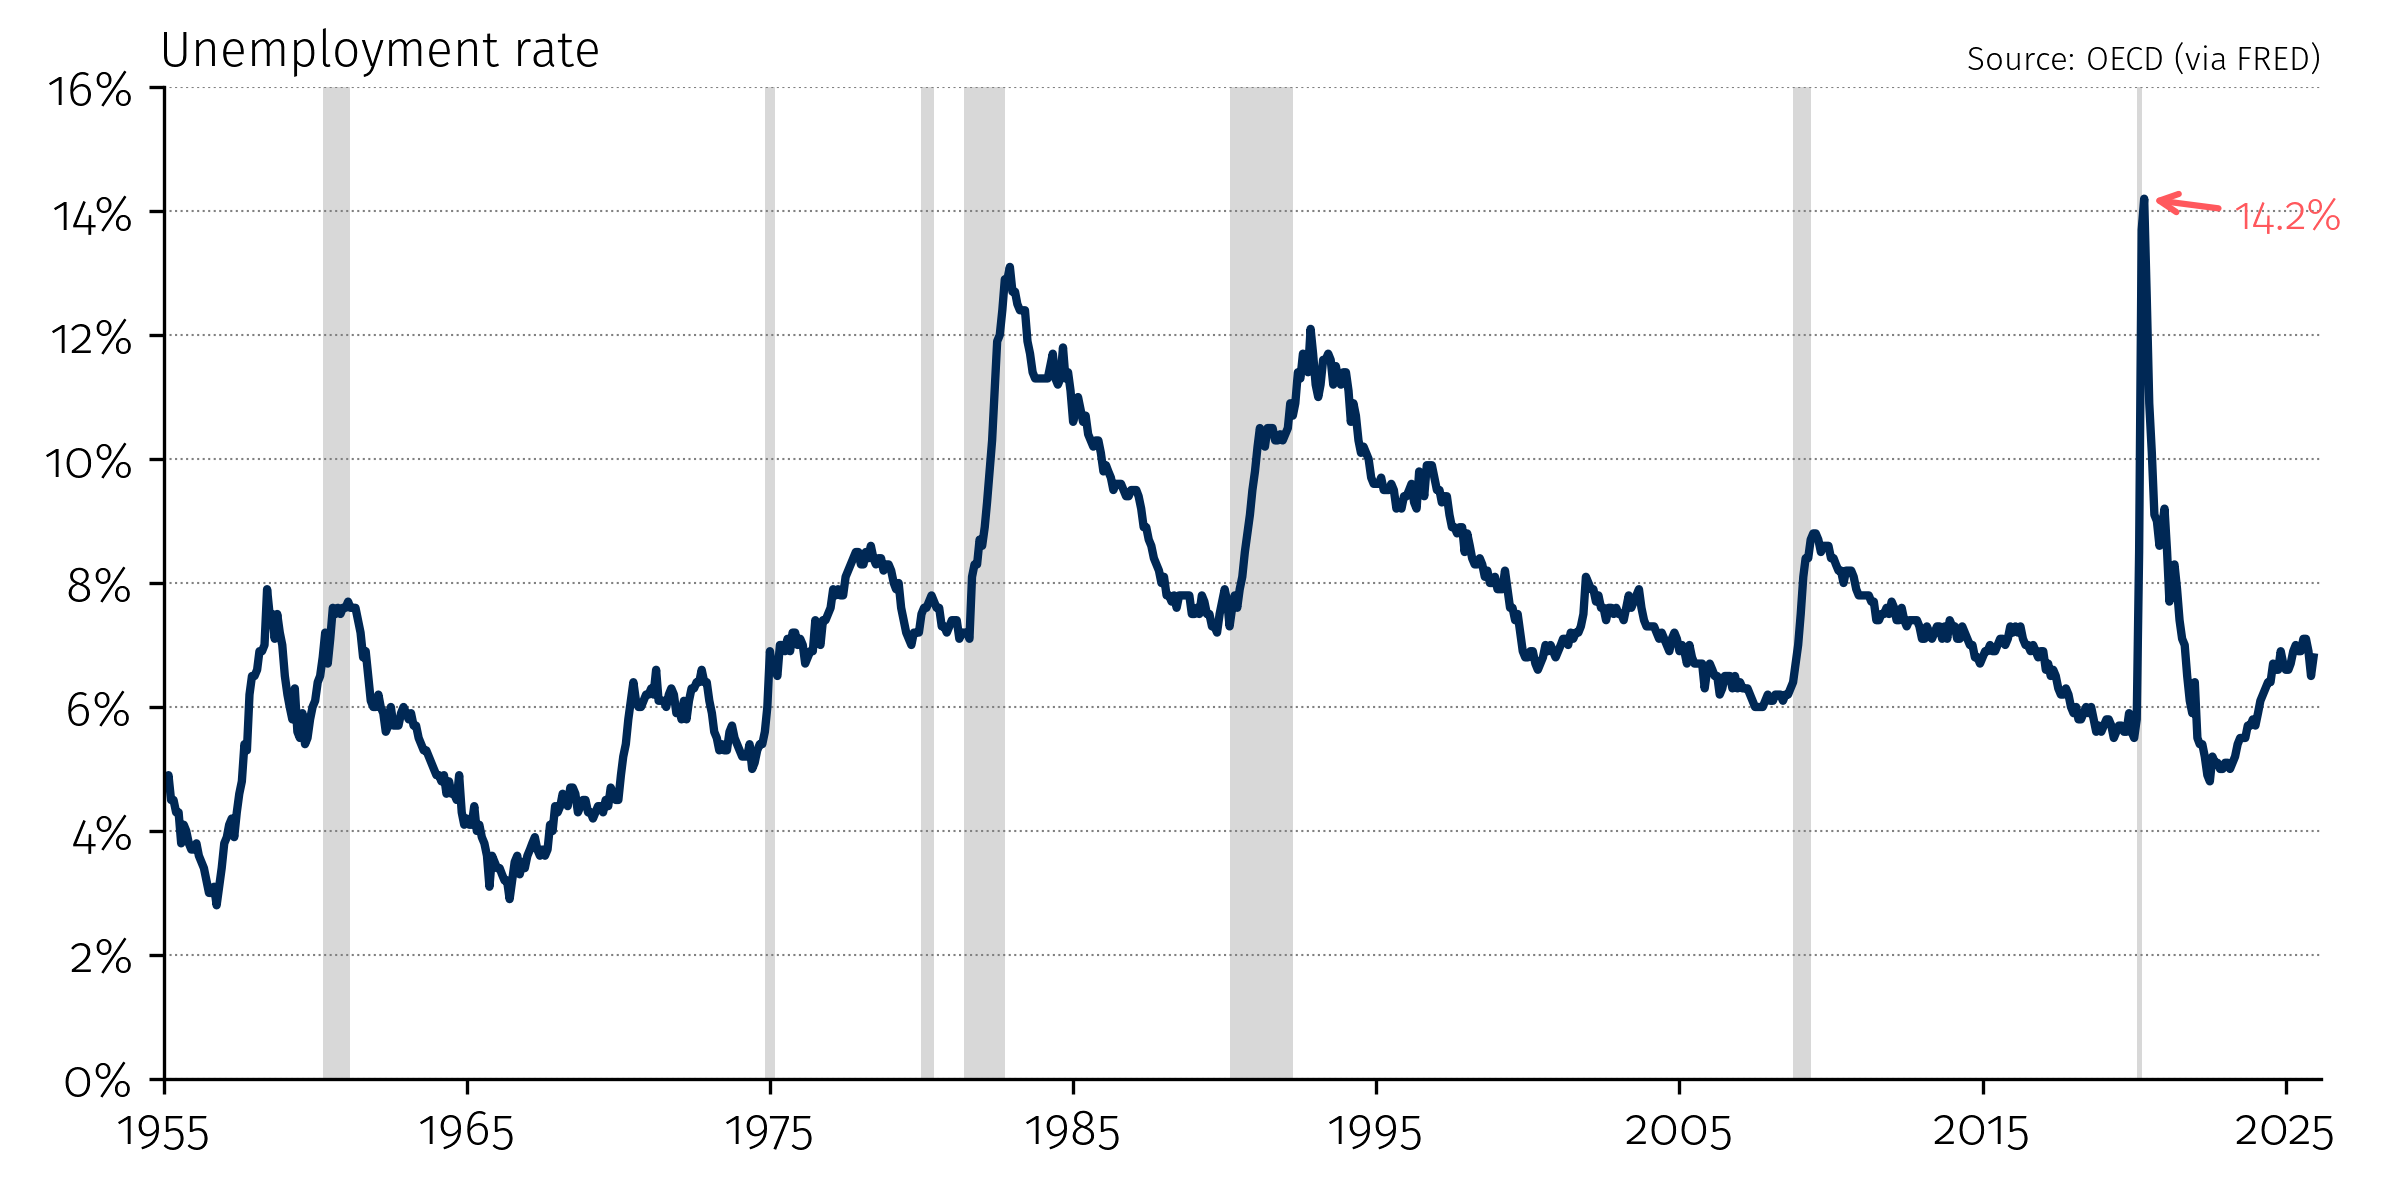
\includegraphics[width=0.9\textwidth]{can_unemployment.png}
   \end{figure}
\end{frame}

% Slide N2: An old enemy back from the dead...
\begin{frame}{An old enemy back from the dead\ldots}
   \begin{figure}
      \centering
      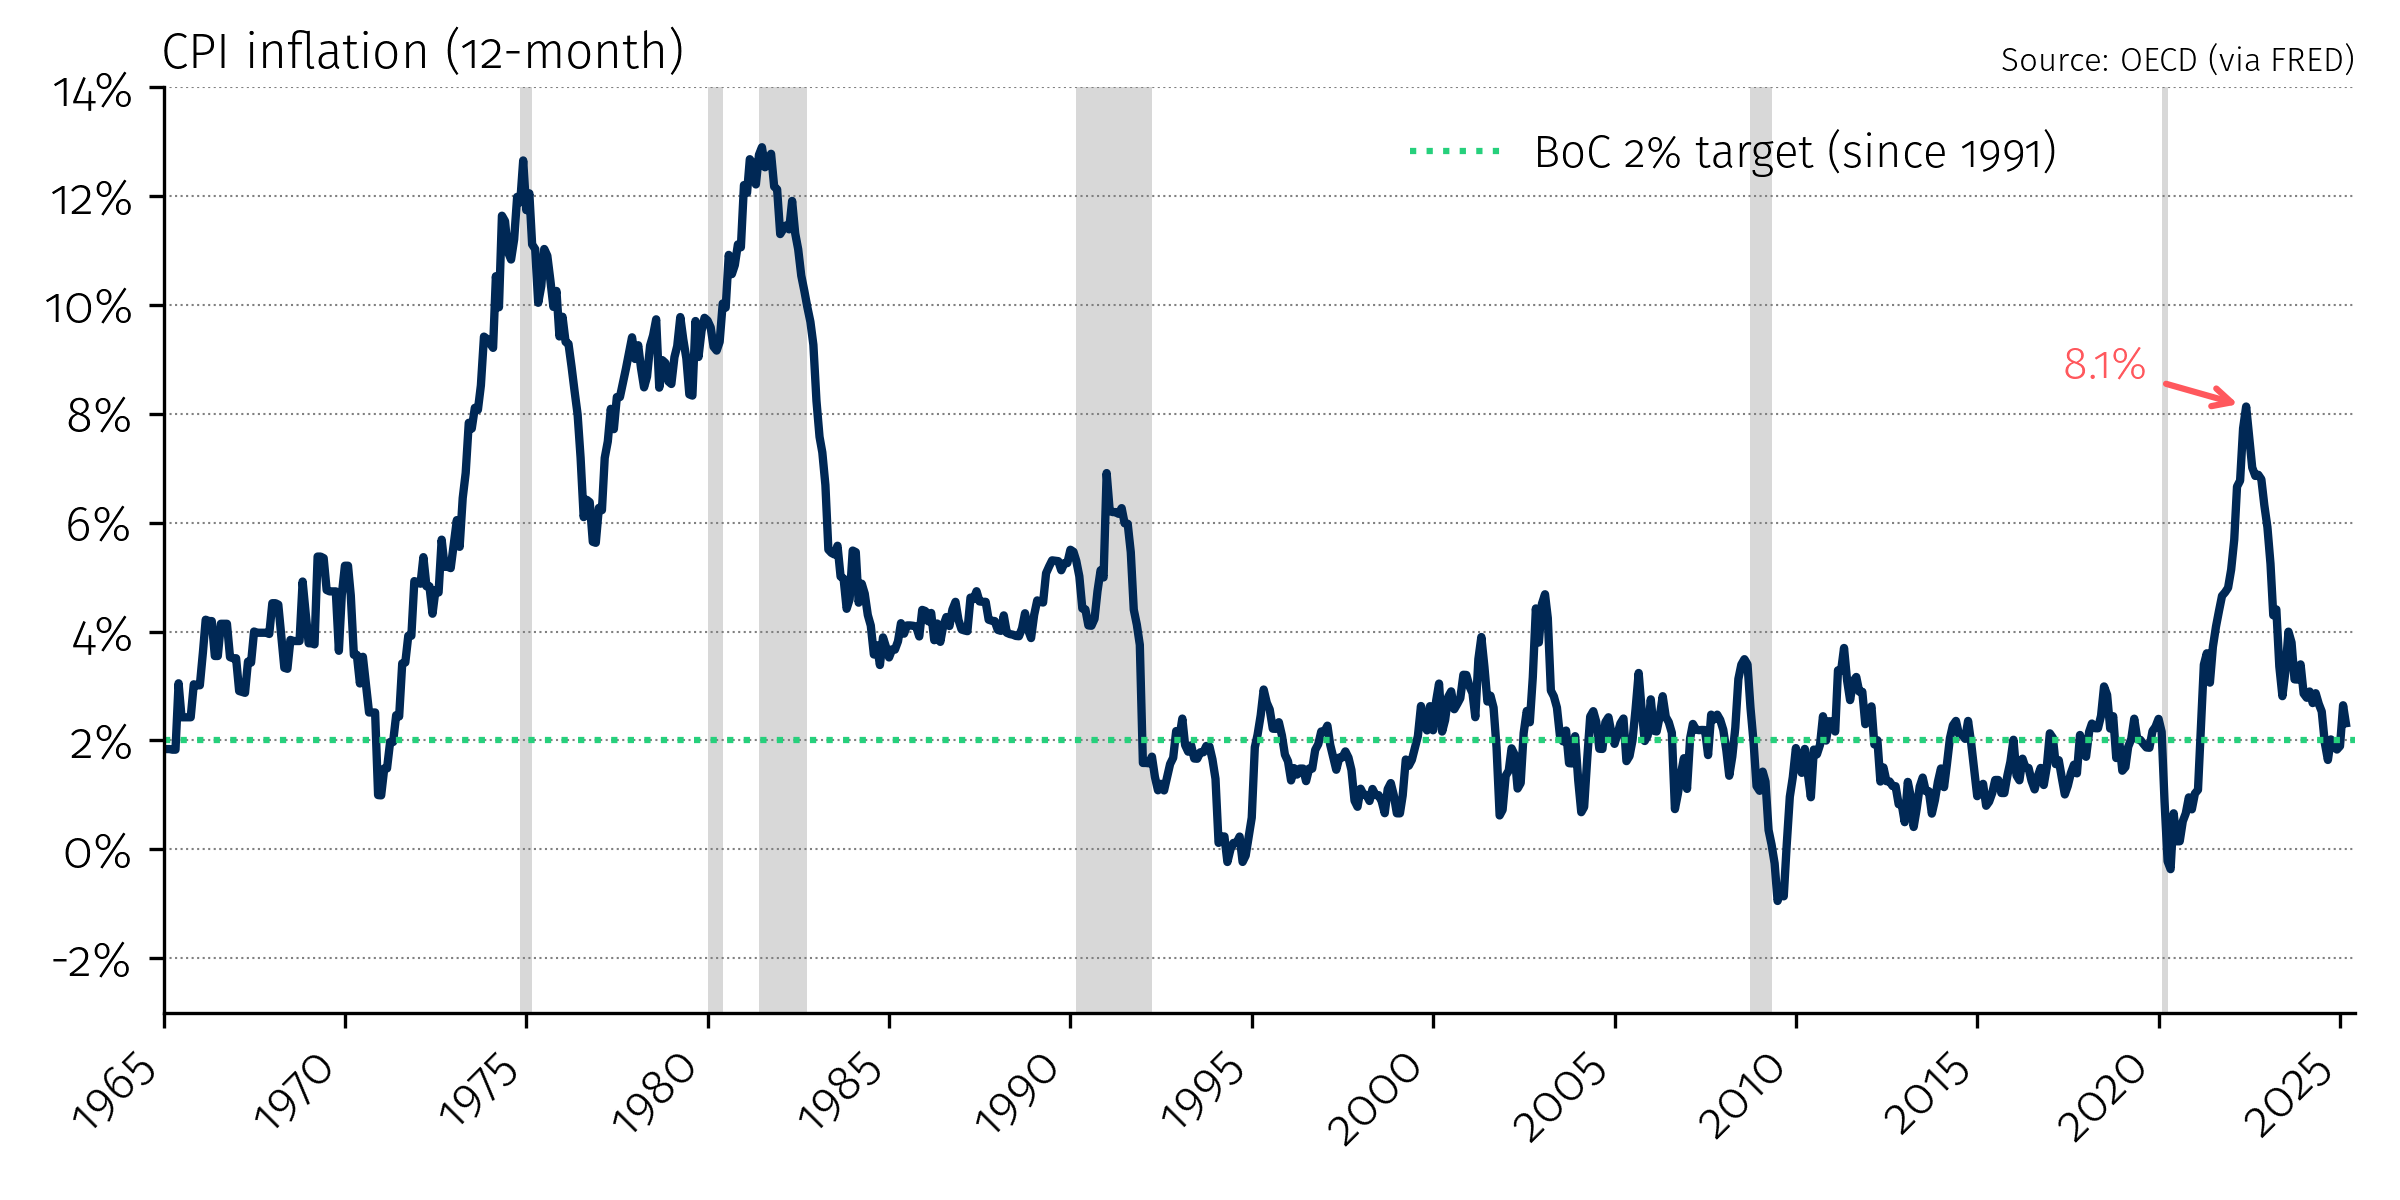
\includegraphics[width=0.9\textwidth]{can_inflation_longrun.png}
   \end{figure}
\end{frame}

% Slide N3: A forceful response...
\begin{frame}{A forceful response\ldots}
   \begin{figure}
      \centering
      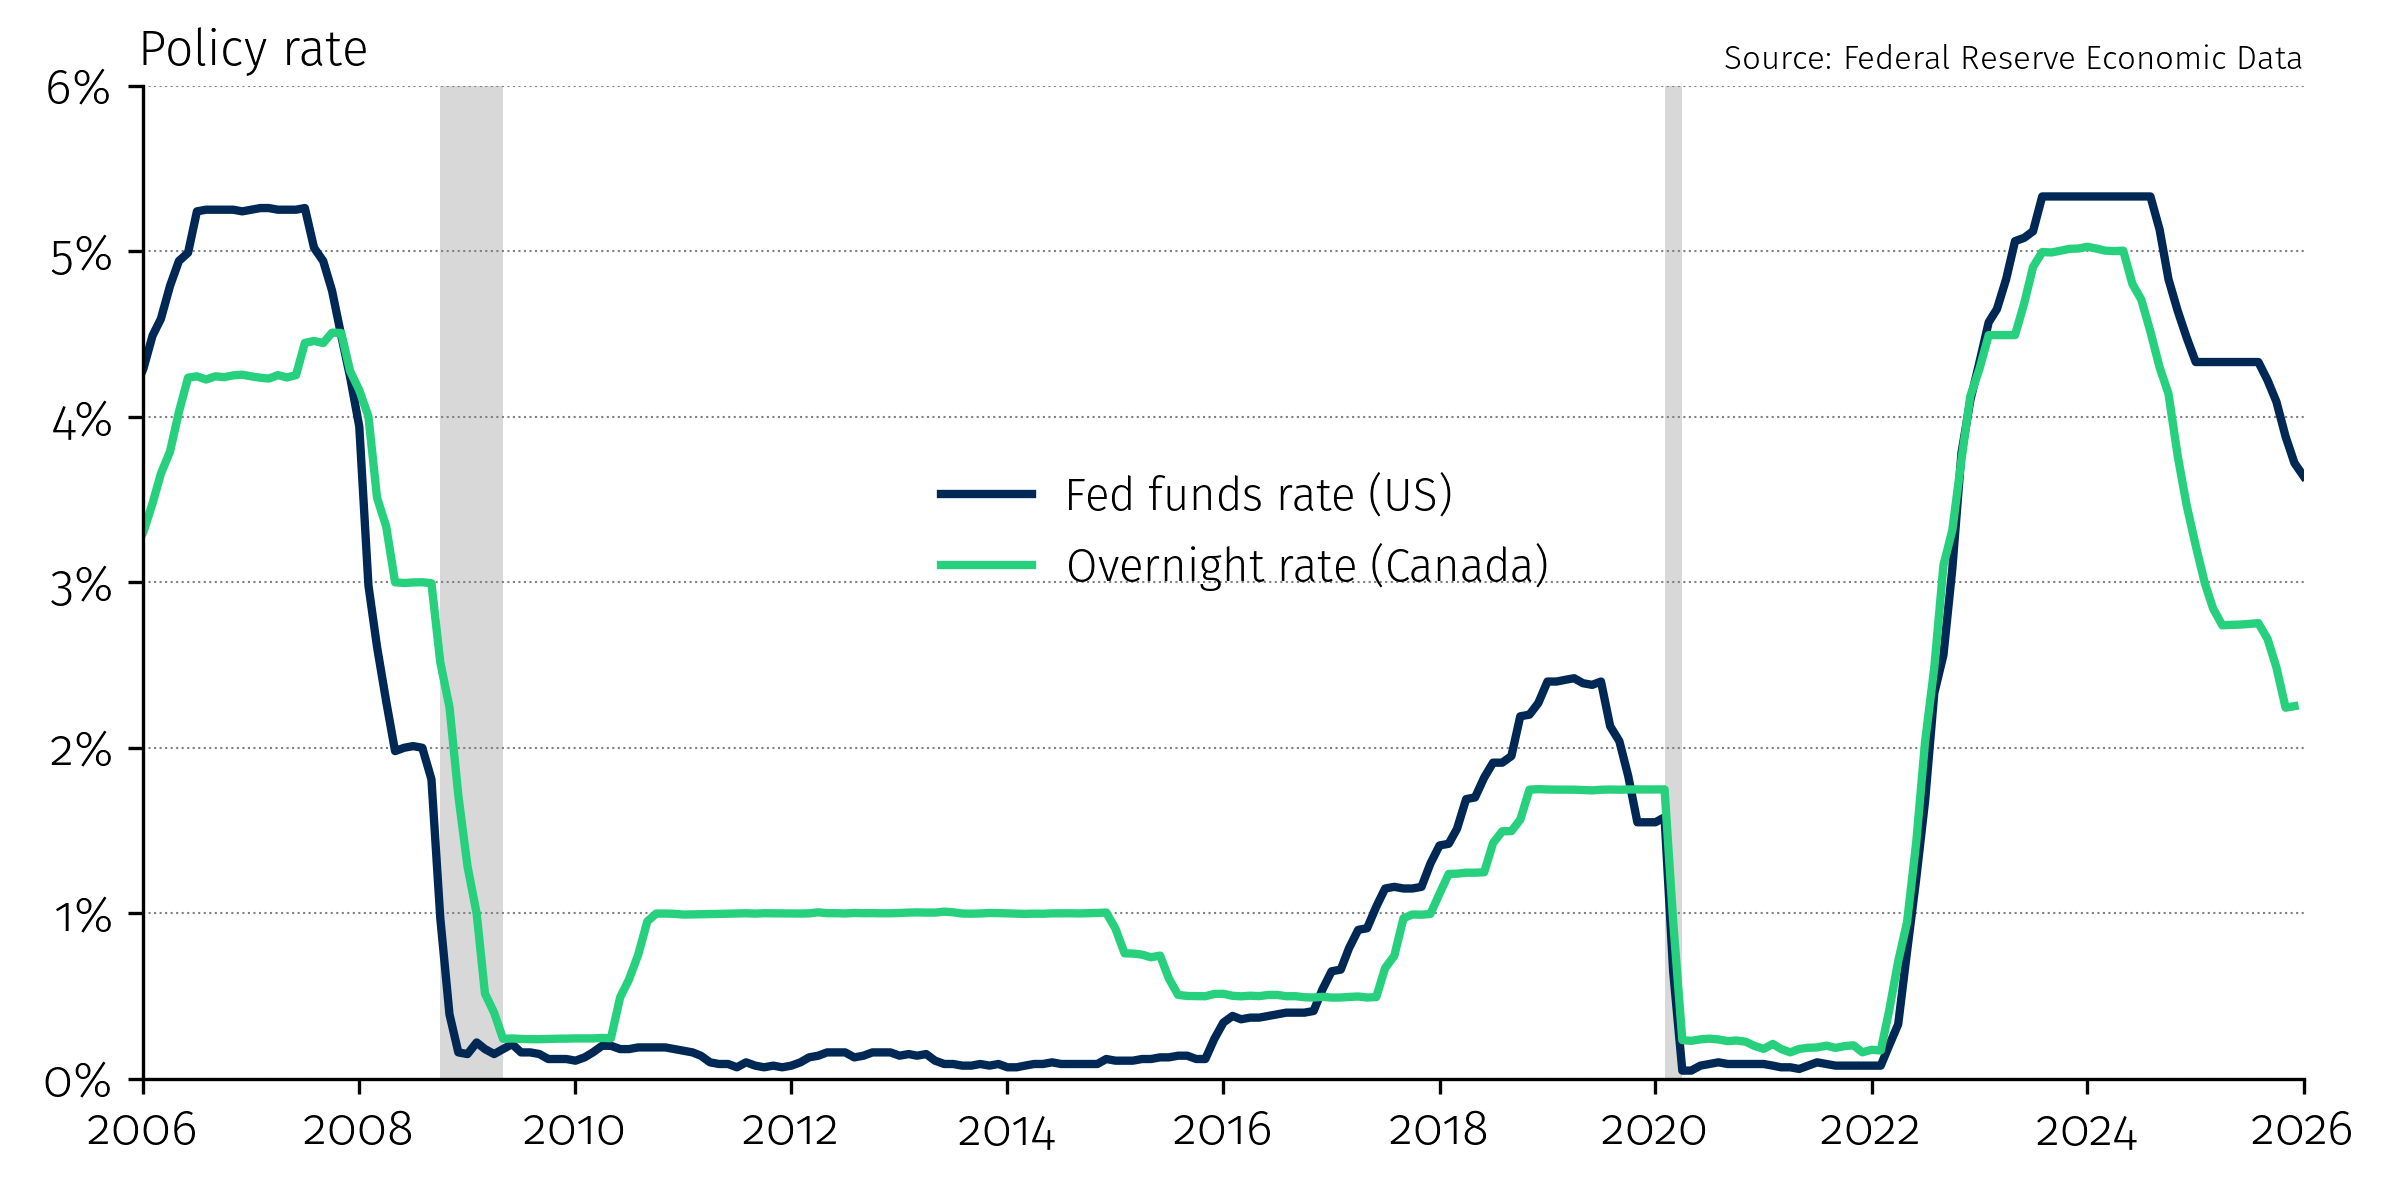
\includegraphics[width=0.9\textwidth]{policy_rates.png}
   \end{figure}
\end{frame}

% Slide N4: A return to normal...
\begin{frame}{A return to normal\ldots}
   \begin{figure}
      \centering
      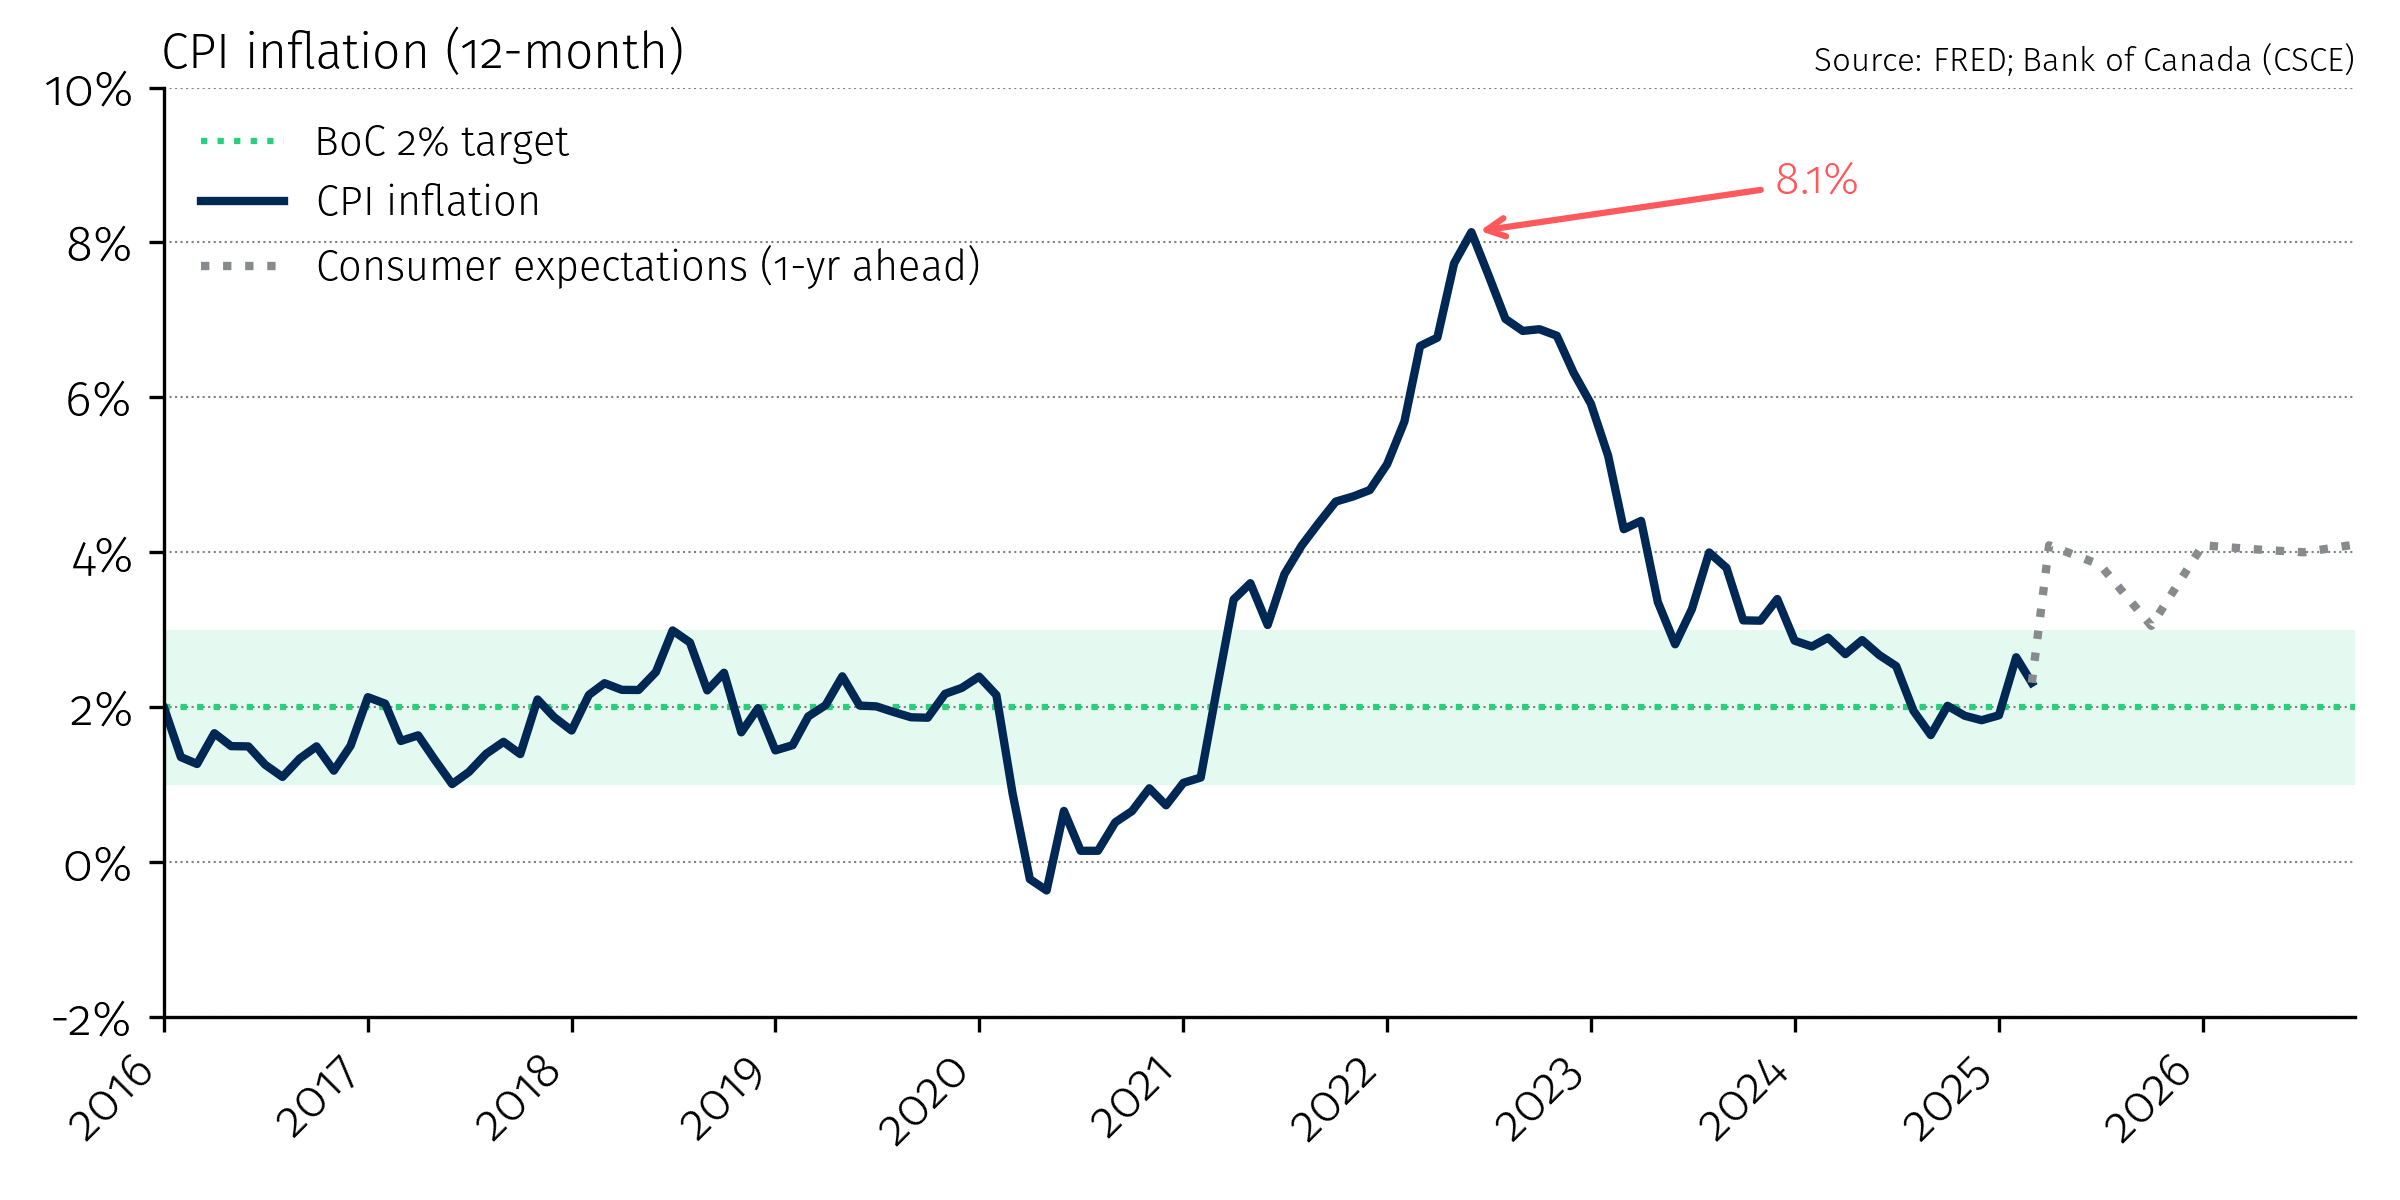
\includegraphics[width=0.9\textwidth]{canada_inflation_recent.png}
   \end{figure}
\end{frame}

% Slide N5: Trump tariffs
\begin{frame}{The return of protectionism\ldots}
   \begin{figure}
      \centering
      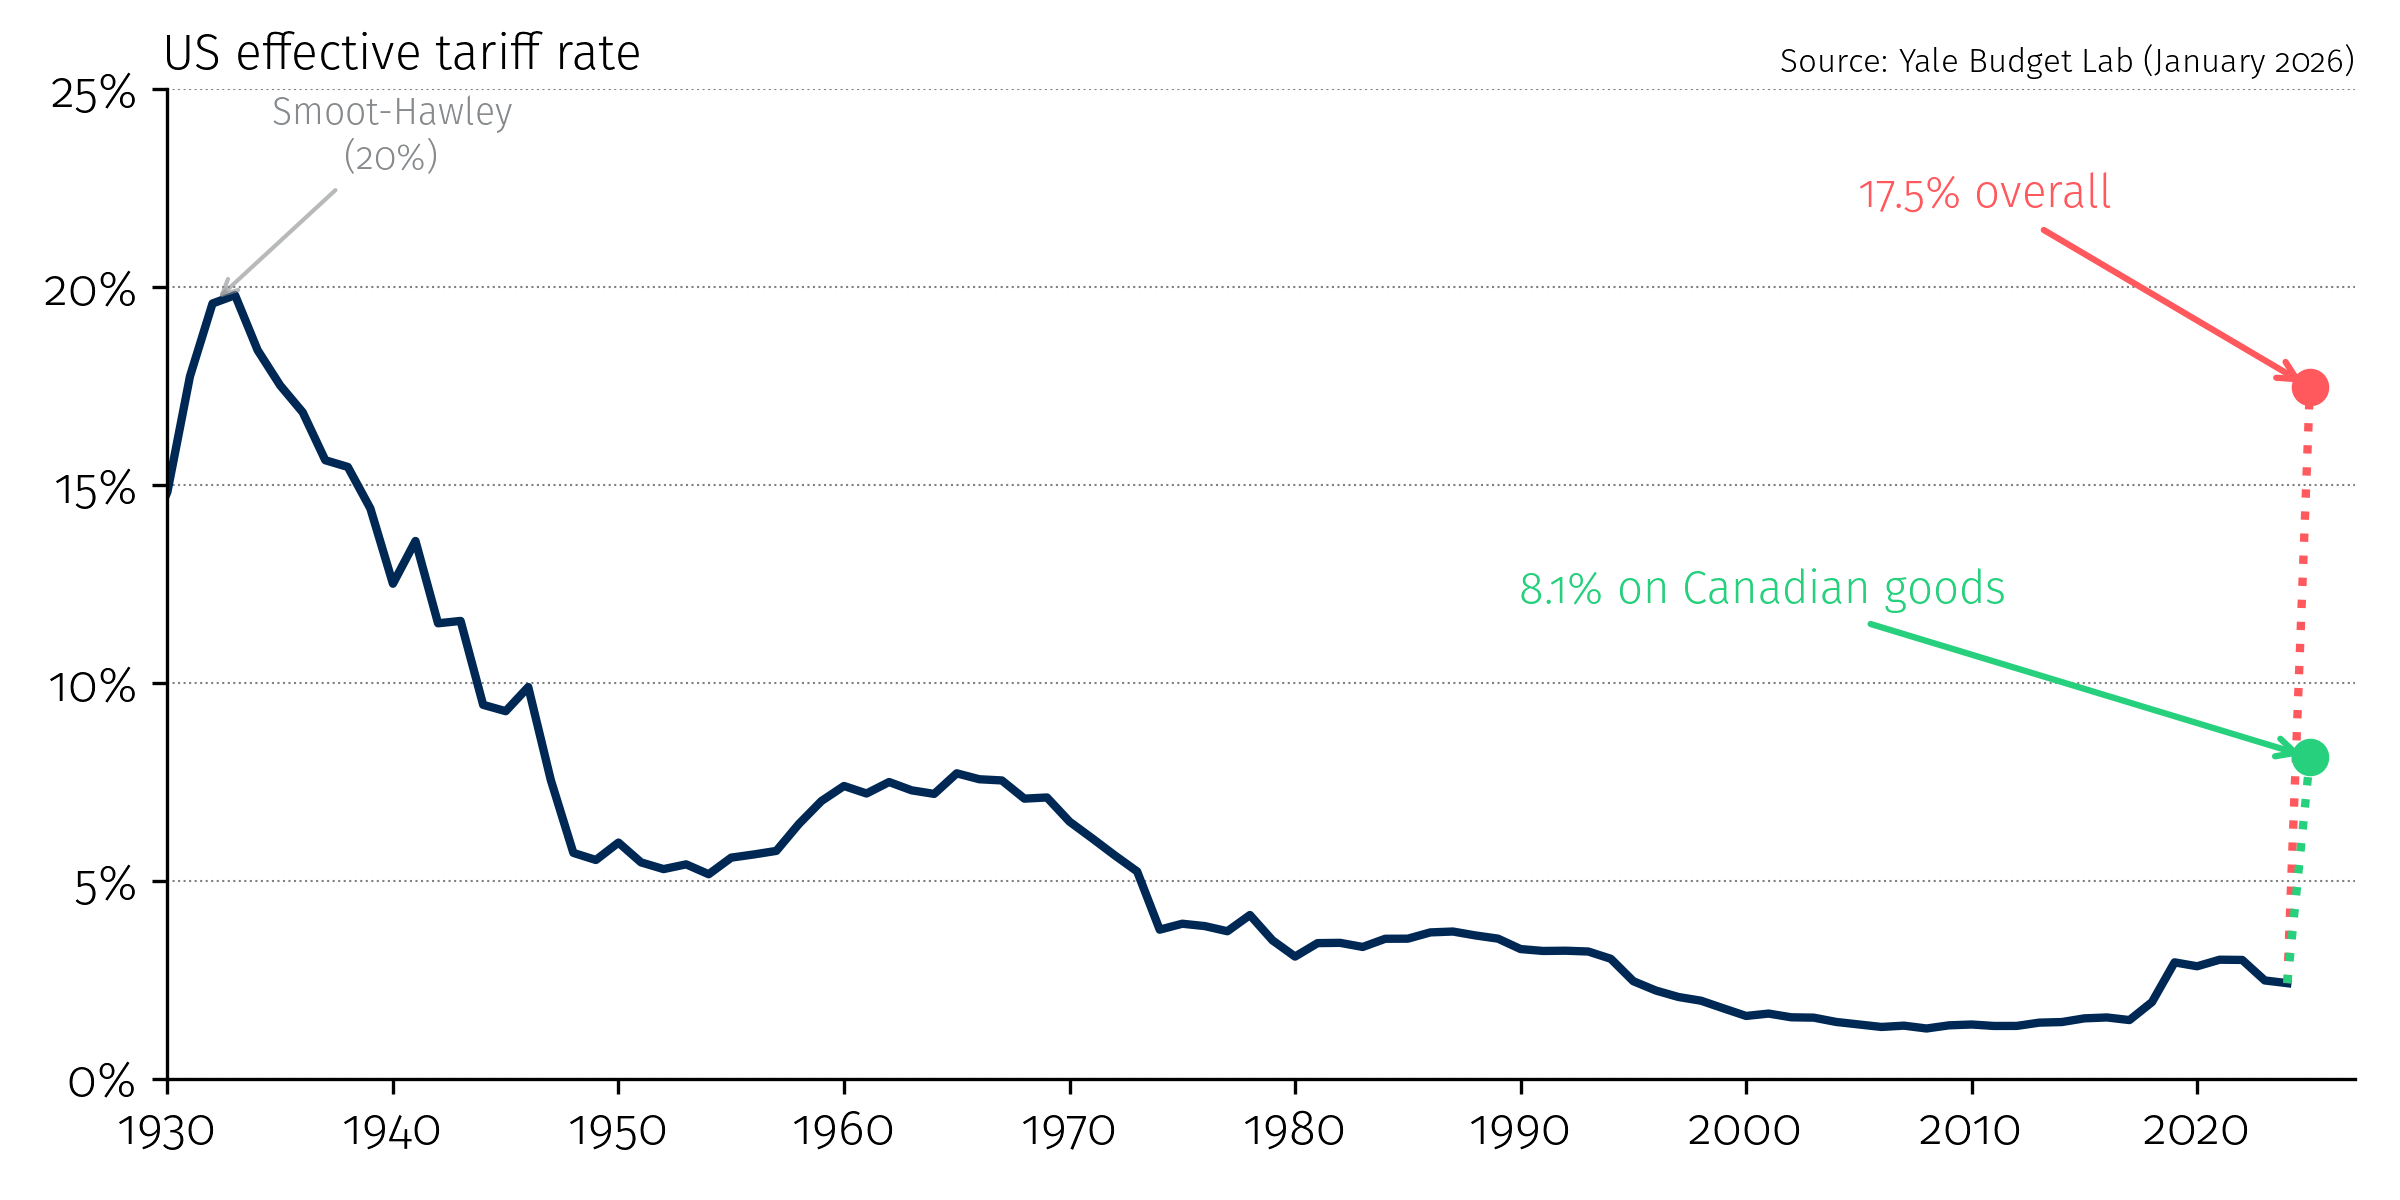
\includegraphics[width=0.9\textwidth]{us_tariff_rate.png}
   \end{figure}
\end{frame}

% Slide N6: An uncertain future...
\begin{frame}{An uncertain future\ldots}
   \begin{figure}
      \centering
      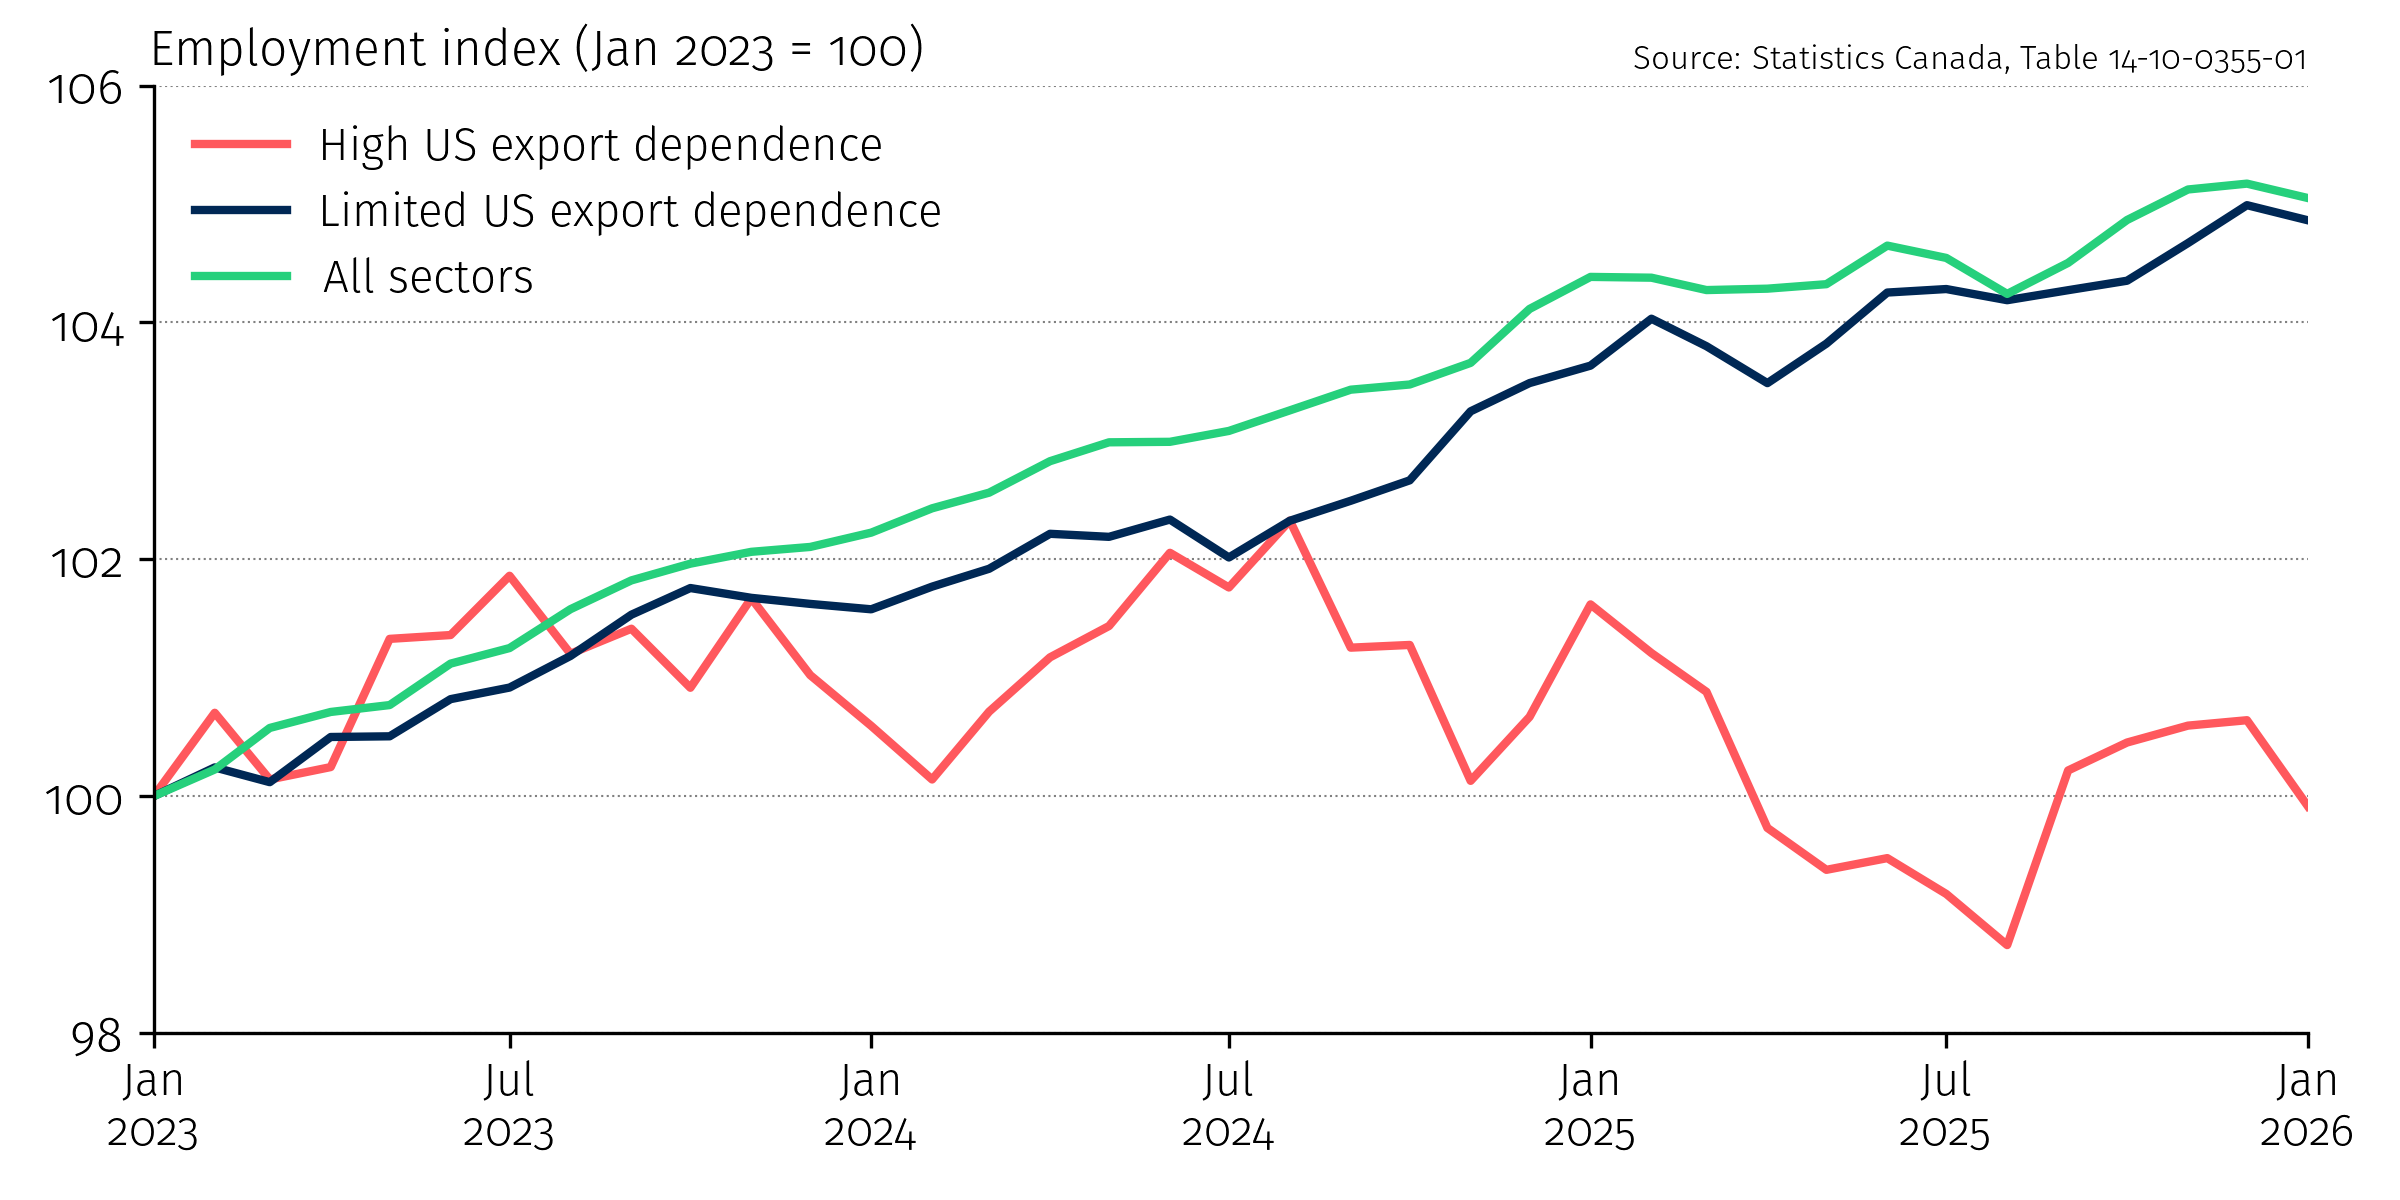
\includegraphics[width=0.9\textwidth]{canada_employment_exports.png}
   \end{figure}
\end{frame}

% Slide N6: What about the distant future?
\begin{frame}{What about the distant future?}
   \begin{figure}
      \centering
      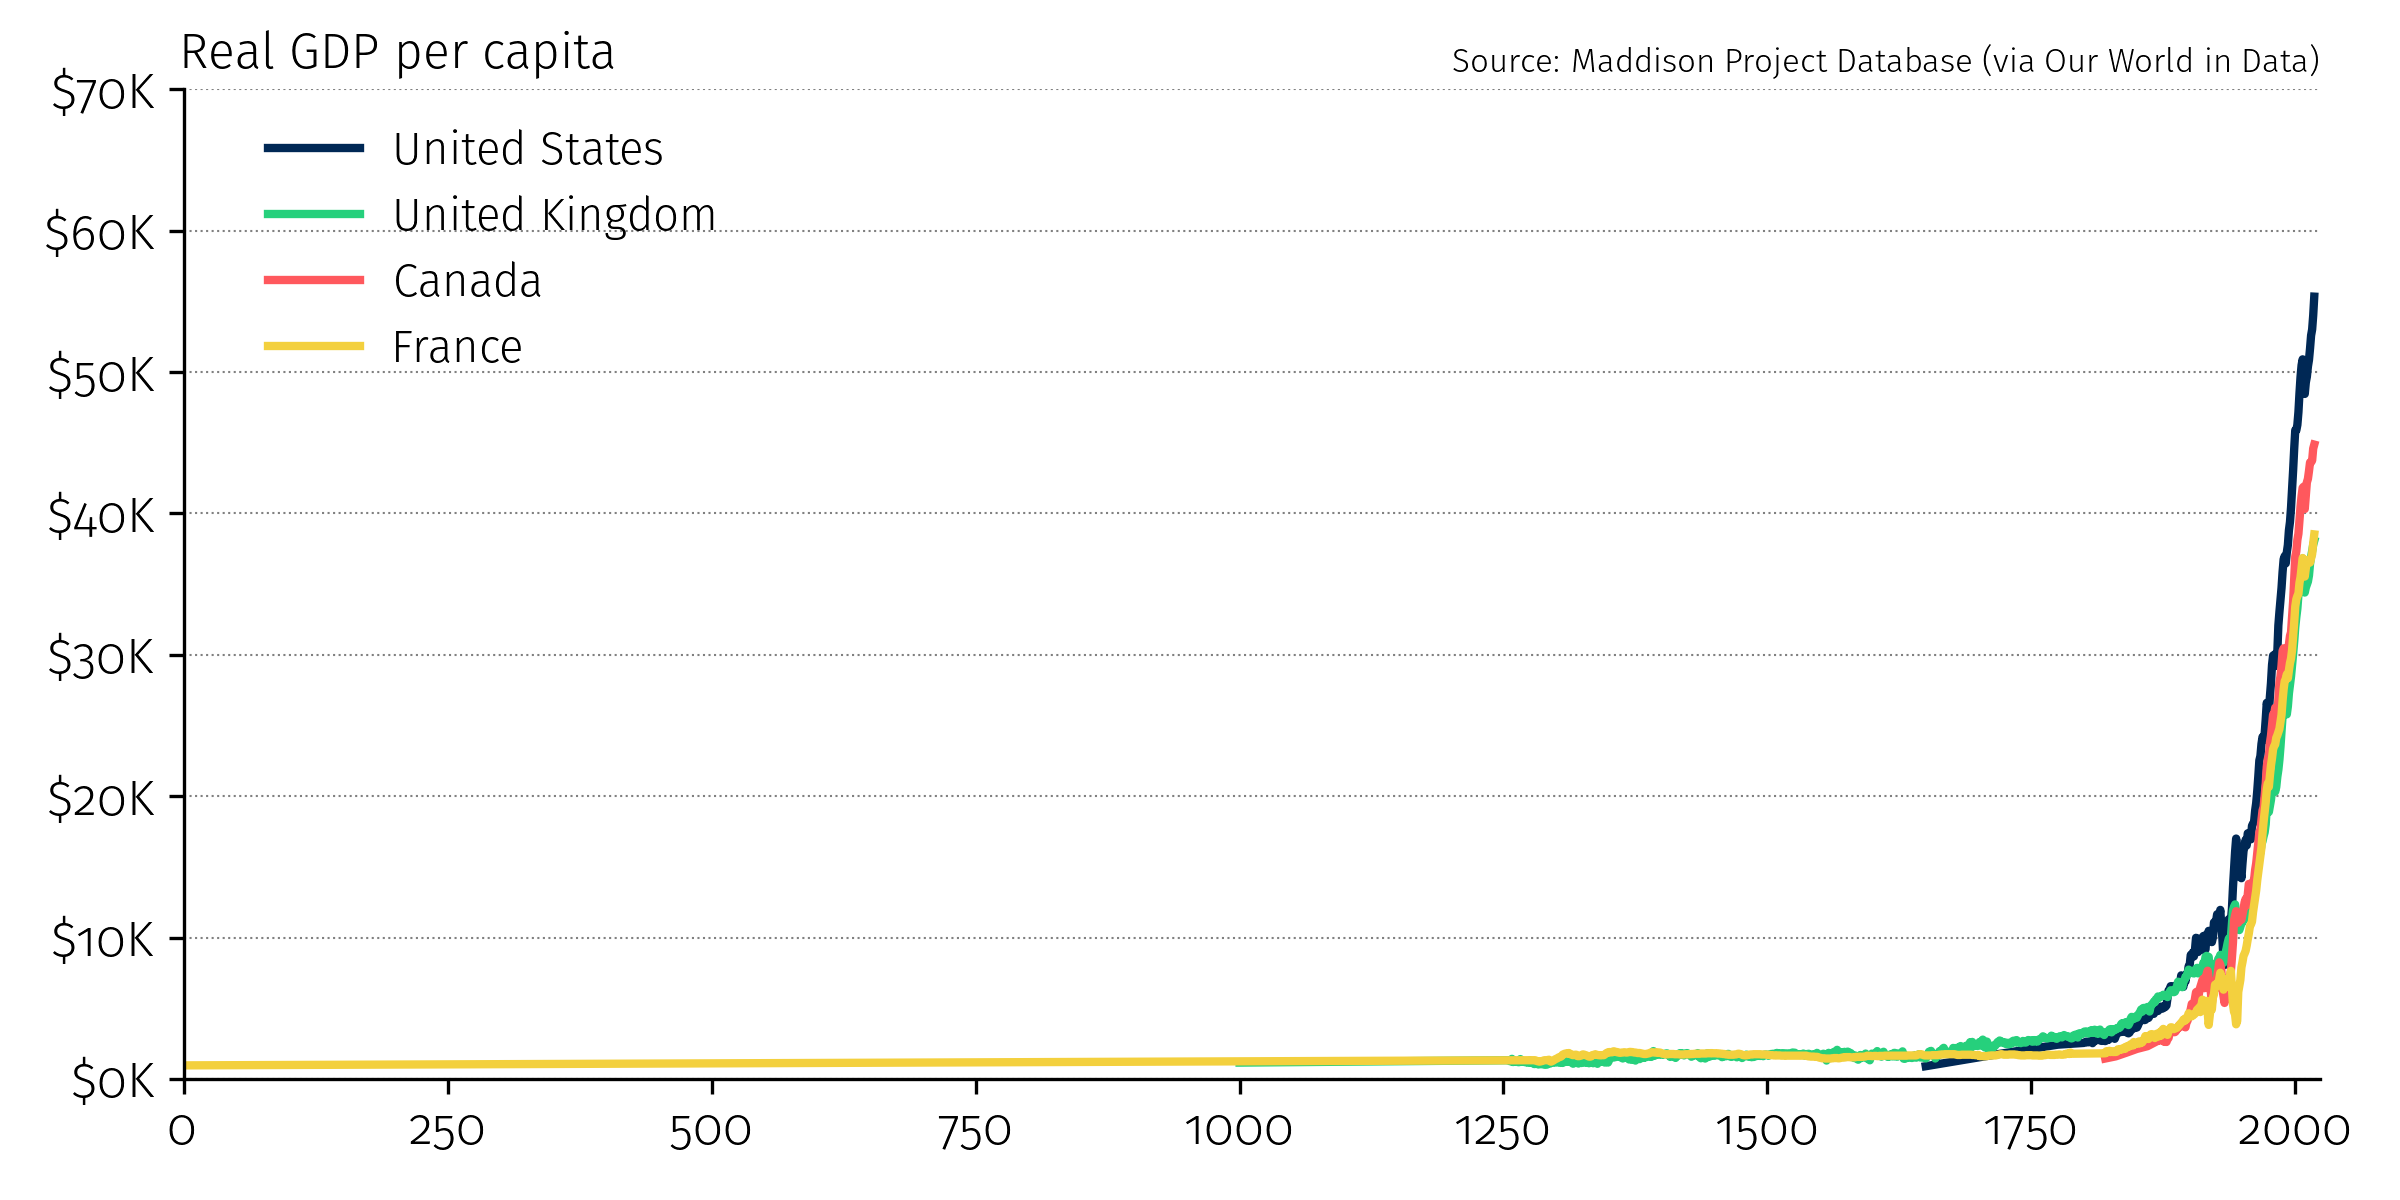
\includegraphics[width=0.9\textwidth]{hockey_stick_world.png}
   \end{figure}
\end{frame}

% ============================================================================
\begin{frame}{Outline}
   \begin{enumerate}
      \setlength\itemsep{0.35cm}
      \item \textbf{Course overview and logistics}
      \item Measuring the economy: GDP
      \item Measuring inflation
      \item Comparing living standards across countries
      \item Beyond GDP
      \item The macroeconomic landscape in 2026
   \end{enumerate}
\end{frame}

% ============================================================================
\sectionframe{Course overview}
% ============================================================================

\begin{frame}{Course objectives}
   \textbf{No, I will not make you economists\ldots but by the end of this course, you will:}
   \vspace{0.3cm}
   \begin{enumerate}
      \setlength\itemsep{0.3cm}
      \item Be \textbf{less intimidated} by macroeconomic discussions and jargon
      \item Be able to critically interpret \textbf{macroeconomic news} (``BS'' detector)
      \item Be aware of major \textbf{macroeconomic trends}
      \item Have \textbf{objective and coherent} conversations about macroeconomics
   \end{enumerate}
   \vspace{0.5cm}
   \begin{defbox}[What this course is \textbf{not}]
      Technical. Abstract. Ideological.
   \end{defbox}
\end{frame}

\begin{frame}{Themes to be covered}
   \begin{enumerate}
      \setlength\itemsep{0.5cm}
      \item \textbf{Long-run economic growth:} why are some countries rich and others poor?
      \item \textbf{The labor market:} inequality, technology, and AI
      \item \textbf{Business cycles:} why does the economy boom and bust?
      \item \textbf{Monetary and fiscal policy:} how governments fight recessions
      \item \textbf{International trade and imbalances:} (de)globalization, tariffs, etc.
   \end{enumerate}
\end{frame}

\begin{frame}{Teaching team}
   \begin{columns}[c]
      \begin{column}{0.35\textwidth}
         \begin{center}
            
\includegraphics[width=1.0\textwidth]{headshot}
         \end{center}
      \end{column}
      \hspace{-1cm}
      \begin{column}{0.65\textwidth}
         \textbf{Jean-F\'elix Brouillette} \\[0.15cm]
         Assistant Professor of Applied Economics \\[0.3cm]
         {\small B.B.A.\ and M.Sc.\ in Economics, HEC Montr\'eal \\
         Ph.D.\ in Economics, Stanford University} \\[0.3cm]
         \begin{itemize}
            \setlength\itemsep{0.15cm}
            \item E-mail: {\small \href{mailto:jean-felix.brouillette@hec.ca}{jean-felix.brouillette@hec.ca}}
            \item Office hours: TBD
            \item Office: 4.148 (CSC)
         \end{itemize}
      \end{column}
   \end{columns}
\end{frame}

\begin{frame}{Pedagogical material}
   \textbf{ZoneCours (ZC)}
   \vspace{0.1cm}
   \begin{itemize}
      \setlength\itemsep{0.1cm}
      \item Slides and articles posted before each class
      \item Exercises and solutions
   \end{itemize}
   \vspace{0.3cm}
   \textbf{Textbook}
   \vspace{0.1cm}
   \begin{itemize}
      \setlength\itemsep{0.1cm}
      \item Vincent \& Yared (Pearson Revel): not mandatory
      \item ZC: reference for lectures + exercises
   \end{itemize}
   \vspace{0.3cm}
   \textbf{Stay on top of macro news}
   \vspace{0.1cm}
   \begin{itemize}
      \item \textit{The Economist, The Financial Times, The Wall Street Journal, Bloomberg, La Presse Affaires, Reuters, Les Échos, etc.}
   \end{itemize}
\end{frame}

\begin{frame}{Grades}
   \vspace{0.3cm}
   \begin{tabular}{l r}
      \textbf{Team project} (two parts) & \textbf{30\%} \\[0.2cm]
      \textbf{Quiz} (session 4, $\sim$15 minutes, multiple choice) & \textbf{10\%} \\[0.2cm]
      \textbf{Final exam} (March 30th) & \textbf{50\%} \\[0.2cm]
      \textbf{Contribution and professionalism} & \textbf{10\%} \\
   \end{tabular}
   \vspace{0.4cm}
   \begin{defbox}[Details]
      Team project details are on ZC. Examples of quiz questions will be provided.
   \end{defbox}
\end{frame}

\begin{frame}{Contribution and professionalism}
   \small
   \textbf{Criteria:}
   \vspace{0.15cm}
   \begin{enumerate}
      \setlength\itemsep{0.2cm}
      \item \textbf{Attendance and punctuality} --- as per program requirements
      \item \textbf{Active participation} --- quality and relevance of interventions
      \item \textbf{Professionalism} --- autonomy, judgment, collegiality
   \end{enumerate}
   \vspace{0.4cm}
   \textbf{To promote active learning:}
   \vspace{0.15cm}
   \begin{enumerate}
      \setlength\itemsep{0.2cm}
      \item \textbf{Name cards} --- please bring yours to every class
      \item \textbf{No laptops} in class (exception: tablets lying flat)
      \item \textbf{Limit comings and goings} during class
   \end{enumerate}
\end{frame}

% ============================================================================
\begin{frame}{Outline}
   \begin{enumerate}
      \setlength\itemsep{0.35cm}
      \item {\color{gray!50}Course overview and logistics}
      \item \textbf{Measuring the economy: GDP}
      \item Measuring inflation
      \item Comparing living standards across countries
      \item Beyond GDP
      \item The macroeconomic landscape in 2026
   \end{enumerate}
\end{frame}

% ============================================================================
\sectionframe{Measuring the economy: GDP}
% ============================================================================

\begin{frame}{What is GDP?}
   \begin{defbox}[Gross Domestic Product (GDP)]
      The total \textbf{market value} of all \textbf{final} goods and services produced \textbf{within a country} during a \textbf{given period}.
   \end{defbox}
   \vspace{0.3cm}
   \textbf{Key words:}
   \vspace{0.15cm}
   \begin{itemize}
      \setlength\itemsep{0.15cm}
      \item \textbf{Market value:} measured in dollars (or another currency)
      \item \textbf{Final:} excludes intermediate goods to avoid double-counting
      \item \textbf{Within a country:} production on Canadian soil
      \item \textbf{Given period:} a flow, not a stock (typically quarterly or annual)
   \end{itemize}
\end{frame}

\begin{frame}[t]{Three ways to measure GDP}
   \framesubtitle{They all give the same answer}

   \small
   \noindent%
   \begin{minipage}[t]{0.33\textwidth}
      \textbf{\textcolor{HECnavy}{1. Expenditure}}\\[4pt]
      Who is buying?
      \vspace{-0.2cm}
      \begin{equation*}
         Y = C + I + G + NX
      \end{equation*}
      \vspace{-0.8cm}
      \begin{itemize}
         \footnotesize
         \item $C$: consumption
         \item $I$: investment
         \item $G$: gov. spending
         \item $NX$: net exports
      \end{itemize}
   \end{minipage}%
   \begin{minipage}[t]{0.33\textwidth}
      \textbf{\textcolor{HECnavy}{2. Income}}\\[4pt]
      Who is earning?
      \vspace{0.1cm}
      \begin{itemize}
         \footnotesize
         \item Wages/salaries
         \item Corporate profits
         \item Rental income
         \item Interest income
      \end{itemize}
   \end{minipage}%
   \hspace{-0.5cm}
   \begin{minipage}[t]{0.33\textwidth}
      \textbf{\textcolor{HECnavy}{3. Value added}}\\[4pt]
      Who is producing?
      \vspace{0.1cm}
      \begin{itemize}
         \footnotesize
         \item Value added at each stage
         \item Revenue $-$ int. inputs
      \end{itemize}
   \end{minipage}
   \vspace{0.1cm}
   \begin{keyinsight}
      Every dollar spent is a dollar earned is a dollar of value created
   \end{keyinsight}
\end{frame}

\begin{frame}[t]{Example: value added avoids double counting}
   \footnotesize
   \begin{tcolorbox}[
      colback=white, colframe=HECnavy, colbacktitle=HECnavy,
      title=\textbf{Example}, fonttitle=\footnotesize, boxrule=0.5pt, arc=8pt,
      top=3pt, bottom=3pt, left=6pt, right=6pt
   ]
      A business hires employees to work in a fertilizer plant and pays them \$0.50 in wages. The business sells the fertilizer to Dwight, a self-employed farmer, for \$0.80. Dwight uses it to produce beets, which he sells to Jim for \$1. Jim eats the beets.
      \vspace{0.1cm}

      \renewcommand{\arraystretch}{1.1}
      \centering
      \begin{tabularx}{\linewidth}{X r >{\hspace{0.15cm}}X r >{\hspace{0.15cm}}X r}
         \rowcolor{HECnavy!10}
         \textbf{Production} & & \textbf{Income} & & \textbf{Expenditure} & \\
         \hline
         Manufacturing & 0.80 & Wages & 0.50 & Consumption & 1.00 \\
         Agriculture & 0.20 & Profits & 0.30 & & \\
         & & Prop.\ income & 0.20 & & \\
         \hline
         \textbf{Total} & \textbf{1.00} & \textbf{Total} & \textbf{1.00} & \textbf{Total} & \textbf{1.00}
      \end{tabularx}
   \end{tcolorbox}
   \vspace{0.05cm}
   \begin{keyinsight}
      Production = \textbf{value added} (revenue $-$ intermediate inputs), not total revenue. This avoids double counting and ensures all three approaches agree.
   \end{keyinsight}
\end{frame}

\begin{frame}{The expenditure approach: $Y = C + I + G + NX$}
   \begin{figure}
      \centering
      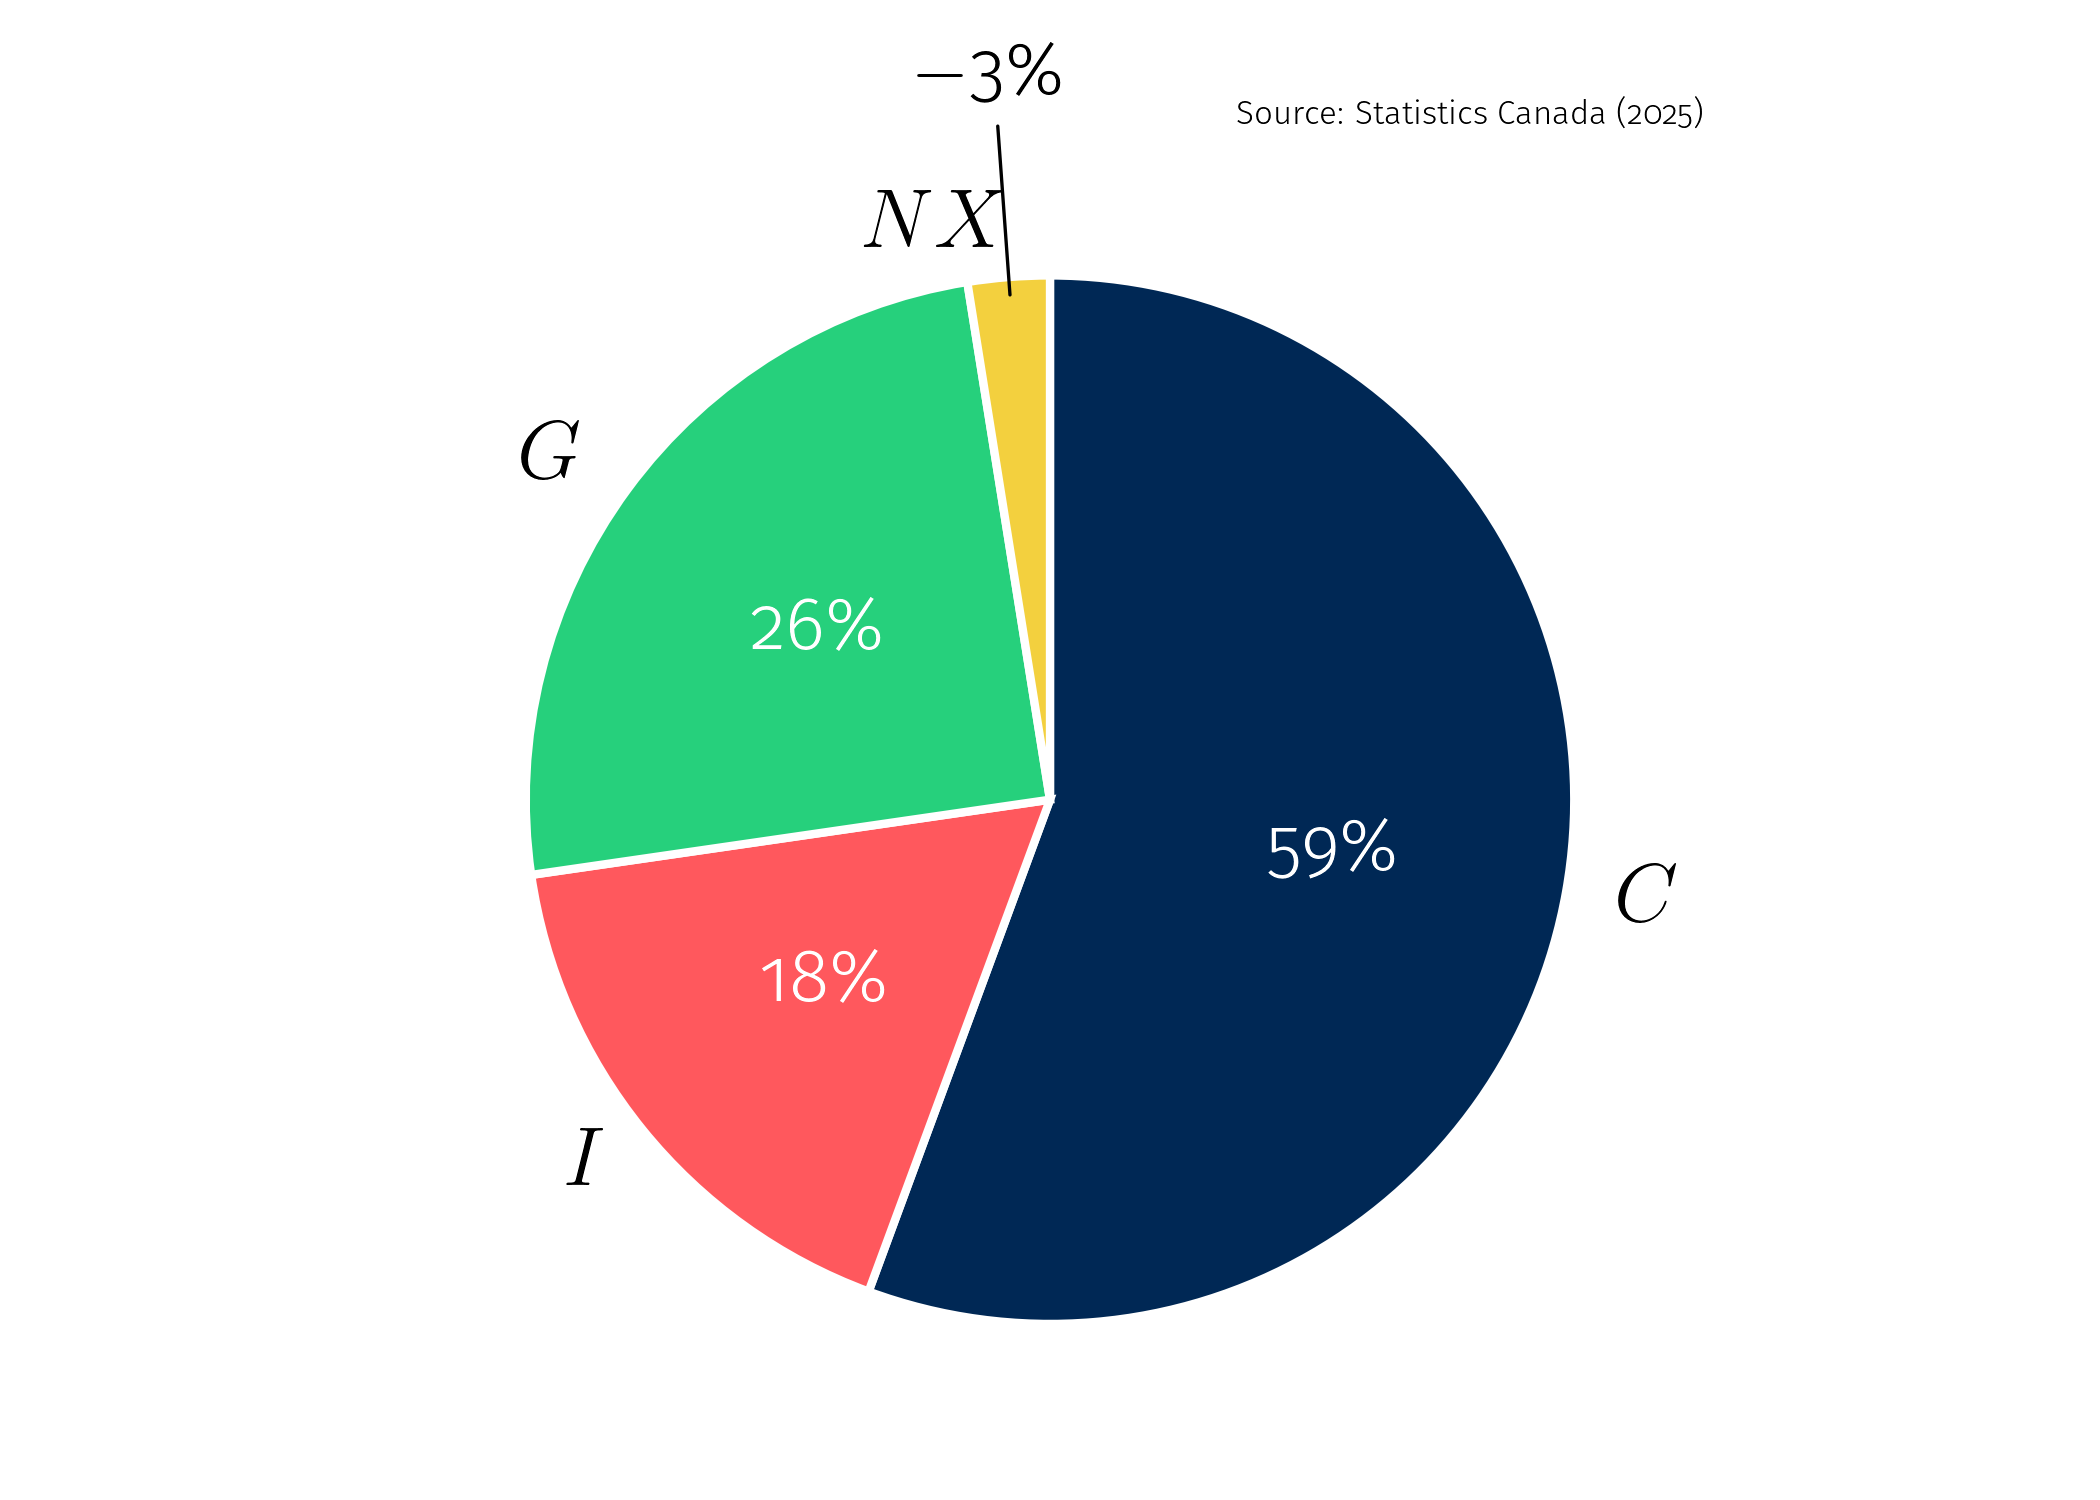
\includegraphics[height=0.8\textheight]{gdp_decomposition_canada.png}
   \end{figure}
\end{frame}

% ── Consumption ───────────────────────────────────────────────────────

\begin{frame}[t]{Consumption ($C$)}
   \textbf{Household spending} on final goods and services:
   \vspace{0.2cm}
   \begin{itemize}
      \setlength\itemsep{0.15cm}
      \item \textbf{Durable goods} --- cars, furniture, appliances (long-lasting)
      \item \textbf{Non-durable goods} --- food, clothing, gasoline (used up quickly)
      \item \textbf{Services} --- rent, healthcare, haircuts, education
   \end{itemize}
   \vspace{0.3cm}
   \begin{keyinsight}
      Services account for over 60\% of consumption in Canada. The shift from goods to services is a hallmark of advanced economies.
   \end{keyinsight}
\end{frame}

\begin{frame}{Consumption share of GDP in Canada}
   \vspace{-0.2cm}
   \begin{figure}
      \centering
      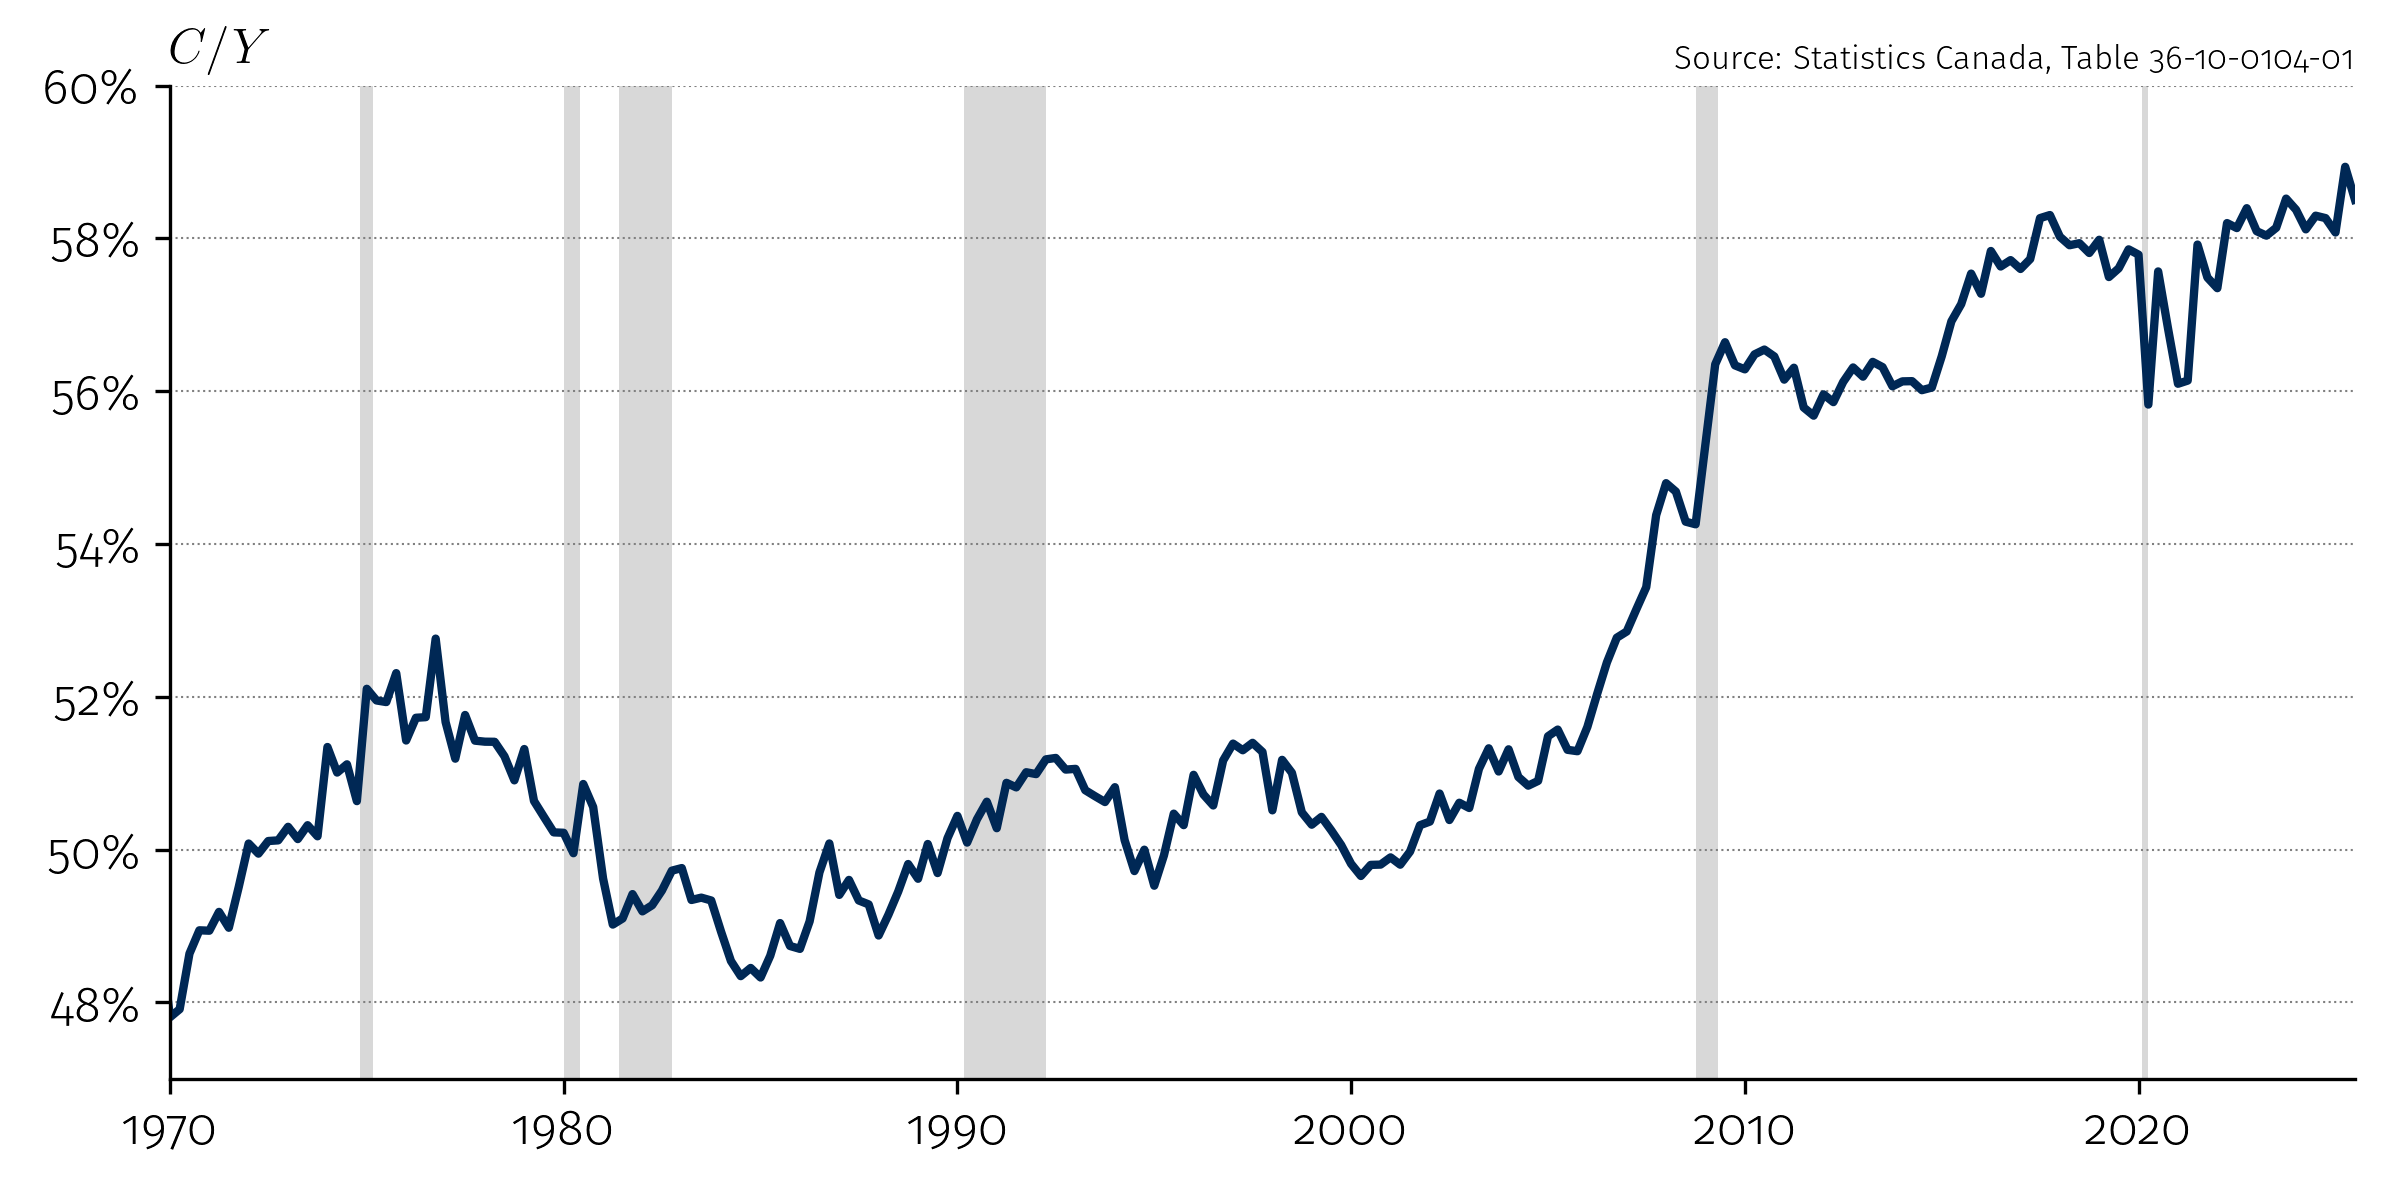
\includegraphics[width=0.95\textwidth]{consumption_share_gdp.png}
   \end{figure}
   \vspace{-0.4cm}
   \footnotesize Consumption is the largest component ($\approx$60\%), and increasing over time.
\end{frame}

% ── Investment ────────────────────────────────────────────────────────

\begin{frame}[t]{Investment ($I$)}
   \textbf{Spending on goods used to produce future output:}
   \vspace{0.2cm}
   \begin{itemize}
      \setlength\itemsep{0.15cm}
      \item \textbf{Business fixed capital} --- machines, equipment, factories, software
      \item \textbf{Residential} --- new housing construction
      \item \textbf{Inventories} --- unsold goods stored in warehouses
   \end{itemize}
   \vspace{0.3cm}
   \begin{warning}[Common confusion]
      In economics, ``investment'' means \textbf{physical capital formation}, not buying stocks or bonds. A firm purchasing a delivery van is investment; buying shares of Tesla is not.
   \end{warning}
\end{frame}

\begin{frame}[t]{Example: investment}
   \footnotesize
   \begin{tcolorbox}[
      colback=white, colframe=HECnavy, colbacktitle=HECnavy,
      title=\textbf{Example}, fonttitle=\footnotesize, boxrule=0.5pt, arc=8pt,
      top=3pt, bottom=3pt, left=6pt, right=6pt
   ]
      General Motors produces a minivan, which it sells for \$1,000 to the Michael Scott Paper Company. The cost of producing it is made up of workers' wages worth \$600.
      \vspace{0.1cm}

      \renewcommand{\arraystretch}{1.1}
      \centering
      \begin{tabularx}{\linewidth}{X r >{\hspace{0.15cm}}X r >{\hspace{0.15cm}}X r}
         \rowcolor{HECnavy!10}
         \textbf{Production} & & \textbf{Income} & & \textbf{Expenditure} & \\
         \hline
         Manufacturing & 1,000 & Wages & 600 & Investment & 1,000 \\
         & & Profits & 400 & & \\
         \hline
         \textbf{Total} & \textbf{1,000} & \textbf{Total} & \textbf{1,000} & \textbf{Total} & \textbf{1,000}
      \end{tabularx}
   \end{tcolorbox}
   \vspace{0.05cm}
   \begin{keyinsight}
      A firm buying a capital good = \textbf{investment}, not consumption.
   \end{keyinsight}
\end{frame}

\begin{frame}[t]{Example: inventories (Year 1)}
   \footnotesize
   \begin{tcolorbox}[
      colback=white, colframe=HECnavy, colbacktitle=HECnavy,
      title=\textbf{Example}, fonttitle=\footnotesize, boxrule=0.5pt, arc=8pt,
      top=3pt, bottom=3pt, left=6pt, right=6pt
   ]
      Dunder Mifflin produces 500 tons of white paper worth \$400 and stores them in its warehouse while it waits for customers to buy them. The cost of producing them is made up of workers' wages of \$500.
      \vspace{0.1cm}

      \renewcommand{\arraystretch}{1.1}
      \centering
      \begin{tabularx}{\linewidth}{X r >{\hspace{0.15cm}}X r >{\hspace{0.15cm}}X r}
         \rowcolor{HECnavy!10}
         \textbf{Production} & & \textbf{Income} & & \textbf{Expenditure} & \\
         \hline
         Manufacturing & 400 & Wages & 500 & Investment & 400 \\
         & & Profits & (100) & & \\
         \hline
         \textbf{Total} & \textbf{400} & \textbf{Total} & \textbf{400} & \textbf{Total} & \textbf{400}
      \end{tabularx}
   \end{tcolorbox}
   \vspace{0.05cm}
   \begin{keyinsight}
      Unsold goods = \textbf{inventory investment}. GDP captures all production, even without a sale.
   \end{keyinsight}
\end{frame}

\begin{frame}[t]{Example: inventories (Year 2)}
   \footnotesize
   \begin{tcolorbox}[
      colback=white, colframe=HECnavy, colbacktitle=HECnavy,
      title=\textbf{Example}, fonttitle=\footnotesize, boxrule=0.5pt, arc=8pt,
      top=3pt, bottom=3pt, left=6pt, right=6pt
   ]
      The following year, Dunder Mifflin finally sells its paper worth \$400.
      \vspace{0.1cm}

      \renewcommand{\arraystretch}{1.1}
      \centering
      \begin{tabularx}{\linewidth}{X r >{\hspace{0.15cm}}X r >{\hspace{0.15cm}}X r}
         \rowcolor{HECnavy!10}
         \textbf{Production} & & \textbf{Income} & & \textbf{Expenditure} & \\
         \hline
         & & & & Consumption & 400 \\
         & & & & Investment & (400) \\
         \hline
         \textbf{Total} & \textbf{0} & \textbf{Total} & \textbf{0} & \textbf{Total} & \textbf{0}
      \end{tabularx}
   \end{tcolorbox}
   \vspace{0.05cm}
   \begin{keyinsight}
      Selling from inventory: $C$ rises, $I$ falls $\Rightarrow$ GDP = 0. Production was counted in year~1.
   \end{keyinsight}
\end{frame}

\begin{frame}{Investment share of GDP in Canada}
   \vspace{-0.2cm}
   \begin{figure}
      \centering
      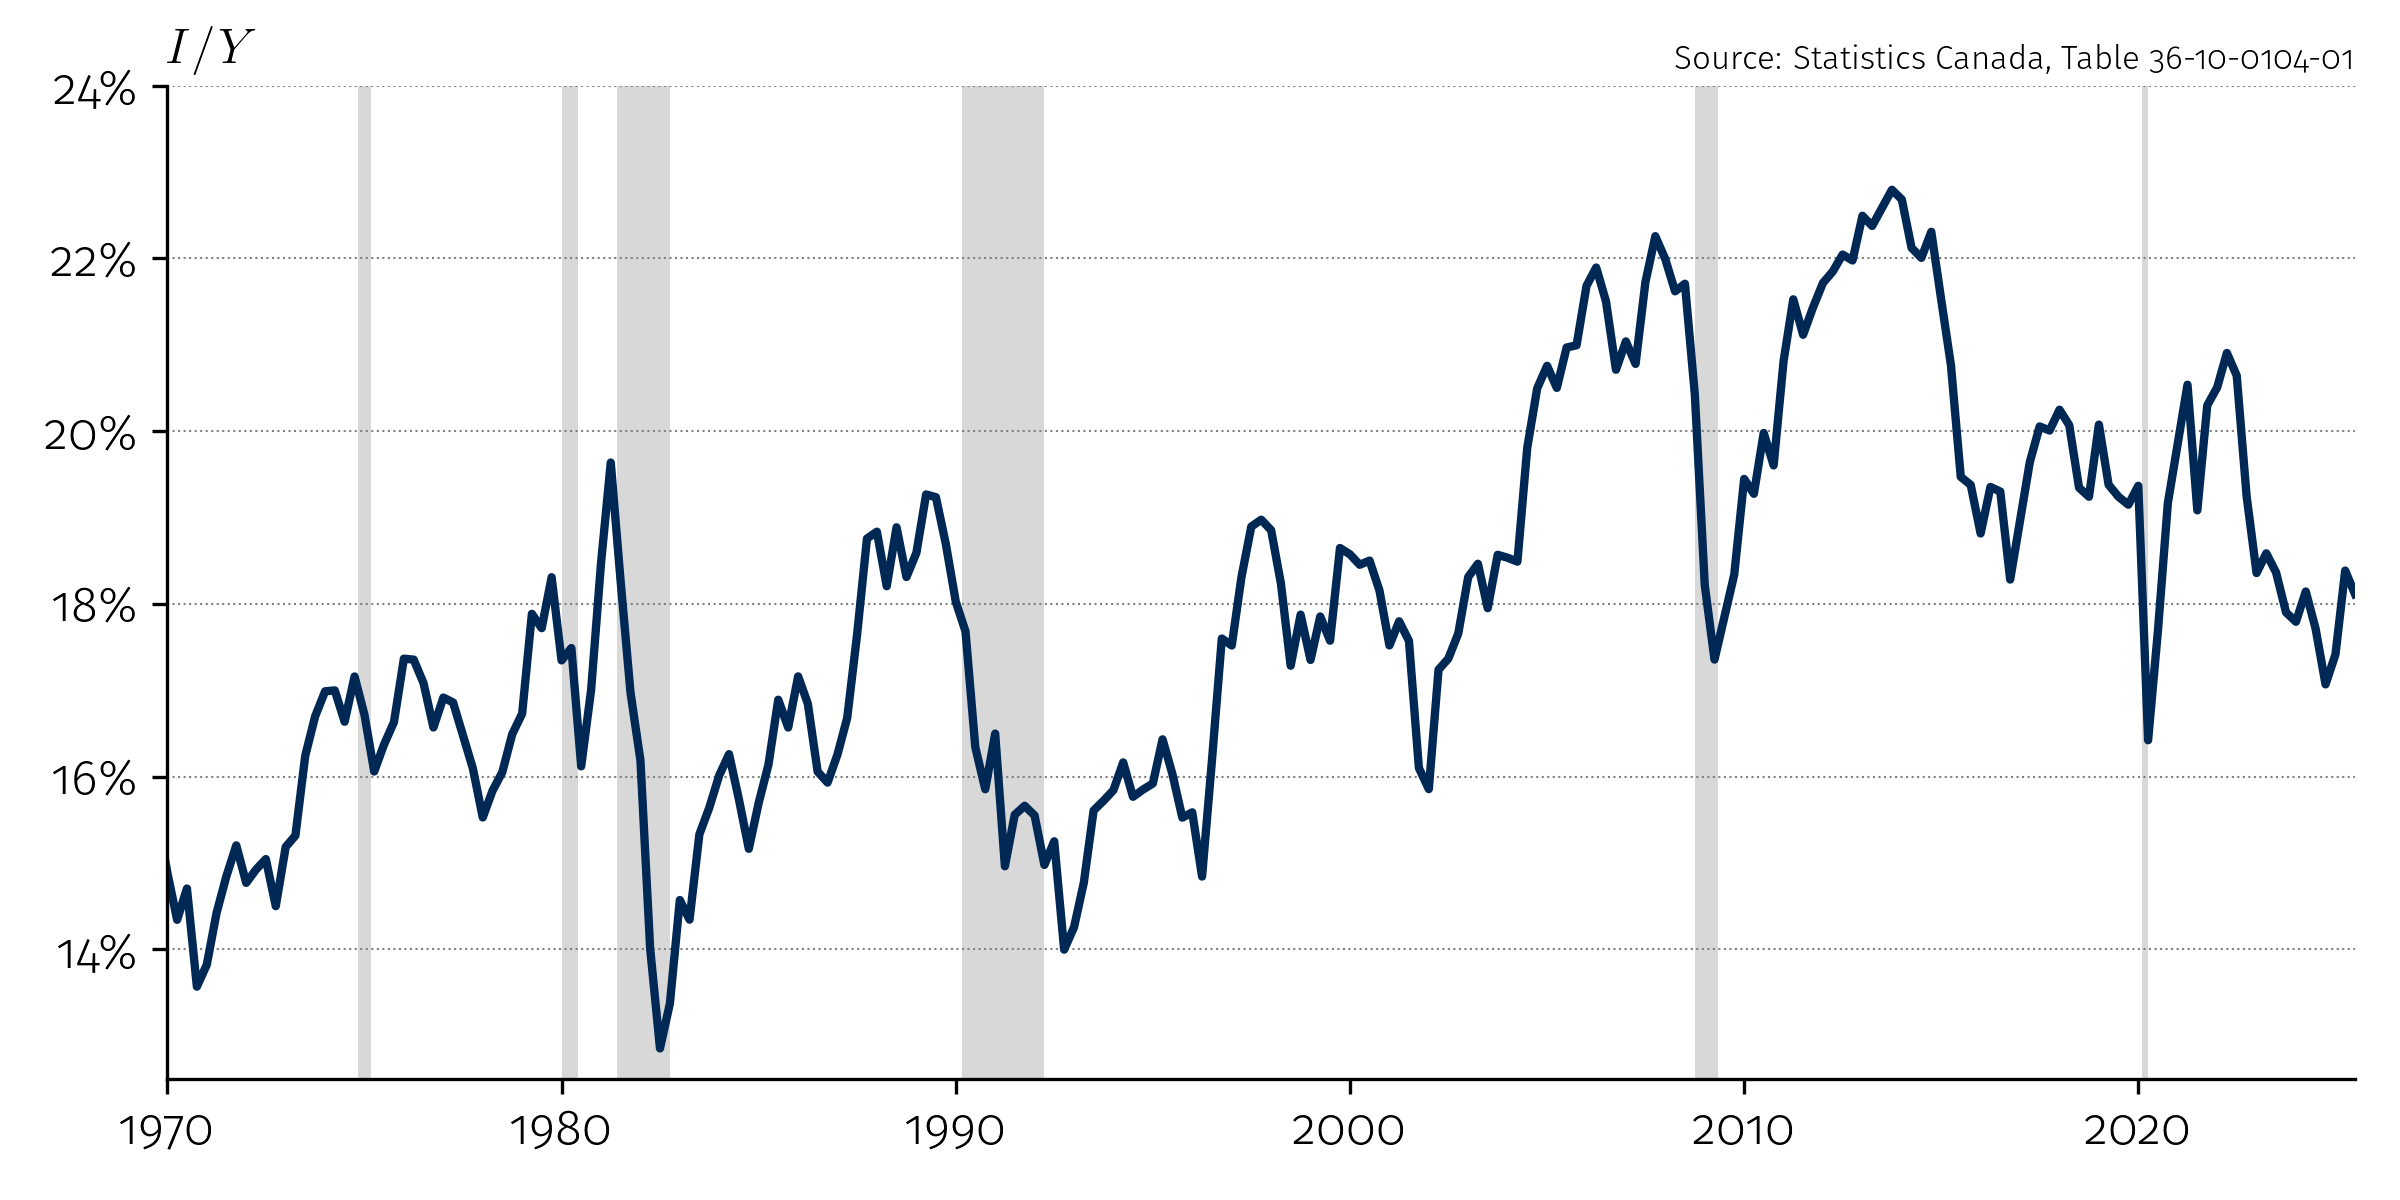
\includegraphics[width=0.95\textwidth]{investment_share_gdp.png}
   \end{figure}
   \vspace{-0.4cm}
   \footnotesize Investment is the most \textbf{volatile} component --- it swings sharply during recessions.
\end{frame}

% ── Government spending ───────────────────────────────────────────────

\begin{frame}[t]{Government spending ($G$)}
   \small
   \textbf{Major producer} of goods/services:
   military, education, healthcare, infrastructure.
   \vspace{0.15cm}
   \begin{defbox}[Valued at cost]
      Often missing market prices, so $G$ measured using \textbf{cost of inputs}.
   \end{defbox}
   \vspace{0.1cm}
   \begin{warning}[Transfers $\neq$ government spending]
      Social transfers (UI, pensions, welfare) are \textbf{not} in $G$ because they do not involve any new production --- they redistribute existing income.
   \end{warning}
\end{frame}

\begin{frame}{Government spending share of GDP in Canada}
   \vspace{-0.2cm}
   \begin{figure}
      \centering
      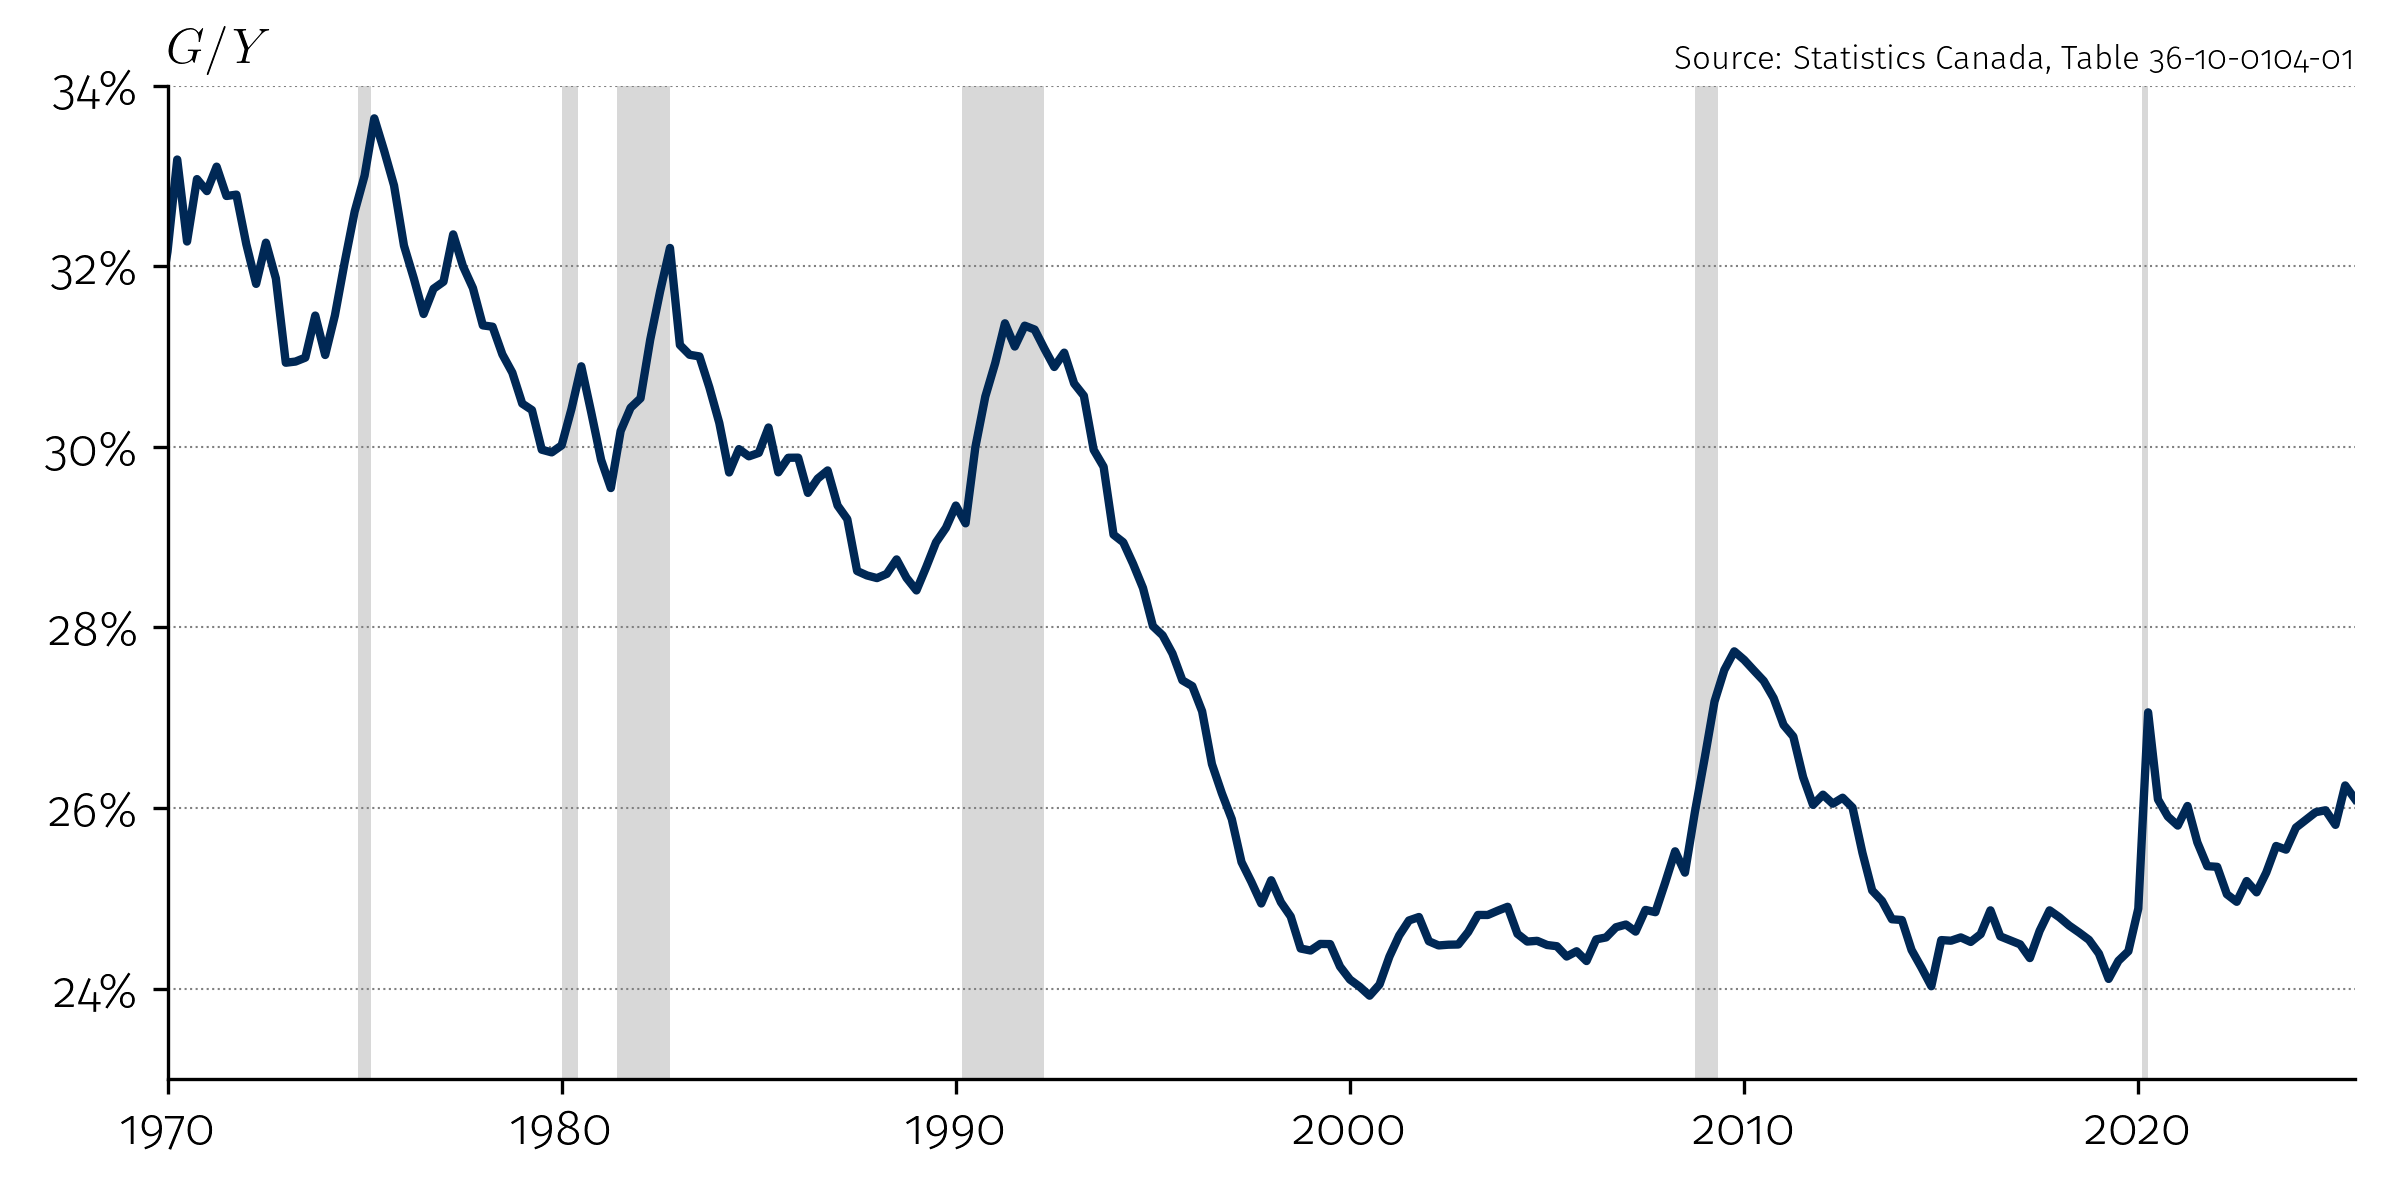
\includegraphics[width=0.95\textwidth]{government_share_gdp.png}
   \end{figure}
   \vspace{-0.4cm}
   \footnotesize Government spending spikes in recessions, but on a long downward trend since the 1990s.
\end{frame}

% ── Exports and imports ───────────────────────────────────────────────

\begin{frame}[t]{Exports and imports ($NX$)}
   $C$, $I$, and $G$ include spending on \textbf{foreign} goods (imports).\\[4pt]
   Since GDP measures \textit{domestic} production, we need a correction:
   \vspace{0.1cm}
   \begin{equation*}
      Y = \underbrace{C + I + G}_{\text{total spending}} + \underbrace{X - M}_{\text{net exports}}
   \end{equation*}
   \vspace{-0.3cm}
   \begin{itemize}
      \setlength\itemsep{0.1cm}
      \item $X$ (exports): domestic production sold to foreigners
      \item $M$ (imports): foreign production already counted in $C$, $I$, $G$
   \end{itemize}
   \vspace{0.15cm}
   \begin{defbox}[Trade openness]
      $(X + M) / Y$ measures how important trade is for an economy.
   \end{defbox}
\end{frame}

\begin{frame}{Trade share of GDP in Canada}
   \vspace{-0.2cm}
   \begin{figure}
      \centering
      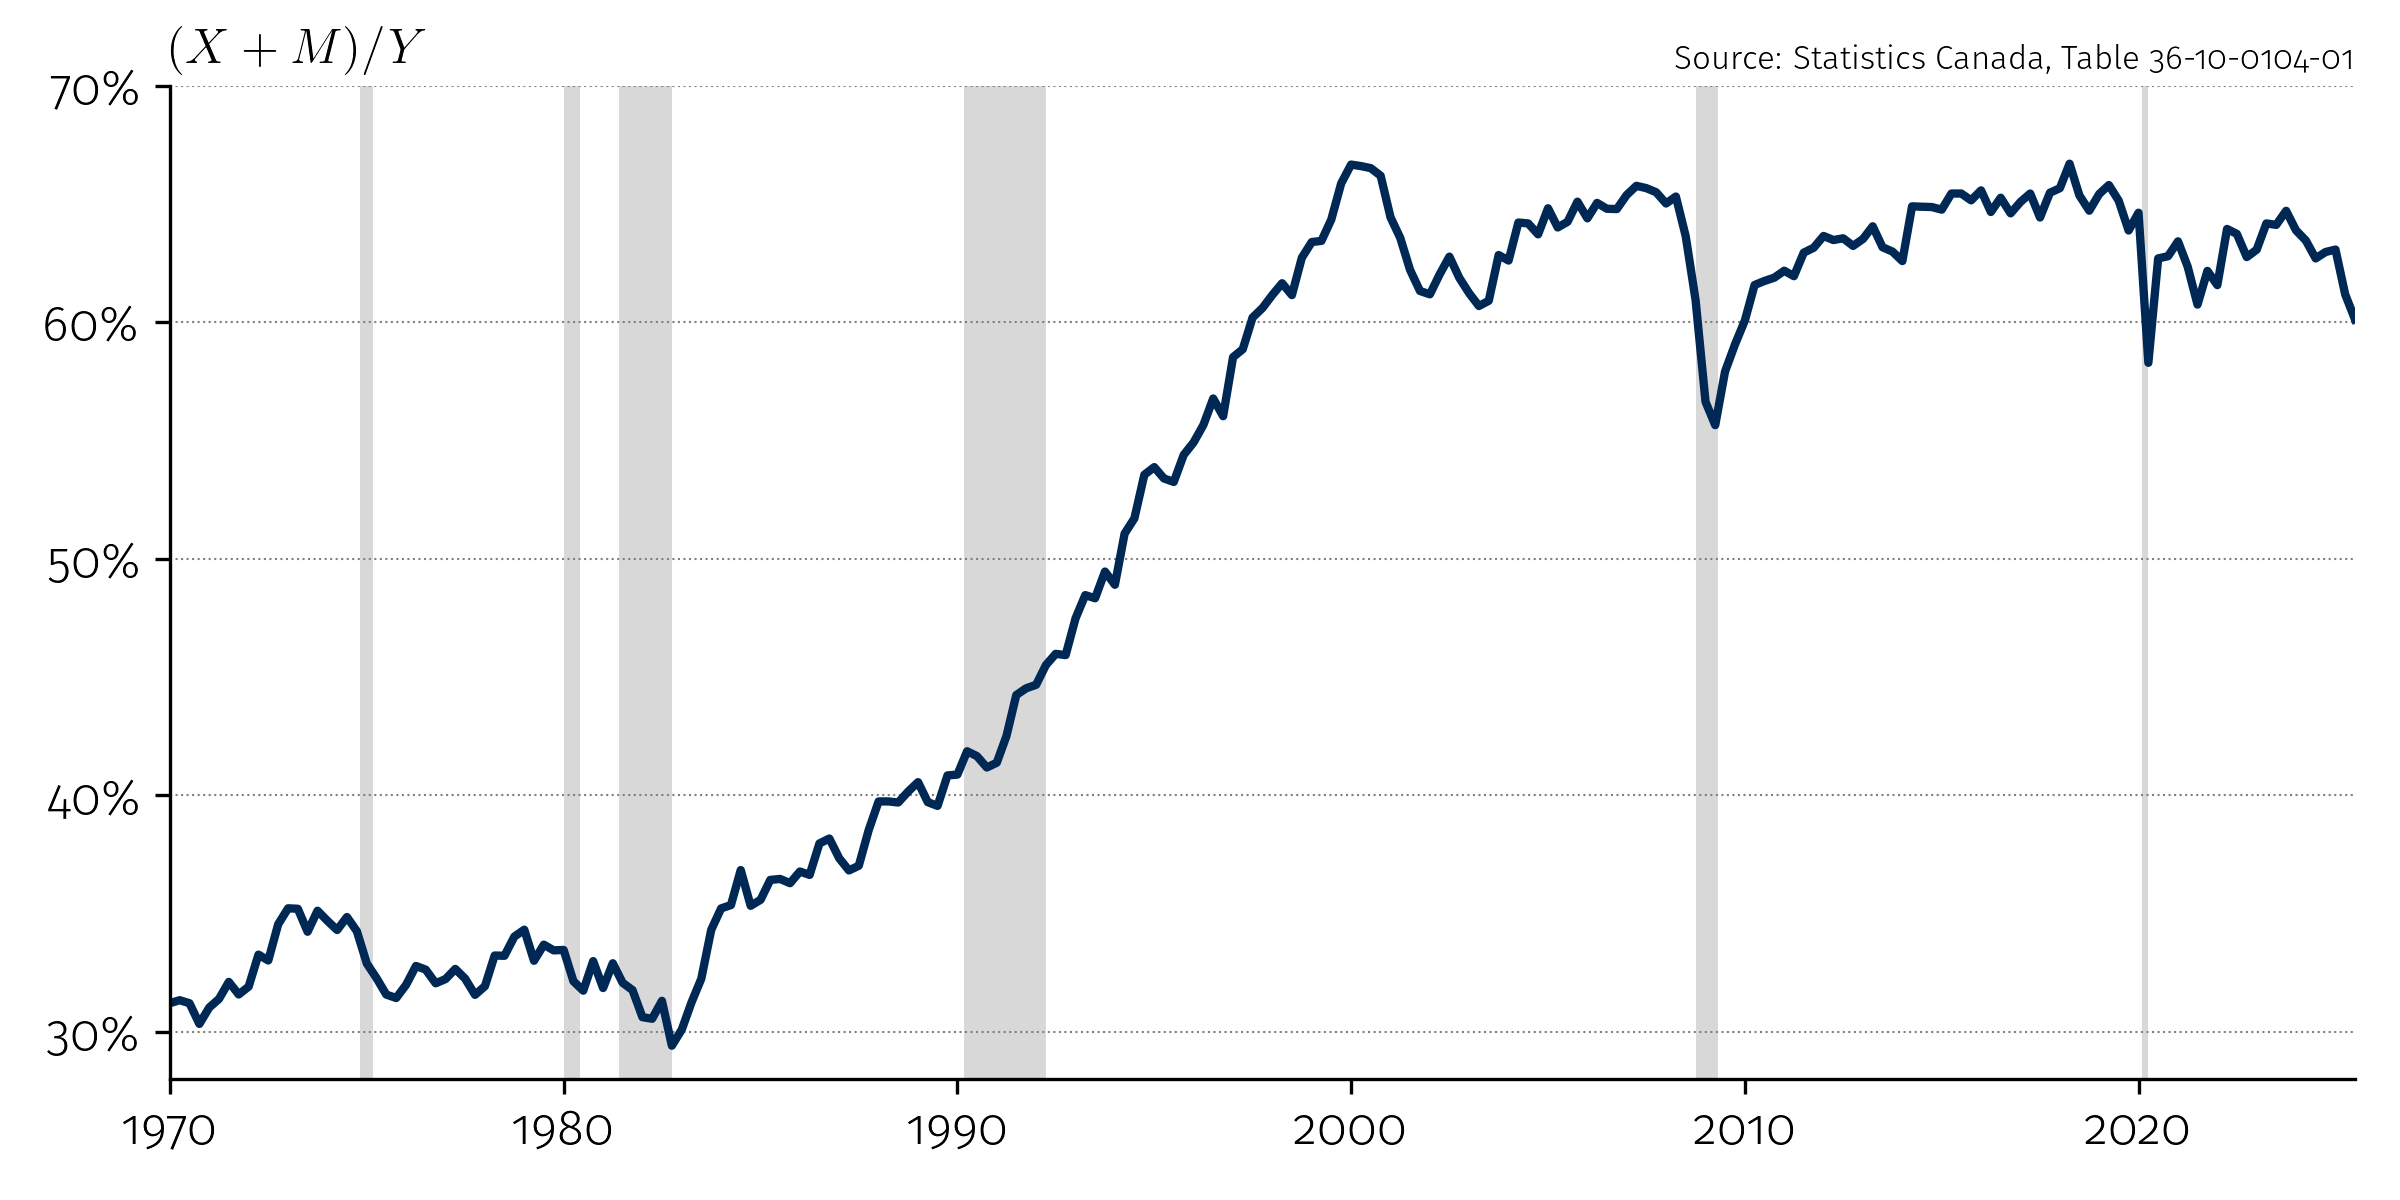
\includegraphics[width=0.95\textwidth]{trade_share_gdp.png}
   \end{figure}
   \vspace{-0.4cm}
   \footnotesize Canada is a very open economy. Trade peaked with NAFTA (1994) and has slightly declined since.
\end{frame}

\begin{frame}[t]{Training your ``BS'' detector}
   \footnotesize
   \vspace{0.1cm}
   \begin{columns}[T]
      \begin{column}{0.42\textwidth}
         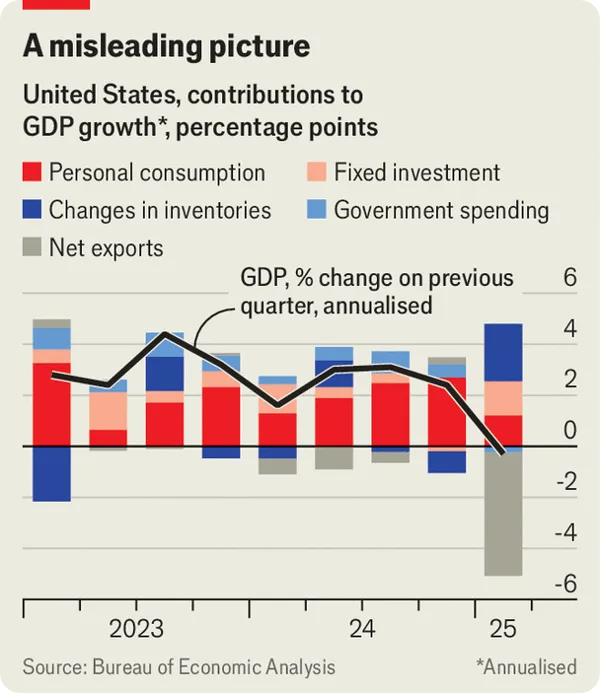
\includegraphics[width=\linewidth, height=0.65\textheight, keepaspectratio]{misleading_GDP_accounting.png}\\[-2pt]
         {\scriptsize\textcolor{HECgray}{Source: \textit{The Economist}, 2025}}
      \end{column}
      \hspace{-2cm}
      \begin{column}{0.54\textwidth}
         In Q1 2025, US GDP fell. Many blamed imports: ``the trade deficit subtracted 5~pp from GDP growth.''
         \vspace{0.15cm}
         \begin{warning}[That's misleading]
            \footnotesize
            Imports enter GDP \textbf{twice}: once \textit{added} in $C$, $I$, or $G$, and once \textit{subtracted} in $NX$.\\[8pt]
            If firms front-load imports before tariffs, inventories surge ($\uparrow I$) while net exports plunge ($\downarrow NX$). The two cancel out.\\[8pt]
            If consumers hurry to buy dishwashers before tariffs, consumption surges ($\uparrow C$) while net exports plunge ($\downarrow NX$). The two cancel out.
         \end{warning}
      \end{column}
   \end{columns}
\end{frame}

\begin{frame}{GDP by expenditure: cross-country comparison}
   \begin{figure}
      \centering
      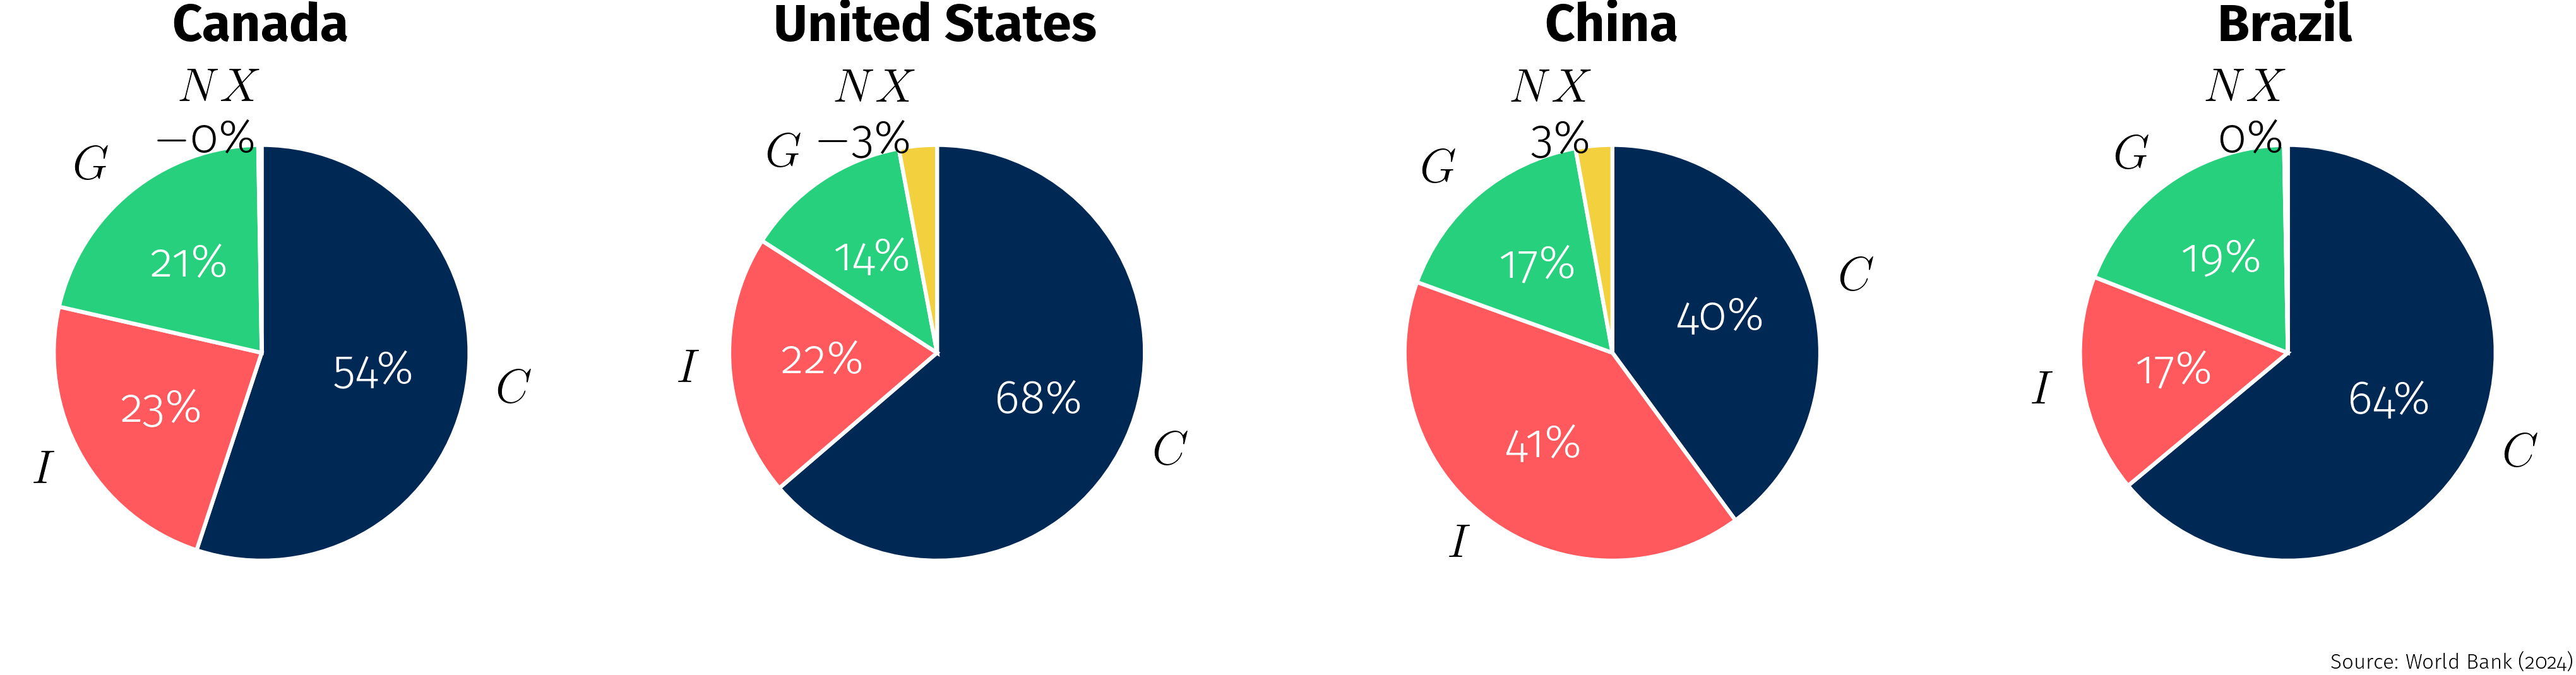
\includegraphics[width=\textwidth]{gdp_decomposition_4countries.png}
   \end{figure}
   \vspace{-0.2cm}
   \begin{keyinsight}[Different growth models]
      China is investment-driven ($I$ = 41\%), while the US is consumption-driven ($C$ = 68\%). These differences shape trade patterns and growth strategies.
   \end{keyinsight}
\end{frame}

\begin{frame}[t]{What GDP does \textit{not} measure}
   GDP only counts \textbf{market transactions}. A lot of economic activity is missed:
   \vspace{0.2cm}
   \begin{itemize}
      \setlength\itemsep{0.15cm}
      \item \textbf{Household production} --- cooking, childcare, home repairs
      \item \textbf{Volunteer work} --- community services, charities
      \item \textbf{Underground economy} --- unreported income, informal work
   \end{itemize}
   \vspace{0.2cm}
   \begin{keyinsight}[Sex, drugs, and GDP]
      In 2014, EU accounting rules began requiring countries to include estimates of illegal activities (e.g., drugs, prostitution) in GDP. Italy's GDP rose by 18\% overnight\ldots
      \hfill{\scriptsize\textit{\color{black!50}The Economist, 2014}}
   \end{keyinsight}
\end{frame}

\begin{frame}{Can we trust GDP figures?}
   \centering
   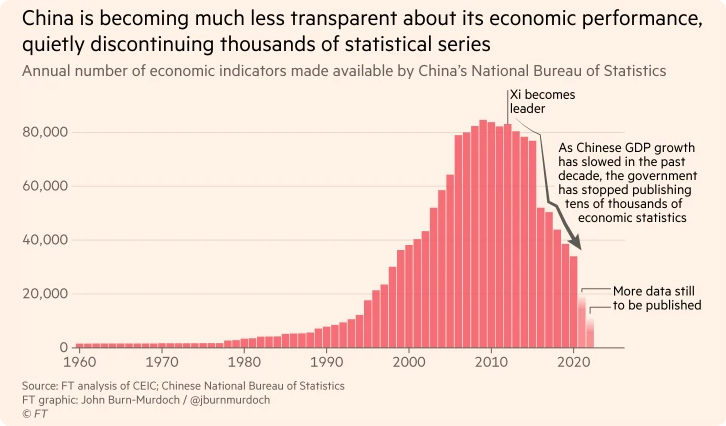
\includegraphics[width=0.75\linewidth, height=0.8\textheight, keepaspectratio]{china_transparency.png}
\end{frame}

\begin{frame}{When data is unavailable\ldots}
   \centering
   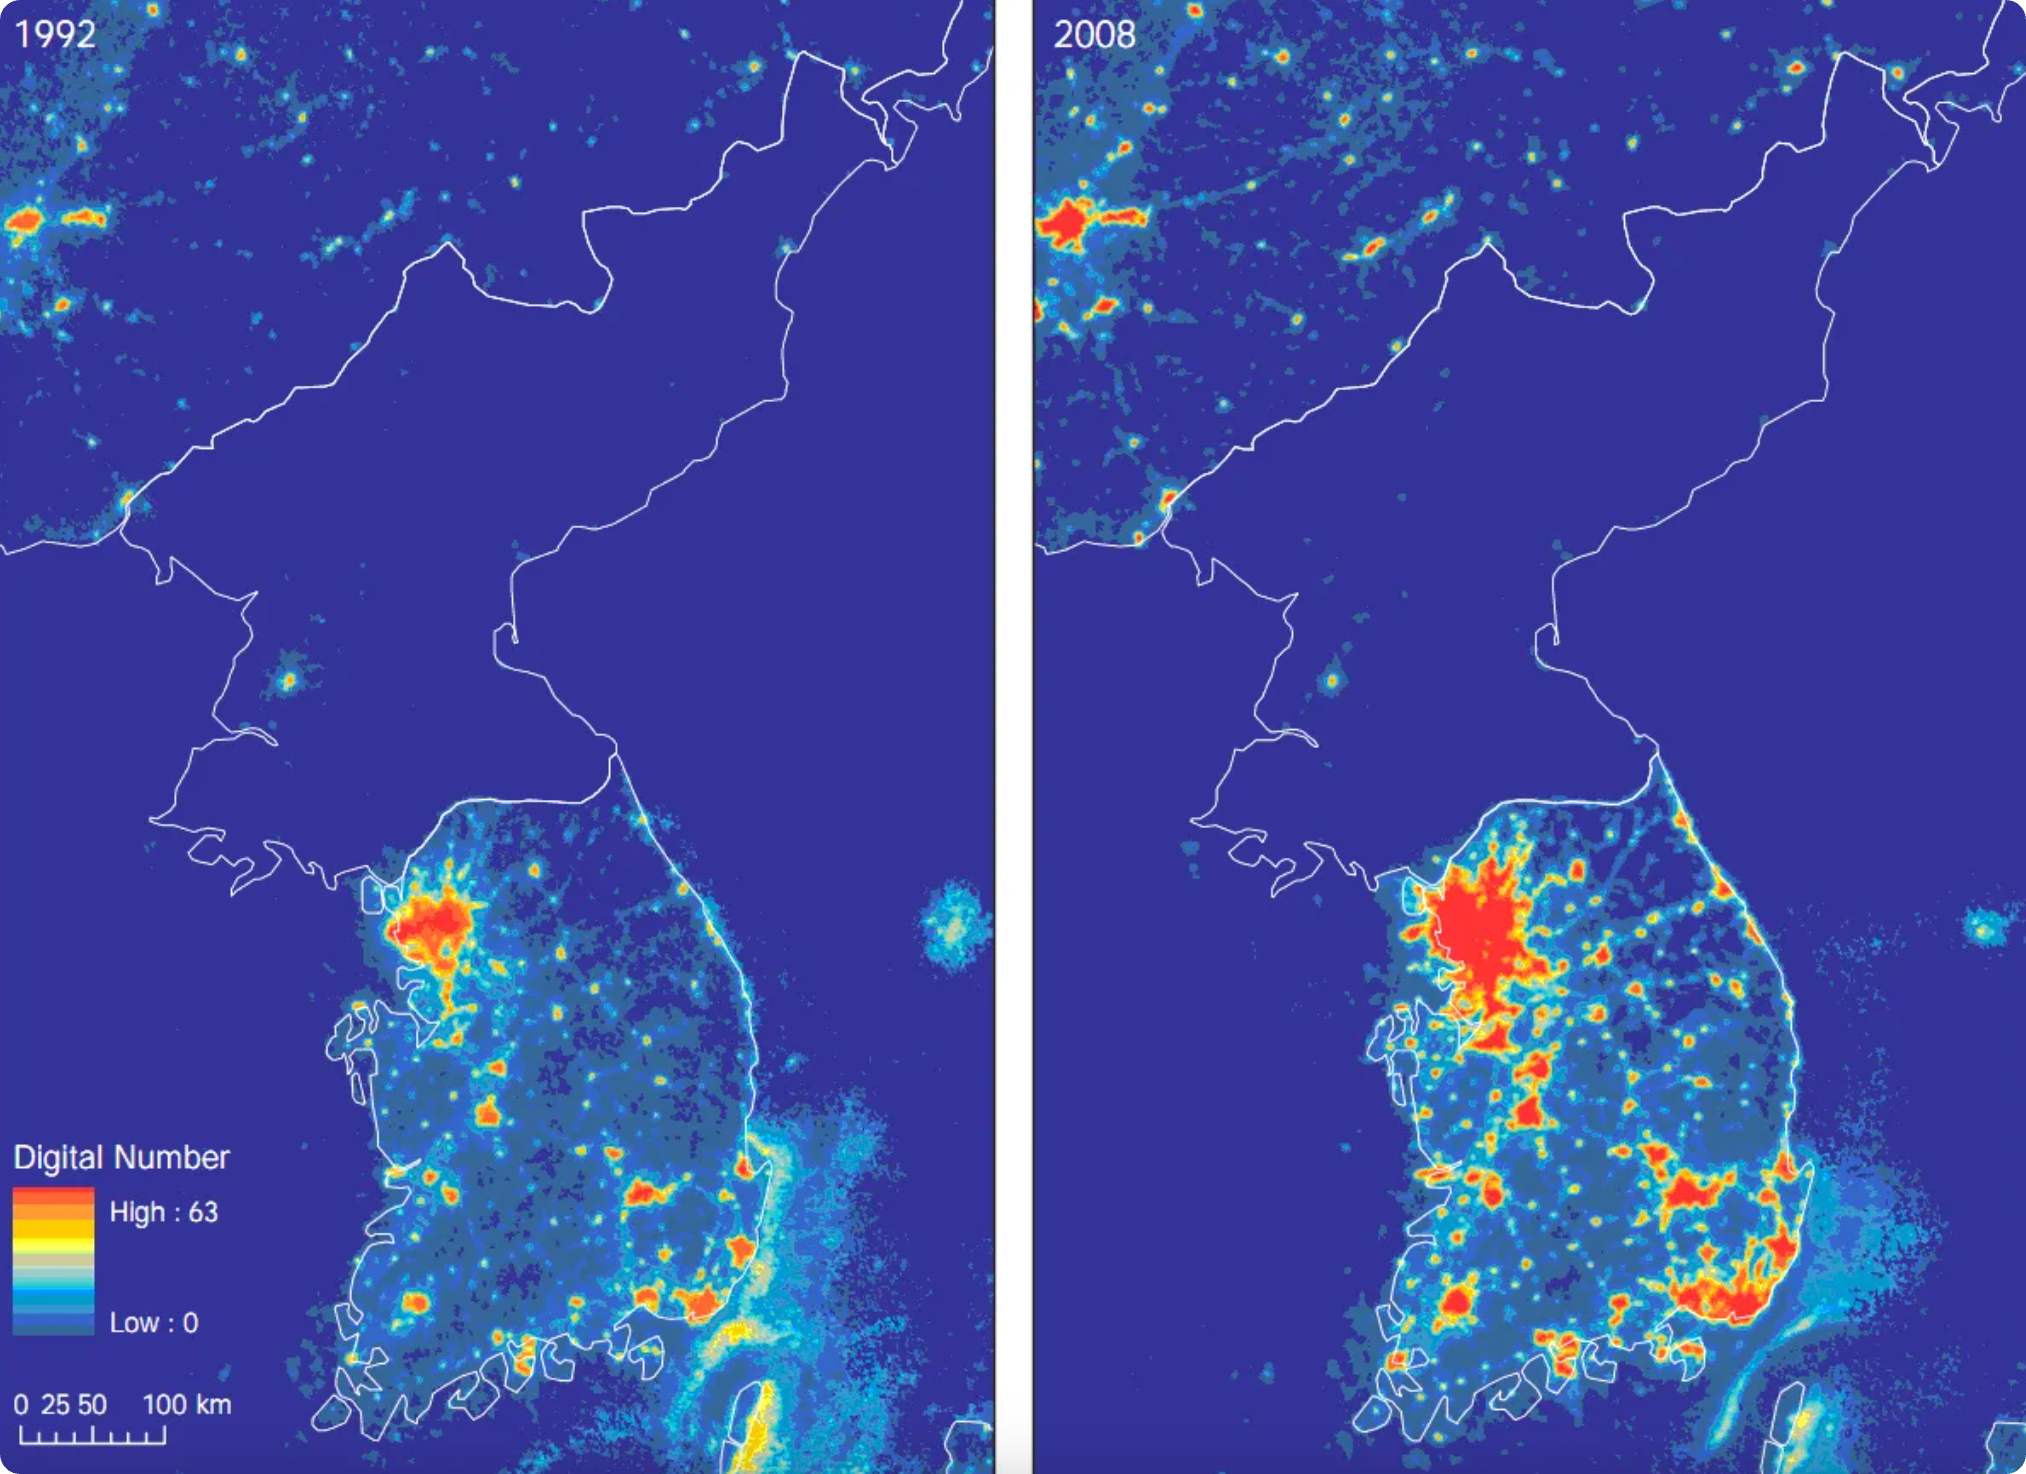
\includegraphics[width=0.75\linewidth, height=0.8\textheight, keepaspectratio]{korea_space.png}
\end{frame}

% ============================================================================
\begin{frame}{Outline}
   \begin{enumerate}
      \setlength\itemsep{0.35cm}
      \item {\color{gray!50}Course overview and logistics}
      \item {\color{gray!50}Measuring the economy: GDP}
      \item \textbf{Measuring inflation}
      \item Comparing living standards across countries
      \item Beyond GDP
      \item The macroeconomic landscape in 2026
   \end{enumerate}
\end{frame}

% ============================================================================
\sectionframe{Measuring inflation}
% ============================================================================

\begin{frame}[t]{Real vs. nominal GDP}
   \begin{defbox}
      \textbf{Nominal GDP} = output at \textit{current} prices. \quad
      \textbf{Real GDP} = output at \textit{constant} prices.
   \end{defbox}
   \vspace{0.05cm}

   \textbf{Example:} nominal GDP grew 5\%, prices rose 3\% $\Rightarrow$ real GDP grew $\sim$2\%.
   \vspace{0.05cm}

   The \textbf{GDP deflator} captures the overall price level:
   \vspace{-0.2cm}
   \begin{equation*}
      \text{GDP deflator} = \frac{\text{Nominal GDP}}{\text{Real GDP}} \times 100
   \end{equation*}
   \vspace{-0.4cm}
   \begin{keyinsight}
      Always use \textbf{real} GDP when comparing output over time. Nominal GDP confounds price and quantity changes.
   \end{keyinsight}
\end{frame}

\begin{frame}{Canadian real GDP since 1960}
   % TODO: Insert FRED or StatCan chart of Canadian real GDP (quarterly, log scale).
   % Show the 1981-82, 1990-91, 2008-09, and 2020 recessions clearly.
   % Source: Statistics Canada, Table 36-10-0104-01
   \begin{figure}
      \centering
      % \includegraphics[width=\textwidth]{real_gdp_canada.png}
      \begin{tcolorbox}[
         colback=HEClightgray, colframe=HECgray, boxrule=0.5pt,
         arc=8pt, width=0.9\textwidth, height=6cm, valign=center
      ]
         \centering
         \textcolor{HECgray}{\small [Figure: Canadian real GDP, 1960--2025, log scale]}\\
         \textcolor{HECgray}{\small Shade the recessions: 1981, 1990, 2008, 2020}
      \end{tcolorbox}
   \end{figure}
\end{frame}

\begin{frame}[t]{Canada's declining standard of living}
   \small
   \begin{columns}[T]
      \begin{column}{0.50\textwidth}
         GDP growth can mask very different \textbf{per capita} dynamics.
         \vspace{0.15cm}
         \begin{itemize}
            \setlength\itemsep{0.1cm}
            \item Canada's real GDP per capita has \textbf{declined} relative to the U.S.\ since 2016
            \item Rapid population growth (immigration) boosted total GDP but \textbf{not per capita}
            \item The U.S.--Canada gap is now at its widest in decades
         \end{itemize}
         \vspace{0.1cm}
         \begin{warning}
            Always look at GDP \textbf{per capita} when assessing living standards. Total GDP can be misleading.
         \end{warning}
      \end{column}
      \begin{column}{0.47\textwidth}
         % TODO: Insert NBF chart: "Canada: Standard of living is declining"
         % Real GDP per capita: Canada vs. the U.S., indexed to 2016Q1=100
         % Source: NBF Economics and Strategy (Statistics Canada and BEA)
         \begin{tcolorbox}[
            colback=HEClightgray, colframe=HECgray, boxrule=0.5pt,
            arc=8pt, height=4.5cm, valign=center
         ]
            \centering
            \textcolor{HECgray}{\small [Figure: Real GDP per capita]}\\
            \textcolor{HECgray}{\small Canada vs.\ U.S., 2016--2024]}\\
            \textcolor{HECgray}{\small Source: NBF / StatCan / BEA}
         \end{tcolorbox}
      \end{column}
   \end{columns}
\end{frame}

% ============================================================================
\sectionframe{Measuring inflation}
% ============================================================================

\begin{frame}{What is inflation?}
   \begin{defbox}[Inflation]
      The rate of change in the \textbf{overall price level} between two periods.
   \end{defbox}
   \vspace{0.3cm}

   \begin{equation*}
      \pi_t = \frac{P_t - P_{t-1}}{P_{t-1}} = \%\Delta P
   \end{equation*}

   where $P_t$ is the price level at time $t$.
   \vspace{0.3cm}

   \textbf{Key question:} how do we measure $P$?
   \vspace{0.2cm}
   \begin{itemize}
      \setlength\itemsep{0.15cm}
      \item \textbf{GDP deflator:} prices of all goods produced domestically (broad)
      \item \textbf{Consumer Price Index (CPI):} prices of a basket of goods bought by consumers (most commonly reported)
   \end{itemize}
\end{frame}

\begin{frame}{The consumer price index (CPI)}
   \begin{columns}[T]
      \begin{column}{0.55\textwidth}
         \textbf{How it works:}
         \vspace{0.15cm}
         \begin{itemize}
            \setlength\itemsep{0.15cm}
            \item Statistical agencies (Statistics Canada, BLS) survey thousands of prices monthly
            \item Prices are weighted by a \textbf{fixed basket} reflecting typical consumer spending
            \item Categories: food, housing, transport, clothing, healthcare, recreation, etc.
         \end{itemize}
         \vspace{0.15cm}
         \textbf{Headline vs. core inflation:}
         \vspace{0.1cm}
         \begin{itemize}
            \footnotesize
            \setlength\itemsep{0.1cm}
            \item \textbf{Headline:} all items (volatile)
            \item \textbf{Core:} excludes food \& energy (less noisy)
         \end{itemize}
      \end{column}
      \begin{column}{0.42\textwidth}
         % TODO: Insert CPI inflation chart for Canada, 2005-2026
         % Show headline vs core measures, with BoC 2% target band
         % Source: Statistics Canada / Bank of Canada
         \begin{tcolorbox}[
            colback=HEClightgray, colframe=HECgray, boxrule=0.5pt,
            arc=8pt, height=5cm, valign=center
         ]
            \centering
            \textcolor{HECgray}{\small [Figure: Canada CPI inflation]}\\
            \textcolor{HECgray}{\small Headline vs.\ core, 2005--2026]}\\
            \textcolor{HECgray}{\small with BoC 2\% target}
         \end{tcolorbox}
      \end{column}
   \end{columns}
\end{frame}

\begin{frame}[t]{Headline vs.\ core inflation}
   \small
   \begin{columns}[T]
      \begin{column}{0.55\textwidth}
         \textbf{Headline inflation} includes all items --- but some are very volatile (food, energy, gasoline).
         \vspace{0.15cm}

         \textbf{Core (underlying) inflation} strips out extreme price changes to reveal the \textbf{trend}.
         \vspace{0.15cm}
         \begin{itemize}
            \setlength\itemsep{0.1cm}
            \item Bank of Canada uses CPI-trim and CPI-median
            \item U.S.\ Fed focuses on ``core PCE'' (excludes food \& energy)
         \end{itemize}
         \vspace{0.1cm}
         \begin{keyinsight}
            Central banks focus on core inflation for policy decisions --- headline inflation is too noisy.
         \end{keyinsight}
      \end{column}
      \begin{column}{0.42\textwidth}
         % TODO: Insert Bank of Canada chart: core inflation range
         % "L'inflation fondamentale a augmenté depuis la fin de 2024"
         % Shows CPI ex indirect taxes and range of core measures, 2019-2025
         % Source: Bank of Canada
         \begin{tcolorbox}[
            colback=HEClightgray, colframe=HECgray, boxrule=0.5pt,
            arc=8pt, height=5cm, valign=center
         ]
            \centering
            \textcolor{HECgray}{\small [Figure: CPI and core inflation]}\\
            \textcolor{HECgray}{\small range, Canada, 2019--2025]}\\
            \textcolor{HECgray}{\small Source: Bank of Canada}
         \end{tcolorbox}
      \end{column}
   \end{columns}
\end{frame}

\begin{frame}[t]{Inflation: why it matters for business}
   \footnotesize
   \begin{columns}[T]
      \begin{column}{0.55\textwidth}
         \textbf{\small Inflation affects:}
         \vspace{0.1cm}
         \begin{itemize}
            \setlength\itemsep{0.08cm}
            \item \textbf{Purchasing power:} wages may not keep up
            \item \textbf{Interest rates:} central banks raise rates to fight inflation
            \item \textbf{Contracts:} long-term deals eroded by unexpected inflation
            \item \textbf{Asset values:} bonds lose value when inflation rises
         \end{itemize}
         \vspace{0.1cm}
         \begin{bizimplication}
            In 2022--23, firms faced a key decision: pass costs to consumers, or absorb them? In 2025, tariffs brought new price pressures.
         \end{bizimplication}
      \end{column}
      \begin{column}{0.42\textwidth}
         % TODO: Insert chart: PriceStats tariff tracker
         % Domestic vs imported goods price index, Nov 2024--Aug 2025
         % Shows imported prices rising after tariff announcements
         % Source: Cavallo, Llamas & Vazquez (2025), PriceStats / State Street
         % https://www.pricinglab.org/tariff-tracker/
         \begin{tcolorbox}[
            colback=HEClightgray, colframe=HECgray, boxrule=0.5pt,
            arc=8pt, height=3.5cm, valign=center
         ]
            \centering
            \textcolor{HECgray}{\small [Figure: Tariff impact on prices]}\\
            \textcolor{HECgray}{\small Domestic vs.\ imported, 2024--25]}\\
            \textcolor{HECgray}{\small Source: PriceStats / Cavallo et al.}
         \end{tcolorbox}
      \end{column}
   \end{columns}
\end{frame}

% ============================================================================
\sectionframe{Comparing living standards\\across countries}
% ============================================================================

\begin{frame}{GDP per capita: enormous variation}
   % TODO: Insert figure from Our World in Data or Penn World Table
   % GDP per capita (PPP, 2017 international $) for selected countries
   \begin{figure}
      \centering
      % \includegraphics[width=\textwidth]{gdp_per_capita_selected.png}
      \begin{tcolorbox}[
         colback=HEClightgray, colframe=HECgray, boxrule=0.5pt,
         arc=8pt, width=0.9\textwidth, height=6cm, valign=center
      ]
         \centering
         \textcolor{HECgray}{\small [Figure: GDP per capita (PPP) since 1950]}\\
         \textcolor{HECgray}{\small US, Canada, Germany, S. Korea, China, India, Nigeria]}\\
         \textcolor{HECgray}{\small Source: Our World in Data / Penn World Table}
      \end{tcolorbox}
   \end{figure}
\end{frame}

\begin{frame}{Comparing GDPs across countries}
   \framesubtitle{Why exchange rates can be misleading}

   \textbf{Two ways to convert GDP into a common currency:}
   \vspace{0.3cm}
   \begin{enumerate}
      \setlength\itemsep{0.3cm}
      \item \textbf{Market exchange rates}
      \begin{itemize}
         \item Useful for comparing \textit{economic power} (e.g., trade, geopolitics)
         \item Problem: very volatile, and ignores price-level differences
      \end{itemize}
      \item \textbf{Purchasing Power Parity (PPP)}
      \begin{itemize}
         \item Adjusts for differences in the cost of living
         \item Better measure of \textit{living standards}
         \item A dollar buys much more in Lagos than in New York
      \end{itemize}
   \end{enumerate}
\end{frame}

\begin{frame}[t]{China vs. United States: it depends how you measure}
   % TODO: Reproduce the China vs US GDP comparison from MBA S2.
   % Two panels side-by-side:
   %   Left: GDP in USD at market exchange rate (US >> China)
   %   Right: GDP in USD at PPP (China > US since ~2016)
   % Source: World Bank or IMF WEO
   \begin{columns}
      \begin{column}{0.48\textwidth}
         \begin{tcolorbox}[
            colback=HEClightgray, colframe=HECgray, boxrule=0.5pt,
            arc=8pt, height=4cm, valign=center
         ]
            \centering
            \textcolor{HECgray}{\small [GDP at market exchange rate]}\\
            \textcolor{HECgray}{\small US $>$ China}
         \end{tcolorbox}
      \end{column}
      \begin{column}{0.48\textwidth}
         \begin{tcolorbox}[
            colback=HEClightgray, colframe=HECgray, boxrule=0.5pt,
            arc=8pt, height=4cm, valign=center
         ]
            \centering
            \textcolor{HECgray}{\small [GDP at PPP]}\\
            \textcolor{HECgray}{\small China $>$ US since $\sim$2016}
         \end{tcolorbox}
      \end{column}
   \end{columns}
   \vspace{0.15cm}
   \begin{warning}[Which measure to use?]
      It depends on the question. Geopolitical influence $\to$ market rates. Living standards $\to$ PPP.
   \end{warning}
\end{frame}

% ============================================================================
\sectionframe{Beyond GDP}
% ============================================================================

\begin{frame}{What GDP does \textbf{not} capture}
   GDP is a useful but incomplete measure of well-being. It misses:
   \vspace{0.3cm}
   \begin{itemize}
      \setlength\itemsep{0.25cm}
      \item \textbf{Inequality:} a country's GDP can grow while most citizens get poorer
      \item \textbf{Non-market production:} household work, childcare, volunteering
      \item \textbf{Environmental costs:} pollution, resource depletion, climate damage
      \item \textbf{Health and well-being:} life expectancy, mental health, leisure time
      \item \textbf{Quality improvements:} your smartphone is infinitely better than a 2005 phone, but GDP struggles to capture this
   \end{itemize}
\end{frame}

\begin{frame}{Growth has lifted millions out of extreme poverty...}
   % TODO: Insert Our World in Data figure on extreme poverty by world region
   % (same as ECON20852 S3 and MBA S3)
   % Source: ourworldindata.org/extreme-poverty
   \begin{figure}
      \centering
      % 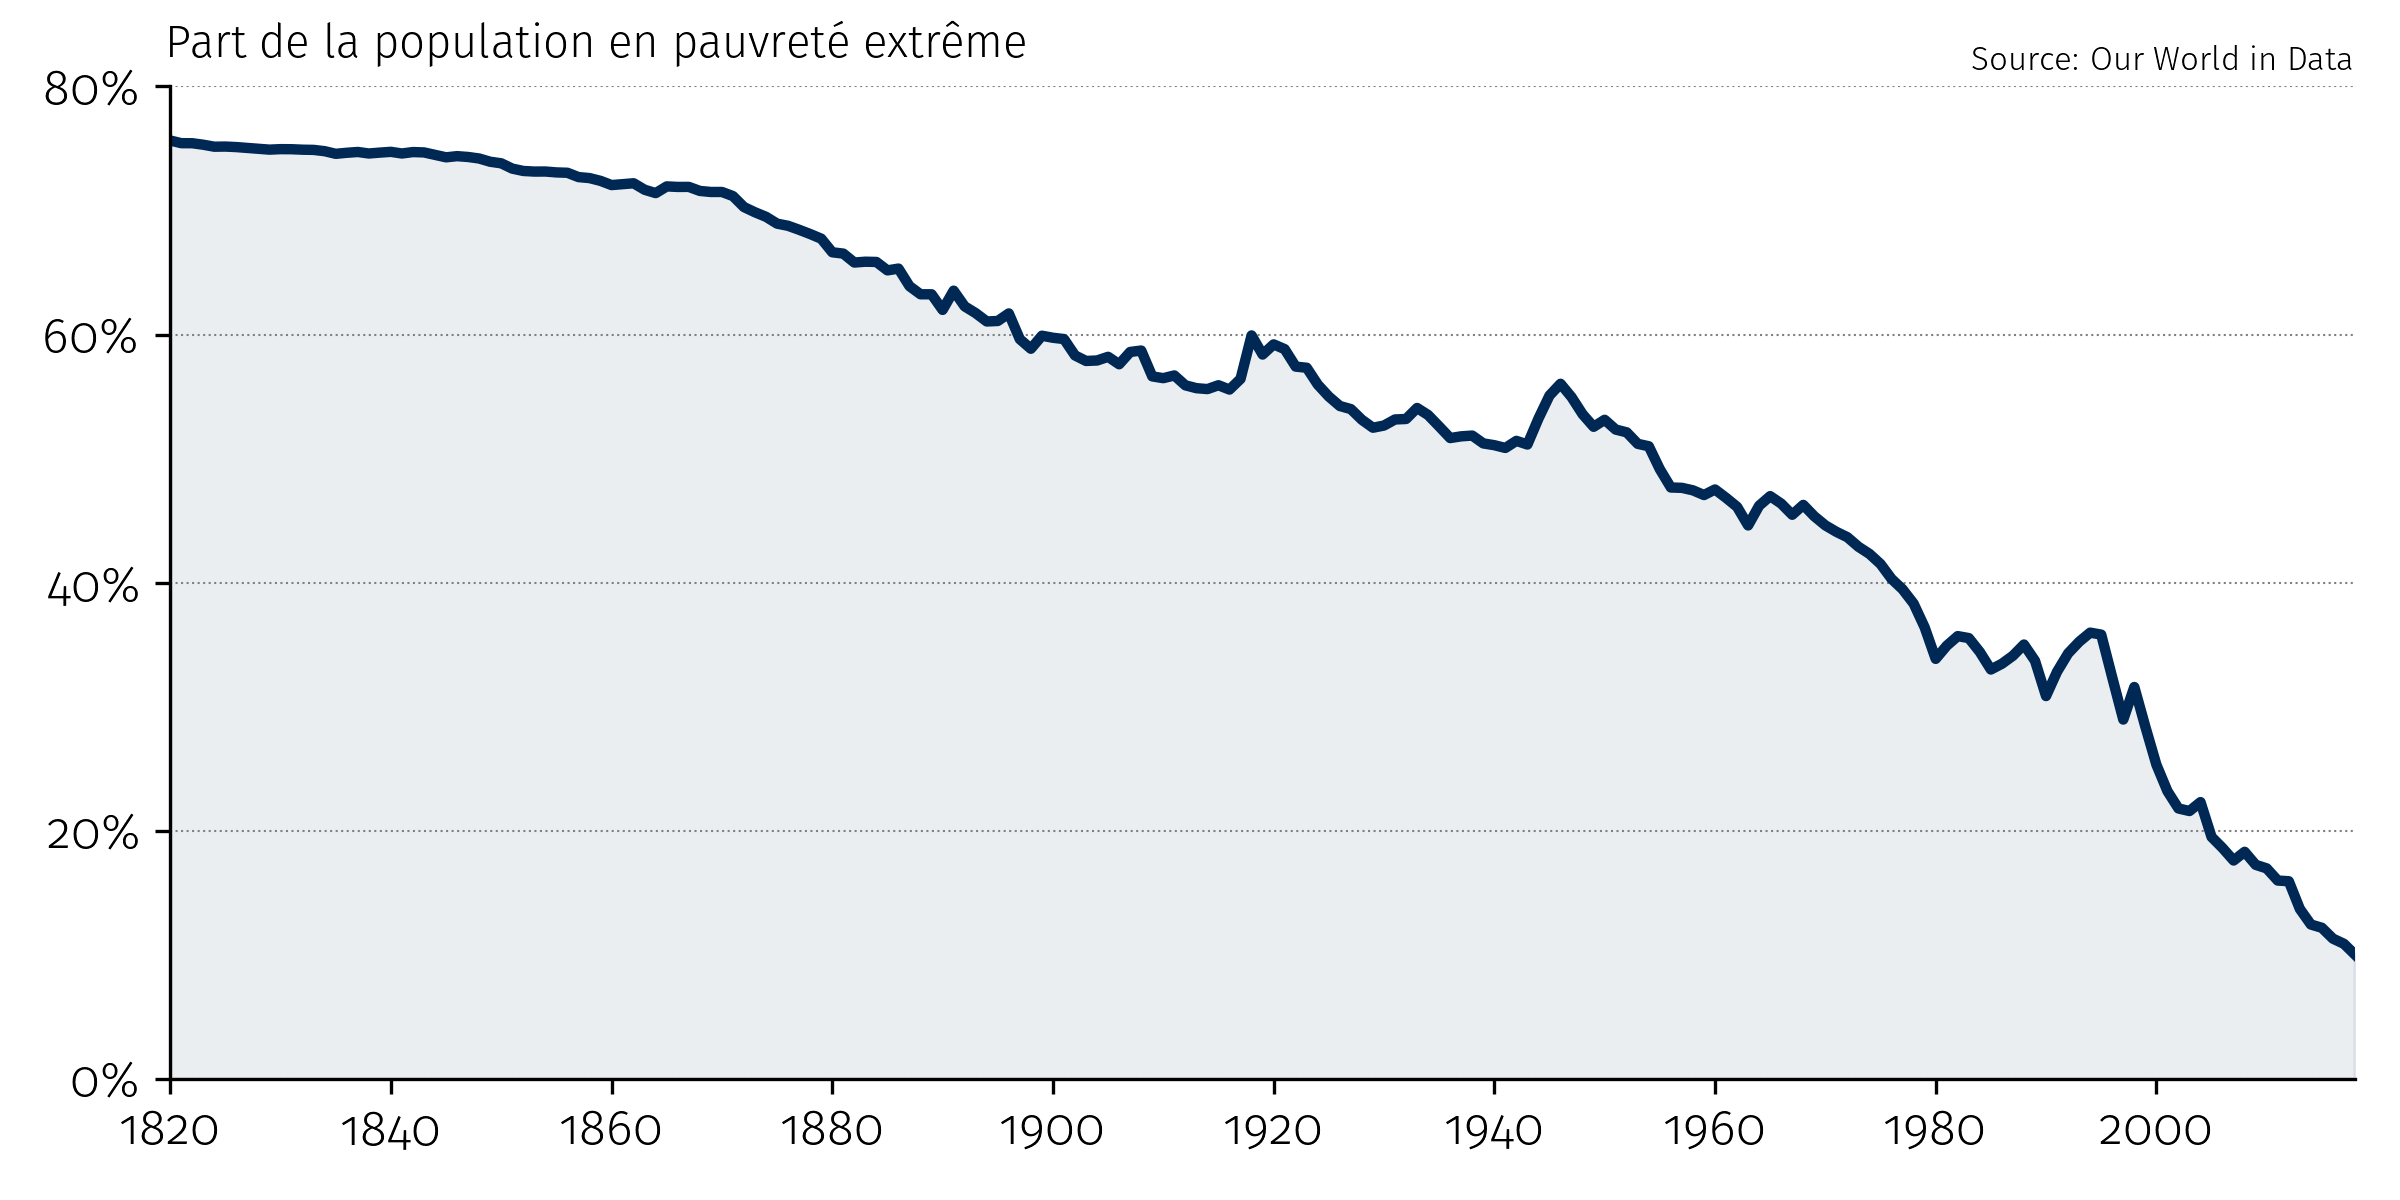
\includegraphics[width=\textwidth]{poverty.png}
      \begin{tcolorbox}[
         colback=HEClightgray, colframe=HECgray, boxrule=0.5pt,
         arc=8pt, width=0.9\textwidth, height=6cm, valign=center
      ]
         \centering
         \textcolor{HECgray}{\small [Figure: Share of population in extreme poverty by region, 1981--2020]}\\
         \textcolor{HECgray}{\small Source: Our World in Data / World Bank}
      \end{tcolorbox}
   \end{figure}
\end{frame}

\begin{frame}{...and saved millions of lives}
   % TODO: Insert Our World in Data figure on life expectancy over time
   % (same as ECON20852 S3 and MBA S3)
   % Source: ourworldindata.org/life-expectancy
   \begin{figure}
      \centering
      % 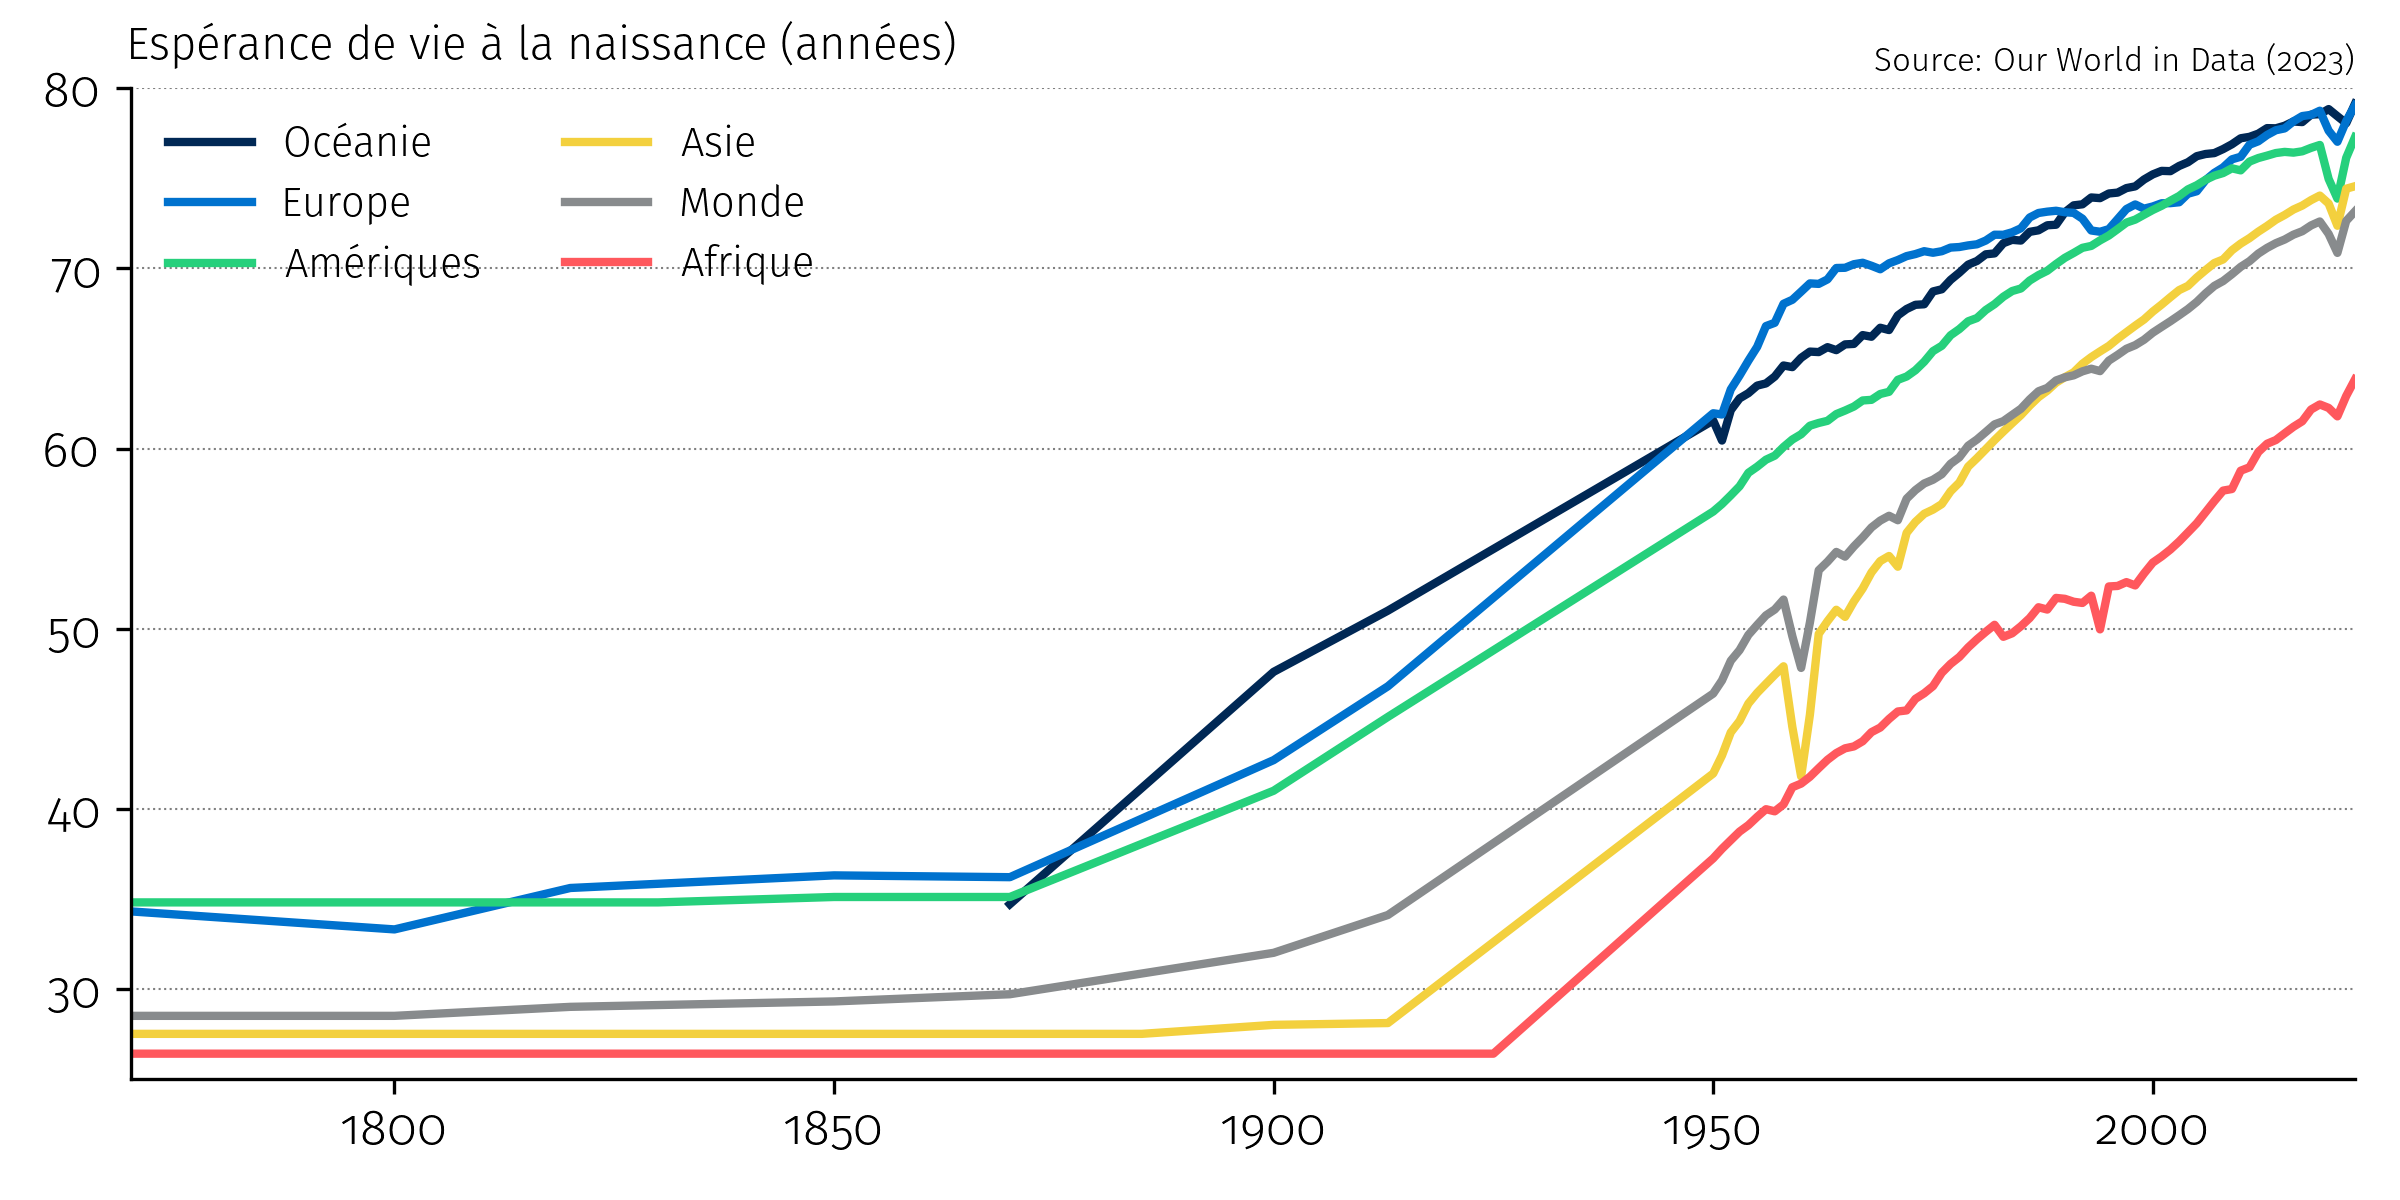
\includegraphics[width=\textwidth]{life_expectancy.png}
      \begin{tcolorbox}[
         colback=HEClightgray, colframe=HECgray, boxrule=0.5pt,
         arc=8pt, width=0.9\textwidth, height=6cm, valign=center
      ]
         \centering
         \textcolor{HECgray}{\small [Figure: Life expectancy at birth, selected countries, 1543--2020]}\\
         \textcolor{HECgray}{\small Source: Our World in Data (Riley, Clio Infra, UN)}
      \end{tcolorbox}
   \end{figure}
\end{frame}

\begin{frame}[t]{But growth alone is not enough}
   \begin{columns}[T]
      \begin{column}{0.55\textwidth}
         \textbf{Growth with rising inequality?}
         \vspace{0.15cm}
         \begin{itemize}
            \setlength\itemsep{0.15cm}
            \item U.S. real GDP per capita has roughly doubled since 1980
            \item But median household income has barely budged
            \item The gains have been concentrated at the top
         \end{itemize}
         \vspace{0.2cm}
         \begin{warning}[For managers]
            Inequality shapes consumer demand, labor markets, regulation, and political risk.
         \end{warning}
      \end{column}
      \begin{column}{0.42\textwidth}
         % TODO: Insert figure showing GDP per capita vs median income in the US
         % Or the "elephant curve" from Lakner-Milanovic
         \begin{tcolorbox}[
            colback=HEClightgray, colframe=HECgray, boxrule=0.5pt,
            arc=8pt, height=5.5cm, valign=center
         ]
            \centering
            \textcolor{HECgray}{\small [Figure: GDP per capita vs.\ median income (US)]}
         \end{tcolorbox}
      \end{column}
   \end{columns}
\end{frame}

% ============================================================================
\sectionframe{The macroeconomic landscape\\in 2026}
% ============================================================================

\begin{frame}{Where we stand today}
   \framesubtitle{Five themes shaping the global economy}

   \small
   \begin{enumerate}
      \setlength\itemsep{0.1cm}
      \item \textbf{Post-pandemic inflation:} supply shocks $\to$ aggressive tightening $\to$ disinflation
      \item \textbf{Interest rate regime shift:} the end of ``free money'' after near-zero rates
      \item \textbf{AI and productivity:} will the AI revolution deliver a sustained productivity boom?
      \item \textbf{Deglobalization:} reshoring, tariffs, and US-China decoupling
      \item \textbf{Canada:} housing affordability, immigration reversal, and fiscal pressures
   \end{enumerate}
   \vspace{0.1cm}
   \begin{bizimplication}
      Each theme connects directly to the analytical tools we will develop in this course.
   \end{bizimplication}
\end{frame}

\begin{frame}[t]{The inflation cycle: a case study in real time}
   % Canadian CPI inflation, 2016-2026 with BoC target band
   % Source: FRED (CPALCY01CAM661N), generated by figures_s1.py
   \vspace{-0.15cm}
   \begin{figure}
      \centering
      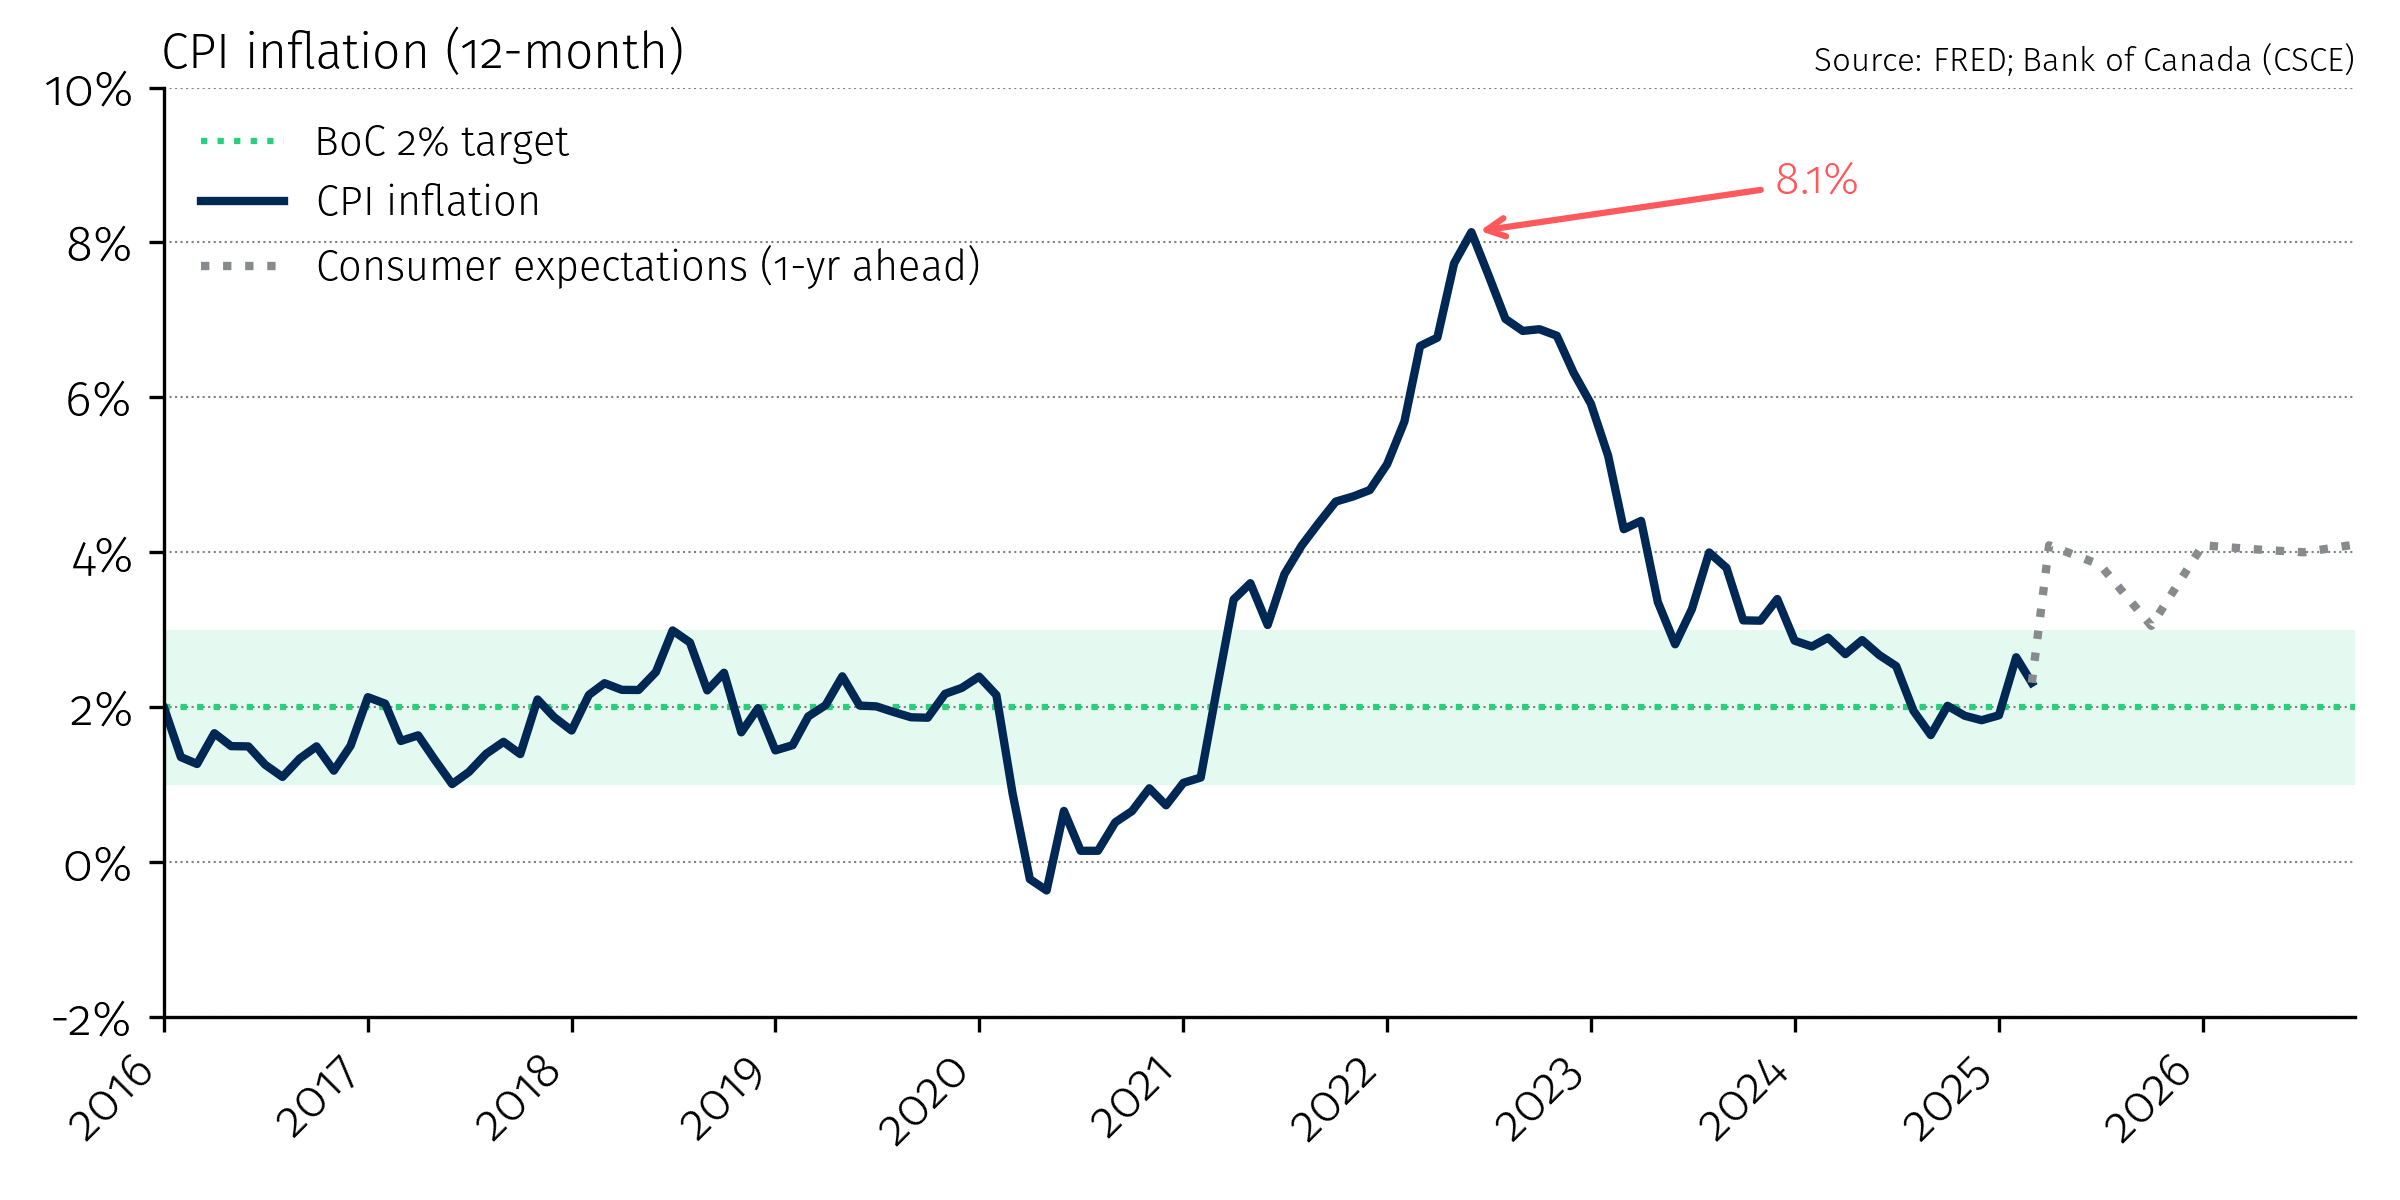
\includegraphics[width=0.85\textwidth, height=4.2cm, keepaspectratio]{canada_inflation_recent.png}
   \end{figure}
   \vspace{-0.25cm}
   \begin{keyinsight}
      In 2021, most economists believed inflation was ``transitory.'' It wasn't. Understanding \textit{why} they were wrong is one of the goals of this course.
   \end{keyinsight}
\end{frame}

\begin{frame}[t]{Interest rates: the end of free money}
   % Policy rates: Fed funds + BoC overnight, 2006-2026
   % Source: FRED (DFF, IRSTCI01CAM156N), generated by figures_s1.py
   \vspace{-0.1cm}
   \begin{figure}
      \centering
      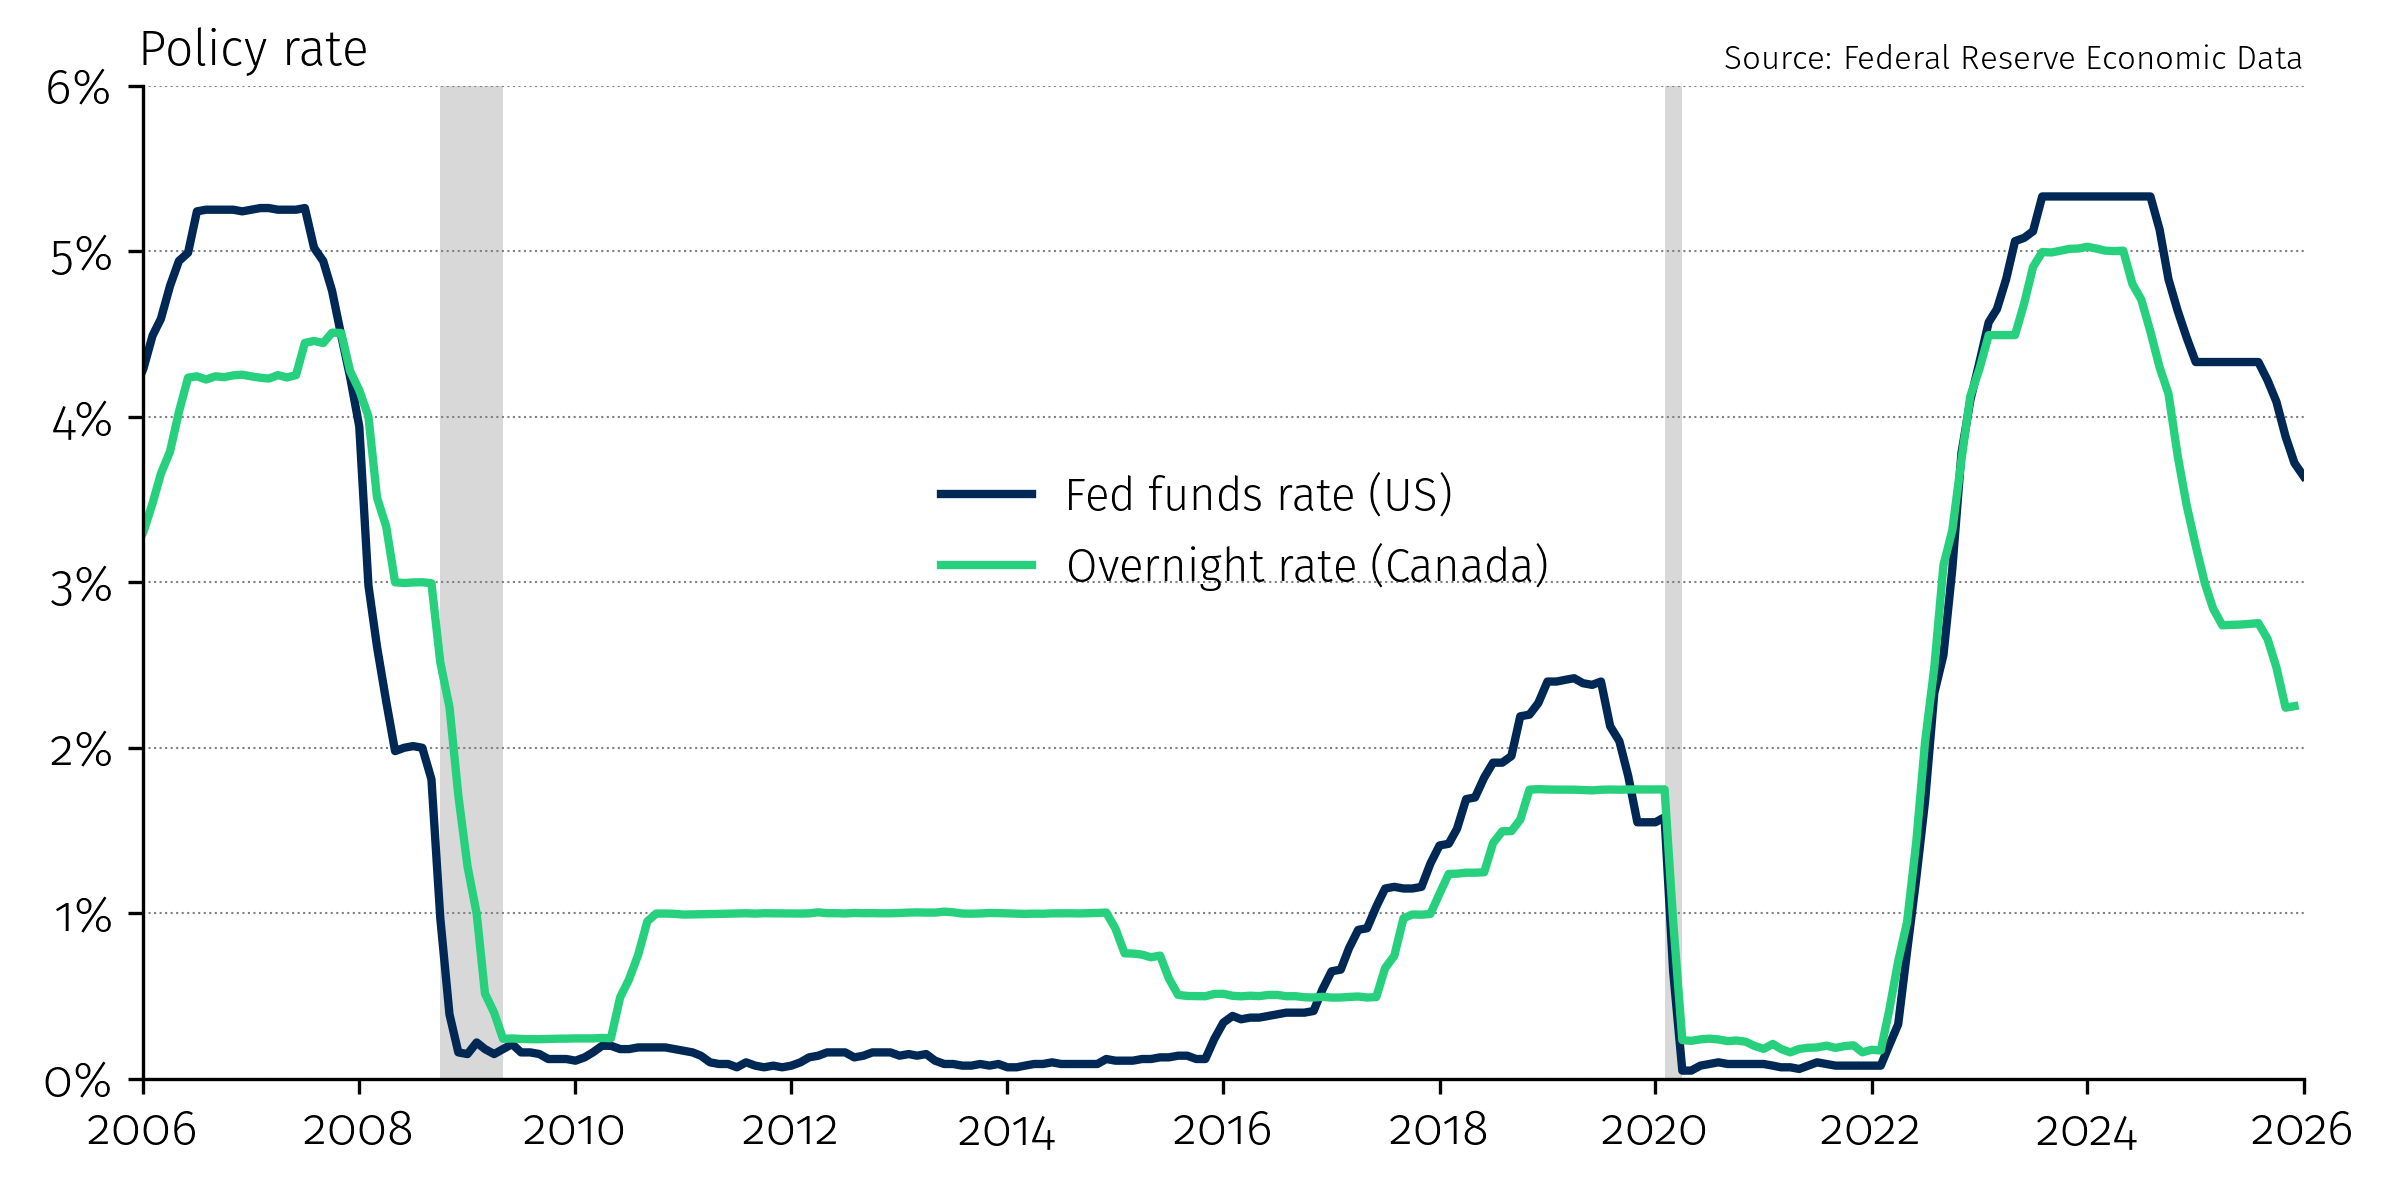
\includegraphics[width=0.85\textwidth, height=4.2cm, keepaspectratio]{policy_rates.png}
   \end{figure}
   \vspace{-0.3cm}
   \begin{bizimplication}
      Higher rates mean higher borrowing costs, lower asset valuations, and a different environment for investment and M\&A.
   \end{bizimplication}
\end{frame}

\begin{frame}[t]{AI and the productivity question}
   \begin{columns}[T]
      \begin{column}{0.55\textwidth}
         \textbf{The big question:}\\[6pt]
         Will AI deliver a new era of productivity growth, or is it mostly hype?
         \vspace{0.3cm}
         \begin{itemize}
            \setlength\itemsep{0.2cm}
            \item \textbf{Optimists:} AI is a general-purpose technology (like electricity)
            \item \textbf{Skeptics:} productivity growth has been disappointing for decades despite previous tech booms
            \item \textbf{The data so far:} massive investment, but productivity gains not yet visible in aggregate statistics
         \end{itemize}
         \vspace{0.2cm}
         {\small We will revisit this in Sessions 2--3.}
      \end{column}
      \begin{column}{0.42\textwidth}
         % TODO: Insert figure on US labor productivity growth (5-year averages)
         % Source: BLS or FRED (OPHNFB)
         \begin{tcolorbox}[
            colback=HEClightgray, colframe=HECgray, boxrule=0.5pt,
            arc=8pt, height=5.5cm, valign=center
         ]
            \centering
            \textcolor{HECgray}{\small [Figure: U.S.\ labor productivity growth]}\\
            \textcolor{HECgray}{\small 5-year averages, 1950--2025}
         \end{tcolorbox}
      \end{column}
   \end{columns}
\end{frame}

\begin{frame}[t]{Deglobalization and trade tensions}
   \small
   \begin{columns}[T]
      \begin{column}{0.55\textwidth}
         \textbf{The world is fragmenting:}
         \vspace{0.15cm}
         \begin{itemize}
            \setlength\itemsep{0.15cm}
            \item US-China decoupling accelerating
            \item U.S.\ effective tariff rate at highest in nearly a century ($\sim$17\%, Smoot-Hawley levels)
            \item ``Reshoring'' and ``friend-shoring'' as strategy
            \item Supply chain resilience vs.\ efficiency
         \end{itemize}
         \vspace{0.1cm}
         \begin{warning}[For business]
            Global supply chains built over decades are being restructured. This creates both risks and opportunities.
         \end{warning}
      \end{column}
      \begin{column}{0.42\textwidth}
         % TODO: Insert chart for this column
         % (tariff rate figure moved to narrative arc slide N5)
         \begin{tcolorbox}[
            colback=HEClightgray, colframe=HECgray, boxrule=0.5pt,
            arc=8pt, height=5cm, valign=center
         ]
            \centering
            \textcolor{HECgray}{\small [Figure: Progression of Trump tariffs]}\\
            \textcolor{HECgray}{\small US effective tariff rate, 2025}\\
            \textcolor{HECgray}{\small Source: FT / Yale Budget Lab}
         \end{tcolorbox}
      \end{column}
   \end{columns}
\end{frame}

\begin{frame}[t]{Canada: the tariff impact in real time}
   \small
   \begin{columns}[T]
      \begin{column}{0.55\textwidth}
         The Canadian economy \textbf{contracted} in Q2 2025, driven by a collapse in exports to the U.S.
         \vspace{0.15cm}
         \begin{itemize}
            \setlength\itemsep{0.1cm}
            \item Employment in export-dependent sectors \textbf{fell sharply} while other sectors grew
            \item $\sim$75\% of Canadian exports go to the U.S.
            \item Bank of Canada cut rates aggressively in response
         \end{itemize}
         \vspace{0.1cm}
         \begin{bizimplication}
            The GDP expenditure identity in action: a drop in $NX$ directly reduces $Y$. We will explore these mechanics throughout the course.
         \end{bizimplication}
      \end{column}
      \begin{column}{0.42\textwidth}
         % TODO: Insert Bank of Canada chart: GDP growth decomposition
         % Contribution to real GDP growth, Q2 2024 -- Q2 2025
         % Shows contraction in 2025Q2 driven by exports
         % Source: Statistics Canada, Bank of Canada estimates
         \begin{tcolorbox}[
            colback=HEClightgray, colframe=HECgray, boxrule=0.5pt,
            arc=8pt, height=5cm, valign=center
         ]
            \centering
            \textcolor{HECgray}{\small [Figure: Canada GDP decomposition]}\\
            \textcolor{HECgray}{\small Q2 2025 contraction]}\\
            \textcolor{HECgray}{\small Source: Bank of Canada}
         \end{tcolorbox}
      \end{column}
   \end{columns}
\end{frame}

\begin{frame}{Canada in the global picture}
   \textbf{Key challenges for the Canadian economy:}
   \vspace{0.1cm}
   \small
   \begin{itemize}
      \setlength\itemsep{0.1cm}
      \item \textbf{Housing affordability:} prices have far outpaced incomes, especially in major cities
      \item \textbf{Immigration policy:} rapid population growth strained housing and services; government reversed course
      \item \textbf{Productivity gap:} Canadian productivity growth has consistently lagged the U.S.
      \item \textbf{Trade exposure:} $\sim$75\% of exports go to the U.S. --- tariff risks are existential
      \item \textbf{Declining living standards:} real GDP per capita has fallen relative to the U.S.
      \item \textbf{Fiscal pressures:} pandemic deficits pushed public debt to new highs
   \end{itemize}
   \vspace{0.1cm}
   \begin{bizimplication}
      Many of these challenges intersect. We will study each through the lens of macro theory.
   \end{bizimplication}
\end{frame}

% ============================================================================
\sectionframe{Where this course is going}
% ============================================================================

\begin{frame}{Connecting the themes to the course}
   \renewcommand{\arraystretch}{1.5}
   \centering
   \small
   \begin{tabular}{>{\bfseries}l l}
      \toprule
      \textbf{Theme} & \textbf{Course sessions} \\
      \midrule
      Why are some countries rich? & S2: Long-run growth \\
      AI, inequality, labor shortages & S3: Labor market \\
      Where does inflation come from? & S4: Money \& business cycles \\
      Rate hikes, stimulus, debt & S5: Monetary \& fiscal policy \\
      Trade, exchange rates, China & S6: Financial markets \& international \\
      \bottomrule
   \end{tabular}
\end{frame}

% ============================================================================
\takeawayframe{Key takeaways}{%
   \small
   \begin{enumerate}
      \setlength\itemsep{0.08cm}
      \item \textbf{GDP} measures the total value of final goods and services produced in a country
      \item The expenditure identity ($Y = C + I + G + NX$) is the backbone of macro accounting
      \item Always use \textbf{real GDP per capita} over time and \textbf{PPP-adjusted GDP} across countries
      \item \textbf{Inflation} (measured by CPI) tracks changes in the cost of living --- focus on \textbf{core} measures for the trend
      \item GDP data is imperfect: think critically about the numbers and who produces them
      \item The 2026 landscape: tariff disruptions, declining Canadian living standards, AI, and the end of ``free money''
   \end{enumerate}
}

% ============================================================================

\begin{frame}{Before next class}
   \textbf{Readings:}
   \vspace{0.15cm}
   \begin{itemize}
      \setlength\itemsep{0.15cm}
      \item Vincent \& Yared, Chapters 1--2
      % TODO: Update with actual assigned readings
   \end{itemize}
   \vspace{0.4cm}
   \textbf{To think about:}
   \vspace{0.15cm}
   \begin{itemize}
      \setlength\itemsep{0.15cm}
      \item Pick a country. Look up its GDP per capita (PPP). What surprised you?
      \item Find a recent macroeconomic headline. What questions does it raise?
   \end{itemize}
\end{frame}

\end{document}
